\documentclass[10pt,a4paper]{article}
\usepackage[utf8]{inputenc}
\usepackage[T1]{fontenc}
\usepackage{amsmath}
\usepackage{amssymb}
\usepackage{bm}
\usepackage{graphicx}
\usepackage{booktabs}
\usepackage{longtable}
\usepackage{array}
\usepackage{hyperref}

% -------- custom macros (kept in sync with main.tex) --------
\newcommand{\dtgsk}{DT-GSK}
\newcommand{\sgsm}{SGSM}
\newcommand{\atmals}{ATMALS-GSK}
\newcommand{\agsk}{AGSK}
\newcommand{\apgsk}{APGSK}
\newcommand{\fdbagsk}{FDB-AGSK}
\newcommand{\egsk}{eGSK}
\newcommand{\bestval}[1]{\textbf{#1}}
\newcommand{\wmark}{\ensuremath{+}}
\newcommand{\lmark}{\ensuremath{-}}
\newcommand{\emark}{\ensuremath{\approx}}
\newcommand{\argmin}{\operatorname{arg\,min}}
\newcommand{\argmax}{\operatorname{arg\,max}}
\newcommand{\tablesize}[1]{}
\newcommand{\reftitle}[1]{}
\newcommand{\externalbibliography}[1]{}

\title{DT-GSK: Dimension-Tiered Adaptive Control and Deterministic Refinement for Gaining-Sharing Knowledge Optimization}
\author{Mostafa Elsayed Masoud @@SUP!1,*@@, Heba Sayed Mohamed Roshdy @@SUP!1@@ and Ali Wagdy Mohamed @@SUP!1@@}
\date{}

\begin{document}
\noindent\textit{Article}

\maketitle

\begin{center}\footnotesize
@@SUP!1@@ \quad Operations Research Department, Faculty of Graduate Studies for
Statistical Research, Cairo University, Giza 12613, Egypt;
% The iDs are written LITERALLY here, not via \orcidauthorA/B: pandoc does not
% expand custom LaTeX macros, so the macro form rendered in the PDF but silently
% vanished from the DOCX (verified 2026-07-25) -- a cross-format inconsistency.
% The macro definitions above are kept because MDPI's template expects them.
moustafa.masoud@gmail.com (M.E.M.\ ORCID 0009-0003-8415-2158); hmhmdss@yahoo.com (H.S.M.R.\ ORCID 0000-0003-0387-5876); aliwagdy@gmail.com (A.W.M.\ ORCID 0000-0002-5895-2632)\\
* Correspondence: moustafa.masoud@gmail.com
\end{center}

\begin{abstract}
Published gaining-sharing knowledge (GSK) variants adapt scalar control and
donor/selection policy at one operating point. Dimension-Tiered
Gaining-Sharing Knowledge (DT-GSK) instead resolves control by
dimension: an adaptive scaffold serves every tier, a deterministic,
budget-exact eigenframe refinement runs once from $D = 50$ upward, and the
GSK vector-update equations are retained; an exploratory
interaction-structure memory, learned from accepted moves at no extra
evaluations, supplies the refinement basis.
Against six GSK-family baselines re-executed in-repository on CEC2017
(primary), CEC2011, CEC2013, CEC2020, and CEC2013LSGO under one
budget-fair paired protocol, DT-GSK attains the best descriptive
family-rank aggregate on CEC2017 (2.48) and CEC2013 (2.80); it is second
behind eGSK at $D = 30$ and on CEC2011; the CEC2011 loss is
Holm-significant. % BIND: AN-RANKAGG-2017-OVERALL (friedman_ranks_cec2017_overall.csv; RS-01 NARROWED); AN-RANKAGG-2013-OVERALL (friedman_ranks_cec2013_overall.csv); AN-OMNI-2011-NATIVE (friedman_ranks_cec2011.csv)
On AGSK's strongest suite---the CEC2020 competition in which it was the
runner-up---DT-GSK places fourth; the family panel corroborates AGSK's
published strength in this regime, consistent with the tiering thesis:
every dimension-gated DT-GSK subsystem is inactive at
$D \leq 20$. % BIND: RS-12 (SAP addendum Sec. 9 [AGSK first] variant, slot filled per Amendment 2 A2.3, factual clause corrected per Amendment 3 A3.2; friedman_ranks_cec2020_overall.csv ordinal 4)
On CEC2013LSGO the comparison is family-internal: tied-first descriptive
rank; paired tests do not separate DT-GSK from
AGSK. % BIND: RS-13 (registered ceiling wording; friedman_ranks_cec2013lsgo_native.csv; wilcoxon_holm_cec2013lsgo_native.csv)
Suite roles: CEC2017 selection-exposed; CEC2011 and CEC2013
corroborative; CEC2020 pre-registered confirmatory; CEC2013LSGO
post-hoc. % BIND: LM-01; RS-10; RS-12; RS-13; negative_findings.md items 2, 4
A direct isolation finds no detectable standalone benefit from that
memory---a controlled negative
result. % BIND: X-ABL-02 (S6.5 isolation null) + Path-1 subset (S6.5); honest-framing pass
All findings are scoped to the GSK-family panel.
\end{abstract}

\noindent\textbf{Keywords:} metaheuristic optimization;
gaining-sharing knowledge;
dimension-tiered adaptive control;
deterministic final refinement;
adaptive operator selection;
population-size reduction;
interaction-structure memory;
CEC benchmark suites;
nonparametric statistical comparison;
reproducibility

\section{@@SECNUM!sec:introduction!1.@@ Introduction}\label{sec:introduction}


Bound-constrained continuous minimization under a hard evaluation
budget --- no derivatives, a fixed cap on objective evaluations, and
landscapes that mix unimodal, multimodal, hybrid, and composition
structure --- is the regime that the CEC benchmark protocols
formalize~@@CITE!awad2016problem,das2011cec2011@@. 
Population metaheuristics are the standard instrument in this regime,
and the literature that produces them has grown to the point where its
own surveys ask for fewer new metaphors and for more rigorous,
statistically tested analysis of the algorithm families that already
exist~@@CITE!hussain2019metaheuristic,del2019bio@@.
This paper follows that prescription. It stays inside one family --- the
gaining-sharing knowledge (GSK) algorithm and its published descendants ---
and asks a single design question. Published GSK variants adapt control at one
operating point. Can control instead be resolved by \emph{dimension}, through
an adaptive scaffold that reconfigures per tier and is closed by a
deterministic, budget-exact refinement? And does that yield a measurable,
statistically defensible improvement within the family?
A second, subordinate question follows from the same design: whether a run's
own accepted moves carry recoverable coordinate-interaction structure that
can be exploited at no extra objective evaluations, in particular at
$D = 50$ and $D = 100$. We answer the first affirmatively and report the
second as a controlled negative result.

GSK is a human-inspired metaheuristic whose junior and senior
knowledge-transfer phases define the base operator family studied in
this paper; every control parameter of the original algorithm is fixed
for the whole run~@@CITE!mohamed2020gaining@@. 
Its descendants attack that rigidity at the level of scalar parameters and
donor or selection policy. \agsk{} draws its $(KF, KR)$ settings from a
pool updated by success history~@@CITE!mohamed2020agsk@@, and \apgsk{}
extends those parameter-adaptation pools~@@CITE!apgsk2021@@. \fdbagsk{}
replaces the senior-phase guide with fitness--distance-balance selection
after diagnosing premature convergence in its
predecessor~@@CITE!fdbagsk2023@@. \egsk{} adds dual adaptive knowledge
factors and a late local polish that relies on a
sequential-quadratic-programming solver~@@CITE!jawad2024egsk@@. \atmals{}
tunes its control parameters through a memory of recent enhancement rates,
plus a randomized local search whose computational overhead its authors
acknowledge~@@CITE!alfadli2025atmals@@. 
Each documented weakness in this lineage maps onto a named subsystem of
the algorithm proposed here. Brittle fixed control --- the family's
founding complaint --- is answered by an operator-level, bandit-style
credit-based adaptive operator selector
with acceptance-gated pruning. Stagnation under GSK's greedy
selection, the failure mode behind the family's escape and local-search
additions, meets a hard-capped budget-safe escape and a restart
that can never lose the global best. Late refinement that depends on a
gradient-based solver or on randomized local search gives way to a
deterministic, one-shot final polish. And the weakness that no
descendant addresses --- recombination that treats every coordinate
independently of the run's own improvement history --- is targeted by the
interaction-structure memory (ISM), which this paper evaluates as an
exploratory mechanism rather than as a source of the reported standing.

The common boundary of the GSK-family variants cited in this paper is what
they adapt: scalar control parameters, donor and selection policy, or the
population's composition. Within that cited family --- surveyed in
Section~@@REF!sec:related@@, of which six algorithms form this paper's
comparison panel --- none learns --- or exploits ---
the interaction structure of the moves the run has already
accepted. 
Yet a run under greedy selection may leave recoverable traces of that
structure as a byproduct: every accepted move is a candidate signal about
which coordinate pairs co-move on improving steps, and the signal costs no
objective evaluations beyond those the run has already spent. Whether such
a signal, once recovered, improves the optimizer is a hypothesis this paper
tests; under the design reported here, and for GSK at these dimensions, it
finds no detectable improvement. This paper proposes
Dimension-Tiered Gaining-Sharing Knowledge (\dtgsk{}),
which layers an adaptive control-and-budget scaffold and a deterministic final polish on the gaining-sharing vector-update operator, leaving that core unchanged, and is assessed through a controlled family evaluation; an interaction-structure memory feeds the polish basis and block crossover as a supporting mechanism. 
Section~@@REF!sec:related@@ bounds this gap against structure-learning
approaches outside the family. The empirical question the paper answers
is deliberately bounded as well: within the seven-algorithm GSK-family
panel, under a budget-fair, reference-locked protocol, where does
\dtgsk{} stand, and how does that standing change across dimension
tiers?

The contributions are:

\begin{itemize}[leftmargin=*,labelsep=4.9mm]
\item \textbf{C1 --- an eigenframe final polish.} A one-shot, RNG-free
  deterministic compass search executed on the eigenbasis of the ISM
  signed interaction matrix in the final budget slice (coordinate axes
  when the graph carries no signal). Every probe is charged through
  the strict budget-accounting path; the substreams driving the rest of
  the run are byte-identical whether the polish fires or not (its own
  probes still consume budget and can change the final incumbent); and
  no convergence guarantee is claimed. The component isolation removes the
  \emph{entire} compass endgame, so any effect it measures attaches to that
  deterministic phase as a whole, not to the \emph{learned} eigenbasis it consumes;
  whether that eigenbasis outperforms
  coordinate axes or a matched random orthonormal basis is not isolated by
  that contrast and remains
  open. 
\item \textbf{C2 --- a dimension-tiered adaptive scaffold.} The
  Adaptive Control Engine (ACE), an exponential-moving-average
  credit-based adaptive selector over a pool of complete operator settings, with
  Acceptance-Rate Gated Pruning (ARGP) of unproductive arms; a
  tier-floored Nonlinear Population-Size Reduction (NLPSR) schedule
  --- a variant of the APGSK NLPSR schedule, explicitly not claimed
  as new; a hard-capped Budget-Safe Escape (BSE) seeded from a distance-filtered
  diversity archive; and a deep-stall full restart (multi-start) that
  preserves the global best.
  ACE, NLPSR, BSE, the archive, and the restart modify cited
  antecedents; we did not find ARGP's acceptance-rate-gated arm-freezing
  rule among the surveyed GSK variants. 
\item \textbf{C3 --- a controlled, reproducible family evaluation.} A
  13-substream, append-only, prefix-locked random-number layer makes
  runs byte-stable and keeps each subsystem's draws on a named
  substream, so component-level re-evaluation is exact; paired optimizer-independent seeds, one
  configuration fixed and verified by checksum, and versioned, immutable
  evidence releases
  bind every reported number to its release, from which the released
  analysis pipeline re-derives it in the declared supported environment. \dtgsk{} is evaluated
  against the original GSK and its five published descendants ---
  \agsk{}, \apgsk{}, \fdbagsk{}, \egsk{}, and \atmals{}, which together
  form the seven-algorithm GSK-family panel, every member of which was re-executed
  in this repository under that single protocol and seed schedule rather
  than quoted from its source publication --- on five suites: the CEC2017
  primary suite, the CEC2011 real-world optimization benchmark suite, the
  CEC2013 second comparison suite, the CEC2020 bound-constrained suite
  (pre-registered confirmatory), and the CEC2013LSGO large-scale suite
  (family-internal, post-hoc). Every comparative finding in this paper is scoped to that
  panel. The within-family scope is a design choice rather than an
  omission --- one code base, one budget protocol, and one evaluation
  harness confine implementation and environment confounds to the
  exceptions disclosed in Sections~@@REF!sec:experiments@@
  and~@@REF!sec:conclusions@@ (the \egsk{} solver port and the documented
  self-initialization). Reported deltas are therefore read as algorithmic
  in origin, subject to those disclosed exceptions. 
\end{itemize}

The interaction-structure memory is an online, decaying, evidence-gated coordinate-pair graph learned from strictly improving accepted moves without additional objective evaluations. It provides candidate linkage blocks for blockwise crossover and a candidate eigenbasis for the eigenframe final polish (C1). However, the present component isolation does not establish a consistent standalone performance contribution from ISM at the dimensions where it is active, and the function-class analysis reveals no systematic advantage on the hybrid or composition categories (Supplementary Materials, Sections~S6.5 and S6.6). ISM is therefore positioned as a secondary exploratory mechanism rather than as the primary source of \dtgsk{}'s performance standing. Its inclusion provides a fully specified and reproducible investigation of structure learning from strictly improving accepted moves, while the paper's principal contributions remain the dimension-tiered adaptive scaffold (C2), the eigenframe final polish (C1), and the controlled, budget-fair evaluation framework (C3).

The remainder of the paper is organized as follows.
Section~@@REF!sec:related@@ reviews the GSK family, positions the
interaction-structure memory against structure learning outside the
family, and states the resulting gaps. Section~@@REF!sec:algorithm@@
specifies \dtgsk{}: notation and the inherited base operators, the
adaptive scaffold, the interaction-structure memory and its
exploitation channels, the eigenframe final polish, the frozen
configuration, and the complexity and evaluation accounting.
Section~@@REF!sec:experiments@@ reports the experimental study on the
five suites, including the statistical analysis, the convergence
subset, and measured runtime. Section~@@REF!sec:conclusions@@ concludes
with limitations and future work.

















\section{@@SECNUM!sec:related!2.@@ Related Work}\label{sec:related}\label{sec:literature}


Adaptation within the GSK family has been almost entirely scalar: each
published variant adapts \emph{how strongly} to move --- rates,
probabilities, population size --- while the question of \emph{which
coordinates} to move together is left to a fixed, dimension-blind rule.
The structure-learning literature outside the family answers that question,
but pays for it with dedicated objective evaluations or a full sampling
covariance. That gap --- scalar control inside the family, evaluation-hungry
structure learning outside it --- is what the following comparison
establishes, variant by variant (Table~@@REF!tab:family-review@@) and against
the closest structure-learning lines on four dimensions
(Table~@@REF!tab:taxonomy@@).


\subsection{@@SECNUM!sec:rel:family!2.1.@@ The GSK Family: From Fixed Parameters to Adaptive Control}\label{sec:rel:family}


The gaining-sharing knowledge algorithm (GSK) is a human-inspired
metaheuristic whose junior and senior knowledge-transfer phases define
the base operator family studied in this
paper~@@CITE!mohamed2020gaining@@. 
Each individual learns from its fitness-ranked neighbors in the junior
phase and from the elite, middle, and bottom strata in the senior phase;
a knowledge-rate exponent shifts the per-dimension balance between the
two over the run. Its original evaluation ranked it first on the CEC2017
score metric against ten classical and recent metaheuristics, and third
by Friedman rank on the 22 CEC2011 real-world
problems~@@CITE!mohamed2020gaining@@. 
Every control parameter is fixed for the whole run
($KF = 0.5$, $KR = 0.9$, $K = 10$) --- the limitation that later
family papers identify as its central
weakness. 

The descendants attack that weakness at three levels: parameter
adaptation, donor policy, and composite designs that add memory or a
local search. \agsk{} introduced the family's first adaptive parameter
control: each individual draws its $(KF, KR)$ pair from a
four-setting pool whose probabilities are updated from realized fitness
improvements, combined with a dual-regime knowledge rate and linear
population-size reduction in the L-SHADE
lineage~@@CITE!mohamed2020agsk,tanabe2014improving@@. 
The adaptation, however, selects among four predefined scalar settings,
and the evidence is confined to the ten CEC2020 functions at
$D \leq 20$ under budgets far larger, relative to dimension, than the
CEC2017 protocol~@@CITE!mohamed2020agsk@@. 
\apgsk{} extended the same machinery with a second,
negative-knowledge-factor pool activated after half the budget to
re-diversify the population, a nonlinear population-size reduction
schedule, an adaptive knowledge rate, and a much larger initial
population~@@CITE!apgsk2021@@. 
Its evidence base remains CEC2020 at $D \leq 20$, where its comparisons
against the CEC2020 winners show no statistically significant pairwise
differences; what is adapted is still scalar parameter values, not where
in the coordinate space the operators
act~@@CITE!apgsk2021@@. 

\fdbagsk{} redesigned \agsk{}'s donor policy instead of its parameters:
the senior-phase guide is replaced by fitness--distance-balance
selection, motivated by an explicit diagnosis of \agsk{}'s premature
convergence on multimodal, hybrid, and composition
functions~@@CITE!fdbagsk2023@@. 
The change concerns which individuals knowledge flows \emph{from}, not
which coordinates move \emph{together}; and its benchmark evaluation
used a $1000 \times D$ budget --- one tenth of the standard protocol ---
at $D \in \{30, 50, 100\}$, against \agsk{} variants only, with $D = 10$
untested~@@CITE!fdbagsk2023@@. 

The two composite variants add memory and local refinement. \atmals{}
auto-tunes five control parameters ($K$, $KF$, $KR$, $P$, and a
local-search probability) through Gaussian-weighted enhancement rates
accumulated in an exponentially weighted moving-average (EWMA) memory and
sampled by powered roulette-wheel selection, plus a shrinking-range
local search on a small population
fraction~@@CITE!alfadli2025atmals@@. 
Within the GSK family as measured in that study, it ranks first on
CEC2017 with \egsk{} second, its advantage growing with dimension while
$D = 10$ remains only competitive; its authors acknowledge the
computational overhead of the memory machinery and local
search~@@CITE!alfadli2025atmals@@. 
Yet what that memory stores is which \emph{parameter values} recently
produced improvement --- a hyperparameter memory; it carries no
information about which coordinate pairs co-improve. \egsk{} layers
three mechanisms on the base operator: a population-sum selection
criterion, phase-specific self-adaptive knowledge factors activated
after 75\% of the budget, and a sequential-quadratic-programming (SQP)
escape triggered in the same late
window~@@CITE!jawad2024egsk@@. 
In its own CEC2017 study it leads the compared family variants at
$D \in \{30, 50, 100\}$ but is competitive-only at $D = 10$, where it is
significantly worse than
\agsk{}~@@CITE!jawad2024egsk@@. 
Its late refinement depends on a gradient-based solver, and its
adaptation remains scalar: no record of the run's accepted-move
structure informs the crossover or the escape.

The wider variant literature groups its own improvements into
population, hybrid, strategy, and composite
categories~@@CITE!hpe\_agsk2025@@. Population-side devices include
Sobol-sequence initialization with Cauchy junior mutation and senior
reverse learning~@@CITE!epd\_gsk2024@@, opposition-based learning with
Cauchy mutation~@@CITE!jalali2021opposition@@, and multi-population
parallelism with Taguchi-orthogonal communication~@@CITE!pogsk2023@@.
Strategy refinements range from historical-probability expansion of
\agsk{}'s adaptation~@@CITE!hpe\_agsk2025@@ to a reinforcement-learned
controller for $KF$/$KR$. That controller's authors report win/tie/loss tallies
against basic GSK of 14/5/10 at $D = 10$ and 16/4/9 at $D = 30$; the instability
they report is localized to a single function outside the training set rather than
to the $D = 30$ panel, whose tally is in fact stronger than the $D = 10$
one~@@CITE!nomer2021gskrl@@. 
Hybrid and operator-export lines transplant the junior/senior operators
into DE~@@CITE!zhong2021gskhho@@, and the junior-phase operator into a
whale-optimization host~@@CITE!liang2024gskwoa@@; composite designs extend the family to
multiobjective search~@@CITE!chalabi2023mogsk@@ and to dual-population,
multi-operator control with SHADE-style success
histories~@@CITE!ma2023mgskdpmo,tanabe2013shade@@. Across all of these
lines the adapted quantity is a scalar control parameter, a donor or
selection policy, the population's composition, or a grafted foreign
operator. Within the cited GSK family, none of these variants learns ---
or exploits --- the interaction structure of the moves the run has
already accepted; Table~@@REF!tab:family-review@@ summarizes the six of these
lines that form this paper's comparison panel. 

\begin{table}[H]
\caption{@@TABLECAP!tab:family-review@@ GSK-family review summary for the six published algorithms of
the comparison panel: core mechanism, suites tested in the cited source,
and key limitation. All entries are facts drawn from the cited
publications; the table contains no results from this paper's
experiments.}\label{tab:family-review}
\begin{tabular}{p{1.95cm}p{4.15cm}p{2.6cm}p{4.4cm}}
\toprule
\textbf{Variant} & \textbf{Core mechanism} & \textbf{Suites tested} &
\textbf{Key limitation} \\
\midrule
GSK~@@CITE!mohamed2020gaining@@ & Junior/senior gaining-sharing operator
with fixed $KF$, $KR$, $K$ & CEC2017 ($D \leq 100$); CEC2011 & Fixed
control parameters; no in-run adaptation \\ 
\agsk{}~@@CITE!mohamed2020agsk@@ & Four-setting $(KF, KR)$ probability
pool; dual-regime $K$; linear population reduction & CEC2020
($D \leq 20$) & Scalar-pool adaptation; evidence limited to the
low-dimension, large-budget CEC2020 regime \\ 
\apgsk{}~@@CITE!apgsk2021@@ & Negative-$KF$ pool after half budget;
nonlinear population reduction; adaptive $K$; enlarged population &
CEC2020 ($D \leq 20$) & Same regime limits; no significant pairwise
difference vs.\ CEC2020 winners \\ 
\fdbagsk{}~@@CITE!fdbagsk2023@@ & Fitness--distance-balance replacement of
the senior-phase guide & CEC2017 + CEC2020 subsets ($D = 30/50/100$,
$1000 \times D$ budget) & Donor policy only; reduced budget; $D = 10$
untested; compared against \agsk{} variants only \\ 
\atmals{} @@CITE!alfadli2025atmals@@ & Gaussian/EWMA memory auto-tuning of
five parameters via powered roulette-wheel selection; shrinking local
search & CEC2017 ($D \leq 100$); CEC2011 & Hyperparameter memory only
(stores parameter values, not coordinate structure); acknowledged
computational overhead; $D = 10$ competitive-only \\ 
\egsk{}~@@CITE!jawad2024egsk@@ & Population-sum selection; self-adaptive
phase-specific $KF$ after 75\% budget; SQP escape at 75\% budget &
CEC2017 ($D \leq 100$) & Significantly worse than \agsk{} at $D = 10$;
gradient-solver dependency; scalar adaptation only \\ 
\bottomrule
\end{tabular}
\end{table}


\subsection{@@SECNUM!sec:rel:structure!2.2.@@ Structure Learning Outside the GSK Family}\label{sec:rel:structure}


Learning structure from the search itself is well established outside
the GSK family. The approaches separate on four axes --- update trigger,
evaluation cost, what is learned, and how it is exploited --- on which
Table~@@REF!tab:taxonomy@@ places each method and the interaction-structure
memory. Three contrasts matter here. Differential grouping learns a hard
variable partition in a dedicated offline stage, spending $O(n^2/m)$ objective
evaluations on pairwise probes and exploiting the result by decomposition into
cooperative-coevolution subcomponents; its evidence lies at $n = 1000$, with
stated failure modes on overlapping interactions and region-dependent
separability~@@CITE!omidvar2014dg@@. 
CMA-ES instead learns during the run at no additional objective evaluations,
accumulating a full sampling covariance that reshapes every mutation, though a
significant shape change takes on the order of $n^2$ evaluations of adaptation
time~@@CITE!hansen2001cmaes@@. 
Eigenvector-based crossover recomputes the eigenbasis of the \emph{current}
population covariance each generation --- an instantaneous statistic, not a
cumulative memory --- at $O(D^3)$ per generation~@@CITE!guo2015eig@@. 
Two further lines are adjacent rather than comparable. Adaptive operator
selection adapts the choice of operator rather than the search geometry, and
grounds the framing of \dtgsk{}'s ACE controller
only~@@CITE!fialho2010adaptive,auer2002finite@@: ACE is not claimed to
instantiate any specific bandit policy, and no regret guarantee transfers to
the drifting rewards of an evolutionary run. Direct-search methods, in turn,
refine a single solution without derivatives and carry no learned
structure~@@CITE!kolda2003directsearch,nelder1965simplex@@.

The interaction-structure memory occupies a point none of these covers. It
updates online from \emph{accepted} moves only, into a decaying
($\lambda = 0.95$), confidence- and evidence-gated pair
graph. 
It spends no additional objective evaluations --- it learns from evaluations the
run already made --- at a compute-only cost of a per-generation $O(D^2)$ decay
plus an $O(\mathit{NP} \cdot D^{2})$ worst-case accumulation at $D = 50$--$99$
(thinned to every tenth generation at $D \ge 100$) and one terminal $O(D^3)$
eigendecomposition. 
What it learns is soft, signed pairwise evidence rather than a hard partition, a
full sampling covariance, or an instantaneous eigenbasis; the distinction is not
the type of object but the accepted-move-only, signed, decaying accumulation and
a discrete exploitation that leaves the GSK operator numerics unchanged. Two
boundaries are explicit. The component-isolation evidence for this memory stops
at $D = 100$: it is isolated only on the bound-constrained suites, so the
family's $D = 1000$ standing is not attributed to it --- in either direction ---
and the large-scale suite is a whole-algorithm family comparison, not a
component contrast. 
And ISM is not claimed to recover the objective's true interaction structure
or to confer rotational invariance; it accumulates heuristic evidence from
strictly improving accepted moves.

\begin{table}[H]
\caption{@@TABLECAP!tab:taxonomy@@ Structure-learning taxonomy positioning ISM against
differential-grouping and covariance/eigenbasis methods on four
dimensions: update trigger, evaluation cost, what is learned, and how it
is exploited. ISM updates from strictly improving accepted moves at no extra objective
evaluations (not ``free'': a per-generation $O(D^{2})$ decay plus an
$O(\mathit{NP} \cdot D^{2})$ worst-case accumulation, with linkage blocks
re-extracted every fifth generation at $50 \le D \le 99$ and every
twentieth at $D \ge 100$). Authored from literature facts drawn from the cited sources
only.}
\label{tab:taxonomy}
\scriptsize
\zebra
\begin{tabular}{p{1.45cm}p{2.85cm}p{2.85cm}p{2.85cm}p{2.85cm}}
\toprule
& \textbf{Differential grouping (DG)} & \textbf{CMA-ES} & \textbf{Eigenvector DE} & \textbf{ISM (this work)} \\
\midrule
\textbf{Update trigger} & offline grouping stage before optimization (pairwise probes) & every generation, from selected steps + evolution-path cumulation & every generation: covariance of the current population (no cumulative memory) & online, on every strictly improving accepted move (ties excluded); decaying memory ($\lambda{=}0.95$), confidence- and evidence-gated \\
\textbf{Evaluation cost} & dedicated objective evaluations for the probing stage & no extra evaluations; full-covariance compute/storage; amortized eigendecomposition & no extra evaluations; per-generation eigendecomposition compute & no extra evaluations --- learns from evaluations already made; sparse updates, one terminal eigendecomposition \\
\textbf{What is learned} & pairwise non-separability decisions --- a hard variable partition & full mutation covariance --- a complete sampling-distribution shape & eigenbasis of the population covariance --- instantaneous geometry & weighted, signed coordinate-pair graph --- soft, decaying evidence (not a hard partition) \\
\textbf{How exploited} & problem decomposition into cooperative-\allowbreak{}coevolution subcomponents & reshapes every mutation the strategy samples (rotation + scaling) & rotate $\to$ crossover $\to$ rotate-back, with fixed probability & GSK numerics unchanged: linkage blocks and eigenframe polish (coordinate local search) \\
\bottomrule
\end{tabular}
 
\end{table}


\subsection{@@SECNUM!sec:rel:positioning!2.3.@@ Positioning of \dtgsk{} Against the GSK Family}\label{sec:rel:positioning}


Three technical deficiencies, each traceable to the variants reviewed
above, define the gap \dtgsk{} addresses. This subsection argues need
only; effect is assessed in Section~@@REF!sec:experiments@@.

First, \emph{structure blindness}. Every variant in
Table~@@REF!tab:family-review@@ adapts scalar control parameters, donor or
selection policy, or population composition. Within the GSK-family variants
cited in this paper --- a bounded review of the GSK lineage rather than an
exhaustive systematic search of the wider metaheuristic literature --- none
learns or exploits the interaction
structure of the moves the run has already accepted. The survey scope is explicit and reproducible. It covers the original GSK
and the published GSK-family variants of Table~@@REF!tab:family-review@@. For
each, we inspected the stated adaptation target --- control parameters,
donor/selection policy, or population sizing --- for any online,
evaluation-free learning of coordinate-pair interaction structure. The
resulting claim is bounded to this lineage; it is not a state-of-the-art
priority claim over the wider literature. 
\dtgsk{}'s interaction-structure memory and its two active consumers ---
the linkage-aware block crossover and the signed-graph eigenframe polish
(an ISM-block subspace local search is implemented but not enabled
in the frozen configuration) --- are designed for exactly this quantity.

Second, \emph{endgame refinement without determinism or budget safety}.
The family's two late-refinement mechanisms are \egsk{}'s SQP escape,
which depends on a gradient-based solver~@@CITE!jawad2024egsk@@, and
\atmals{}'s randomized shrinking local search, whose computational
overhead its authors acknowledge~@@CITE!alfadli2025atmals@@. \dtgsk{}'s
eigenframe final polish is instead one-shot, RNG-free, hard-capped by
the final budget slice, and runs on the eigenbasis the ISM has already
learned; no convergence guarantee is claimed for it.

Third, \emph{regime-limited adaptation evidence}. \agsk{}'s and
\apgsk{}'s adaptive machinery was evaluated on CEC2020 at
$D \leq 20$~@@CITE!mohamed2020agsk,apgsk2021@@, and \fdbagsk{} at a
$1000 \times D$ budget without $D = 10$~@@CITE!fdbagsk2023@@. The two
strongest variants also share a low-dimension weakness on CEC2017: \egsk{} is
significantly worse than \agsk{} at $D = 10$~@@CITE!jawad2024egsk@@, and
\atmals{} is competitive-only there~@@CITE!alfadli2025atmals@@. 
Across these variants the axis of adaptation is the parameter \emph{value}:
\atmals{}, for instance, drives five scalar parameters from a Gaussian and
weighted-moving-average memory of their past effect on fitness, but resolves
them within one control regime that is not itself a function of problem
dimension~@@CITE!alfadli2025atmals@@. This paper meets that regime head-on:
CEC2020 at $D \leq 20$ serves as the pre-registered confirmatory suite
(Section~@@REF!sec:exp:cec2020@@). \dtgsk{} responds on an orthogonal axis,
resolving the control regime \emph{by dimension} rather than only the values
inside it: a dimension-tiered adaptive scaffold, resolved from a
single frozen configuration per dimension tier. Its parts are the ACE
credit-based selector with ARGP pruning, the tier-floored NLPSR schedule (a
variant of the APGSK NLPSR schedule, not claimed as
new~@@CITE!apgsk2021@@), the budget-safe escape
in the JADE/SHADE archive lineage~@@CITE!zhang2009jade,tanabe2013shade@@,
and a deep-stall restart that preserves the global best. 

The bounded gap is therefore: \emph{within the GSK operator style,
exploit the interaction structure of the moves the run has already
accepted, at the upper tested tiers ($D = 50$ and $D = 100$), without spending any additional objective
evaluations and without replacing the base operator}. 
The junior and senior gaining-sharing vector-update equations are inherited
unchanged~@@CITE!mohamed2020gaining@@, while the surrounding generation mechanics
are modified; \dtgsk{}'s contribution is an
adaptive control-and-budget scaffold, a deterministic final polish, and a controlled
family evaluation layered on those inherited equations, with an interaction-structure memory
as a supporting mechanism. 
Whether this closes the gap is an empirical question, answered within
the seven-algorithm GSK-family panel in Section~@@REF!sec:experiments@@.


















\section{@@SECNUM!sec:algorithm!3.@@ Proposed \dtgsk{} Algorithm}\label{sec:algorithm}


\dtgsk{} retains the junior and senior gaining-sharing \emph{vector-update
equations} of GSK verbatim (Eqs.~(@@REF!eq:junior-idx@@)--(@@REF!eq:gsk-update@@)).
What it modifies is the generation mechanics that surround them: the crossover
mask (linkage blocks, Eq.~(@@REF!eq:kr-mask@@)), tie handling in the greedy
selection ($\le$, Eq.~(@@REF!eq:greedy-accept@@)), the $KR$ floor, an optional
DE trial arm, the senior partition, and the population size (NLPSR). On top of
that core it layers four kinds of machinery: control, budget, structure-memory,
and polish. 
The contribution boundaries are marked explicitly throughout: no new base
operator is claimed, the dimension-tiered adaptive scaffold is C2, the
eigenframe final polish is C1, and the determinism layer is C3; the
interaction-structure memory is a supporting mechanism, not a contribution.
Every mechanism below is presented as proposed and fully specified, and
each design constant is either justified in one sentence or labeled a
frozen default of the single shipped configuration.


\subsection{@@SECNUM!sec:alg:notation!3.1.@@ Notation and Base-GSK Recap}\label{sec:alg:notation}


Table~@@REF!tab:notation@@ collects the core problem, population, and base-GSK
symbols; the subsystem symbols are introduced with their sections
(Tables~@@REF!tab:notation-scaffold@@ and~@@REF!tab:notation-ism@@) and the RNG
substream key with the reproducibility material (Supplementary Materials, Section~S5). Throughout,
symbols keep one casing and one meaning across prose, equations, pseudocode,
and tables.



























\begin{table}[t]
\caption{@@TABLECAP!tab:notation@@ Core notation: problem, population, and base-GSK symbols used in the
pseudocode (Algorithm~@@REF!alg:dt-gsk@@) and the equation registry
(Eqs.~@@REF!eq:junior-idx@@--@@REF!eq:rng-substreams@@). Subsystem symbols are
defined with their sections (Tables~@@REF!tab:notation-scaffold@@
and~@@REF!tab:notation-ism@@); per-equation GSK trial/mask symbols ($u_i$, $v_i$,
$m_{ij}$) are defined in place, and constants take the frozen-configuration
values (Table~@@REF!tab:parameters@@).}
\label{tab:notation}
\footnotesize
\begin{tabular}{@{}l@{\hspace{1.2em}}p{0.62\textwidth}@{}}
\toprule
\textbf{Symbol} & \textbf{Meaning}\\
\midrule
\multicolumn{2}{l}{\emph{Problem and population}}\\
\midrule
$f:\mathbb{R}^D\to\mathbb{R}$ & objective (minimized)\\
$D$ & dimension\\
$[\ell,u]^D$ & box bounds ($\ell,u$ scalar, or per-coordinate $\ell_j,u_j$)\\
$\text{MaxFES}$ & evaluation budget (suite-dependent; Section~@@REF!sec:alg:complexity@@)\\
$t$ & evaluations used so far\\
$x = t/\text{MaxFES}\in[0,1]$ & budget fraction\\
$NP_{\text{init}} = 5D$ & initial population size\\
$N_{\min}$ & NLPSR floor (12 bare; 25 at $D\ge50$)\\
$NP(x)$ & current population size (NLPSR schedule)\\
$P=\{x_i\}_{i=1}^{NP}$ & population (rows $x_i\in\mathbb{R}^D$)\\
$x^{*}, f^{*}$ & working incumbent and its value\\
$x^{gb}, f^{gb}$ & global-best (preserved across restarts)\\
\midrule
\multicolumn{2}{l}{\emph{GSK operator}}\\
\midrule
$R_1,R_2,R_3$ & knowledge-source indices (junior: rank-neighbors;\\
              & \quad senior: top/mid/worst groups)\\
$s_J,s_S$ & junior/senior comparison sign (Eq.~@@REF!eq:gsk-update@@): $+1$ when
the compared source ($x_{R_3}$ junior, $x_{R_2}$ senior) is fitter than $x_i$,
else $-1$\\
$KF$ & knowledge factor (step scale)\\
$KR$ & knowledge ratio (per-dimension update probability)\\
$K_{\exp}$ & junior$\to$senior dimension-schedule exponent\\
$D_{\text{jun}}=\lceil D(1-x)^{K_{\exp}}\rceil$ & \emph{expected} junior-phase coordinate count; each coordinate joins the junior phase independently with probability $p_{\text{jun}}=D_{\text{jun}}/D$\\
$p$ & senior partition fraction (group size $\operatorname{round}(p\,NP)$)\\
\bottomrule
\end{tabular}
\end{table}




We consider bound-constrained minimization of
$f:\mathbb{R}^D\to\mathbb{R}$ over the box
$\prod_{j=1}^{D}[\ell_j,u_j]$, whose bounds are given per coordinate
(the uniform case $\ell_j\equiv\ell$, $u_j\equiv u$ recovers the scalar
box $[\ell,u]^D$), under a fixed
evaluation budget MaxFES.
GSK~@@CITE!mohamed2020gaining@@ evolves a population $P$ through a
junior (gaining) and a senior (sharing) knowledge-transfer phase.
In the junior phase, each individual at fitness rank $r_i$ draws its
knowledge sources from its rank neighbors and one random peer,
Eq.~(@@REF!eq:junior-idx@@). In the senior phase the sources come from
the top, middle, and worst partitions of the ranked population, with
the outer group sizes set by the partition fraction $p$,
Eq.~(@@REF!eq:senior-idx@@).
The expected number of coordinates treated by the junior rule decays with the
consumed budget fraction $x=t/\text{MaxFES}$ through the schedule of
Eq.~(@@REF!eq:kexp-schedule@@), where $K_{\exp}$ is the schedule exponent
(frozen default $K_{\exp}=10$). 
Both phases apply the gaining-sharing update of
Eq.~(@@REF!eq:gsk-update@@), where $KF$ scales the step and
$s\in\{+1,-1\}$ is the sign of the fitness comparison between the
individual and the knowledge source its phase compares against. That source is
the random peer $R_3$ in the junior phase and the middle-group source $R_2$
in the senior phase, exactly as in the published operator.
Out-of-bounds components are repaired to the midpoint of the parent and
the violated bound, Eq.~(@@REF!eq:midpoint-repair@@), the rule introduced
with JADE~@@CITE!zhang2009jade@@ and carried through the L-SHADE
lineage~@@CITE!tanabe2014improving@@, and survivors are chosen by
greedy elitist selection, Eq.~(@@REF!eq:greedy-accept@@): a
child replaces its parent if it is no worse ($\le$; ties accepted).

These four elements --- the junior/senior operator with its index
rules, the junior-dimension schedule, the midpoint bound repair, and
the greedy selection --- are inherited from their cited
sources~@@CITE!mohamed2020gaining,tanabe2014improving@@ with their
vector-update numerics unchanged; the only relaxation is the $\le$
tie-handling in selection (accepting equal-fitness trials).
For single-source reference, the complete frozen set of update rules
for \dtgsk{} is reproduced below:
Eqs.~(@@REF!eq:junior-idx@@)--(@@REF!eq:gsk-update@@),
(@@REF!eq:midpoint-repair@@), and (@@REF!eq:greedy-accept@@) are the
inherited rules just discussed.
Eq.~(@@REF!eq:kr-mask@@) (crossover mask) is discussed with the linkage
channel in Section~@@REF!sec:alg:ism@@.
Eqs.~(@@REF!eq:nlpsr@@), (@@REF!eq:ace-update@@), and
(@@REF!eq:bse-cauchy@@) belong to the scaffold of
Section~@@REF!sec:alg:scaffold@@.
Eqs.~(@@REF!eq:sgsm-graph@@) and (@@REF!eq:eigen-polish@@) define the
structure memory and the polish
(Sections~@@REF!sec:alg:ism@@--@@REF!sec:alg:polish@@). Finally,
Eq.~(@@REF!eq:rng-substreams@@) defines the determinism layer
(Section~@@REF!sec:alg:profile@@).



















\[
R_1 = \operatorname{rank}(r_i - 1),\qquad
R_2 = \operatorname{rank}(r_i + 1),\qquad
R_3 \sim \mathcal{U}\!\left(P \setminus \{i, R_1, R_2\}\right)
\]

@@EQNUM!eq:junior-idx@@

At the rank boundaries the neighbour pair is taken from the two nearest interior ranks: $(R_1,R_2)=(\operatorname{rank}(1),\operatorname{rank}(2))$ for the best individual ($r_i=0$) and $(R_1,R_2)=(\operatorname{rank}(NP{-}3),\operatorname{rank}(NP{-}2))$ for the worst ($r_i=NP{-}1$), as in the reference GSK implementation~@@CITE!mohamed2020gaining@@.




\[
R_1 \sim \mathcal{U}(P_{\text{best}}),\quad
R_2 \sim \mathcal{U}(P_{\text{mid}}),\quad
R_3 \sim \mathcal{U}(P_{\text{worst}}),\qquad
|P_{\text{best}}| = |P_{\text{worst}}| = \operatorname{round}(p \cdot NP)
\]

@@EQNUM!eq:senior-idx@@





\[
D_{\text{jun}} = \left\lceil D\,(1-x)^{K_{\exp}} \right\rceil,
\qquad p_{\text{jun}} = \frac{D_{\text{jun}}}{D},
\qquad x = \frac{t}{\text{MaxFES}}
\]

@@EQNUM!eq:kexp-schedule@@

Each coordinate joins the junior phase independently with probability $p_{\text{jun}}$ (a Bernoulli assignment), so $D_{\text{jun}}$ is the \emph{expected}, not the realized, junior-coordinate count.













\[
\begin{aligned}
\text{junior:}\quad u_i &= x_i + KF\left[\, (x_{R_1} - x_{R_2}) + s_J\,(x_{R_3} - x_i) \,\right],\\[2pt]
\text{senior:}\quad u_i &= x_i + KF\left[\, (x_{R_1} - x_{R_3}) + s_S\,(x_{R_2} - x_i) \,\right],\\[4pt]
s_J &= +1 \ \text{ if } f(x_i) > f(x_{R_3}), \ \text{ else } -1,\\[2pt]
s_S &= +1 \ \text{ if } f(x_i) > f(x_{R_2}), \ \text{ else } -1
\end{aligned}
\]

@@EQNUM!eq:gsk-update@@


Here $s_J,s_S\in\{+1,-1\}$ are the signs of two \emph{different} fitness
comparisons: the junior phase compares the random source $x_{R_3}$ to $x_i$,
whereas the senior phase compares the middle source $x_{R_2}$ to $x_i$.
Both follow the same convention---$+1$ when the compared source is fitter
than $x_i$, so that the step is oriented towards it, and $-1$ otherwise
(an exact tie takes $-1$).








\[
v_{ij} =
\begin{cases}
u_{ij} & \text{if } m_{ij} = 1\\[2pt]
x_{ij} & \text{otherwise}
\end{cases}
\qquad
m_{ij} \sim
\begin{cases}
\operatorname{Bernoulli}(KR) & \text{per-coordinate mask}\\[2pt]
\text{shared across a linkage block } B\ni j & \text{linkage-blockwise mode}
\end{cases}
\]

@@EQNUM!eq:kr-mask@@





\[
NP(x) = \operatorname{round}_{\uparrow\frac12}\!\left(
NP_{\text{init}} + \left(N_{\min} - NP_{\text{init}}\right) x^{(1-x)}
\right),
\qquad x = \frac{t}{\text{MaxFES}}
\]

@@EQNUM!eq:nlpsr@@











\[
\begin{gathered}
d_m = \!\!\sum_{i:\,s_i = m}\!\! \bigl(f(x_i) - f(v_i)\bigr),
\qquad
S = \sum_{m} d_m,
\qquad
\mathcal{P}(z) = \operatorname*{arg\,min}_{\substack{y_m \ge \pi_{\min}\\ \sum_{m} y_m = 1}} \lVert y - z \rVert_2,
\\[4pt]
\tau =
\begin{cases}
d \,/\, S, & S > 0,\\[2pt]
\bigl(\max(d_m,0)\bigr)_m \Big/ \sum_{m'}\max(d_{m'},0), & S < 0 \ \text{ and } \ \max_m d_m > 0,
\end{cases}
\\[4pt]
\pi \leftarrow
\begin{cases}
\mathcal{P}\bigl((1-c)\,\pi + c\,\mathcal{P}(\tau)\bigr), & \tau \text{ defined},\\[2pt]
\mathcal{P}(\pi), & \text{otherwise.}
\end{cases}
\end{gathered}
\]

@@EQNUM!eq:ace-update@@





\[
v_{ij} \leftarrow
\begin{cases}
\dfrac{x_{ij} + \ell_j}{2} & \text{if } v_{ij} < \ell_j\\[6pt]
\dfrac{x_{ij} + u_j}{2} & \text{if } v_{ij} > u_j
\end{cases}
\]

@@EQNUM!eq:midpoint-repair@@








\[
(x_i, f_i) \leftarrow \left(v_i,\, f(v_i)\right)
\quad\text{iff}\quad f(v_i) \le f(x_i)
\]

@@EQNUM!eq:greedy-accept@@








\[
x_i \leftarrow \operatorname{repair}\!\bigl(x_i + \gamma\,\mathcal{C}(0,1)\bigr),
\quad \gamma = r_{s}\,\frac{u-\ell}{\sqrt{D}},
\quad\text{worst } \operatorname{round}(r_{c}\, NP)\text{ unfrozen rows, kept iff } \le
\]

@@EQNUM!eq:bse-cauchy@@














\[
\begin{aligned}
G_{\bullet} &\leftarrow \lambda\,G_{\bullet} +
\eta \sum_{i\,\in\,\mathcal{I}^{+}} w_i\, \phi_{\bullet}(\hat{\delta}_i)\, \phi_{\bullet}(\hat{\delta}_i)^{\!\top},
\qquad \hat{\delta}_i = \frac{\Delta x_i}{\lVert \Delta x_i\rVert_1},\\[2pt]
&\bigl(\bullet\in\{\mathrm{abs},\mathrm{signed}\};\ \phi_{\mathrm{abs}}{=}|\cdot|,\ \phi_{\mathrm{signed}}{=}\mathrm{id}\bigr),
\end{aligned}
\]

@@EQNUM!eq:sgsm-graph@@






\[
x^{*} \leftarrow \operatorname{CompassSearch}\!\left(x^{*},\,
V = \operatorname{eig}(G_{\mathrm{signed}})\right)
\]

@@EQNUM!eq:eigen-polish@@







\[
\begin{aligned}
\text{stream}_0 &= \operatorname{threefry}(\text{seed}),
\qquad
\text{stream}_k = \operatorname{threefry}(s_k),\\
s_k &= (\text{seed} + 1{,}000{,}003\,(k{+}1)) \bmod M + 1,
\quad k \in \{1,\dots,12\}
\end{aligned}
\]

@@EQNUM!eq:rng-substreams@@

where $M = 2\,147\,483\,646$ is the child-seed modulus (Supplementary
Material, Section~S5); it is unrelated to the ACE arm count $m$.





\subsection{@@SECNUM!sec:alg:overview!3.2.@@ Architecture Overview and Execution Order}\label{sec:alg:overview}


\dtgsk{} ships as a single frozen configuration,
which resolves every setting from the problem dimension and is
hash-frozen (Section~@@REF!sec:alg:profile@@); no per-suite or per-run
tuning exists on the four bound-constrained suites, and the single
large-scale exception --- two linkage-block-size entries for
CEC2013LSGO's native dimensions --- is disclosed in
Section~@@REF!sec:alg:profile@@ and Supplementary Section~S7.
Table~@@REF!tab:architecture@@ shows how the subsystems compose around
the unchanged GSK vector-update equations, Algorithm~@@REF!alg:dt-gsk@@ gives the
canonical loop, and Figures~@@REF!fig:gsk-flowchart@@
and~@@REF!fig:dtgsk-flowchart@@ chart the control flow of base GSK and
\dtgsk{}, respectively.

\begin{table}[t]
\caption{@@TABLECAP!tab:architecture@@ Architecture of \dtgsk{}: the eight subsystems composed
around the unchanged GSK vector-update operator, with each subsystem's category
(inherited / scaffold / dimension-gated), active tier, and role. Every
objective evaluation --- trials, escapes, local-search and polish probes,
restart resamples --- is charged through one budget controller, and all
randomness draws from the 13-substream RNG rail
(Eq.~(@@REF!eq:rng-substreams@@)); the deep-stall restart preserves the global
best.}
\label{tab:architecture}
\footnotesize
\zebra
\begin{tabular}{p{3.3cm}ll p{6.5cm}}
\toprule
\textbf{Subsystem (Eq.)} & \textbf{Category} & \textbf{Tier} & \textbf{Role in the composition} \\
\midrule
Inherited GSK core (Eqs.~(@@REF!eq:junior-idx@@)--(@@REF!eq:gsk-update@@), (@@REF!eq:midpoint-repair@@)) & inherited & all & junior/senior gaining-sharing vector update and midpoint repair (numerics unchanged); the crossover mask is modified (row~3; Eq.~(@@REF!eq:kr-mask@@)) and the selection rule accepts ties (Eq.~(@@REF!eq:greedy-accept@@)) \\
1. NLPSR schedule (Eq.~(@@REF!eq:nlpsr@@)) & scaffold & all & tier-floored population-size reduction \\
2. ACE selector + ARGP pruning (Eq.~(@@REF!eq:ace-update@@)) & scaffold & all & operator-pool control from aggregate fitness improvement; recoverably soft-freezes stalled arms to the probability floor \\
3. Linkage-aware block crossover (Eq.~(@@REF!eq:kr-mask@@)) & scaffold & $D{\ge}10$ & block mask (arbitrary index subsets, \emph{not} contiguous ranges) on a tier-dependent fraction of rows (rest keep the $KR$ mask); ISM-fed blocks at $D{\ge}50$ \\
4. ISM interaction-structure memory (Eq.~(@@REF!eq:sgsm-graph@@)) & gated & $D{\ge}50$ & strictly-improving-accepted-move EMA graph; linkage blocks act when $\operatorname{conf}(G_{\mathrm{abs}})\ge\kappa_{\min}$; the signed-graph polish channel is ungated \\
5. Local search (coordinate) & scaffold & all & charged axis-aligned coordinate search; an ISM-block \emph{subspace} variant is implemented but not enabled in the frozen configuration \\
6. BSE budget-safe escape (Eq.~(@@REF!eq:bse-cauchy@@)) + diversity archive & scaffold & all & hard-capped stagnation escape; reseeds from the archive \\
7. Upper-tier controllers (basin memory, subspace-sampling floor, late-accept clip, frozen-broaden, linkage random-mix) & gated & $D{\ge}100$ & method-level protections at upper tier \\
8. Eigenframe final polish (Eq.~(@@REF!eq:eigen-polish@@)) & gated & $D{\ge}50$ & one-shot, RNG-free compass search on the ISM eigenbasis, in the final budget slice \\
\bottomrule
\end{tabular}
\end{table}

One configuration asymmetry follows from running each algorithm at its own
reference configuration rather than at a common population size. The six
comparators use $NP=100$ at every dimension --- the setting of the family's
shipped reference implementations re-executed here, which for some
comparators differs from the dimension-scaled populations of their source
papers --- whereas \dtgsk{} initializes $NP=5D$ (Table~@@REF!tab:parameters@@)
before the NLPSR reduction; at $D=100$ that is $500$ against $100$. All seven
receive the identical evaluation budget, so the difference lies in how each
algorithm spends that budget rather than in how much it is given. We state it
explicitly because population size is a design choice that can materially
affect upper-tier behavior, and a reader comparing at $D=100$ should
know the initial populations differ by a factor of five; a common-$NP$
replication is identified as future work.
























@@ALGCAP!alg:dt-gsk@@ \textbf{Pseudo-code of the DT-GSK algorithm.} The junior and senior
gaining-sharing \emph{vector-update equations} are retained unchanged; the
generation around them is not---crossover masking, tie handling, the population
size, and the senior partition are all modified. The added subsystems and their
fixed execution order are listed in Section~@@REF!sec:algorithm@@.

@@ALGLINE!-!0@@ \textbf{Require:}  objective $f$, dimension $D$, bounds $[\ell,u]$, budget $\mathrm{MaxFES}$ (suite-dependent; Section~@@REF!sec:alg:complexity@@), seed

@@ALGLINE!-!0@@ \textbf{Ensure:}  global best solution $x^{gb}$

@@ALGLINE!-!1@@ \emph{Initialization}

@@ALGLINE!1!0@@ Initialize the interaction graphs $G_{\mathrm{abs}}, G_{\mathrm{signed}} \gets 0$

@@ALGLINE!2!0@@ Set $NP{=}5D$ and the GSK parameters $KF,\ KR,\ K_{\exp},\ p$

@@ALGLINE!3!0@@ Open the 13 RNG substreams for dimension $D$

@@ALGLINE!4!0@@ Create a random population $\{x_i\}_{i=1}^{NP}$ in $[\ell,u]$

@@ALGLINE!5!0@@ Evaluate $f(x_i)$ for all $i$ and set the global best $x^{gb}$

@@ALGLINE!6!0@@ \textbf{while} $t < \mathrm{MaxFES}$ \textbf{do}

@@ALGLINE!-!2@@ \quad\emph{Adapt and build trials}

@@ALGLINE!7!1@@ Reduce $NP$ by the NLPSR schedule \ \ $\triangleright$~Eq.~(@@REF!eq:nlpsr@@)

@@ALGLINE!8!1@@ Assign each individual its $(KF, KR, K_{\exp})$ by the ACE selector

@@ALGLINE!9!1@@ Count the gained and shared dimensions \ \ $\triangleright$~Eq.~(@@REF!eq:kexp-schedule@@)

@@ALGLINE!10!1@@ Apply the junior gaining-sharing phase

@@ALGLINE!11!1@@ Apply the senior gaining-sharing phase

@@ALGLINE!12!1@@ Form the crossover mask: a tier-dependent fraction of rows take a linkage block (learned at $D{\ge}50$, random otherwise, and only when the confidence gate passes); the remaining rows take the $KR$ mask \ \ $\triangleright$~Eq.~(@@REF!eq:kr-mask@@)

@@ALGLINE!13!1@@ Repair the out-of-bound coordinates

@@ALGLINE!14!1@@ Evaluate the maximal prefix of $\{v_i\}$ that fits the remaining budget \ \ $\triangleright$~unevaluated rows are non-selectable

@@ALGLINE!15!1@@ Greedily keep each no-worse trial and update the diversity archive \ \ $\triangleright$~Eq.~(@@REF!eq:greedy-accept@@)

@@ALGLINE!-!2@@ \quad\emph{Learn, escape, and refine \textnormal{(dimension-gated)}}

@@ALGLINE!16!1@@ \textbf{if} $D{\ge}50$: update the interaction-structure memory \ \ $\triangleright$~Eq.~(@@REF!eq:sgsm-graph@@)

@@ALGLINE!17!1@@ Update the ACE credit and prune stalled arms (ARGP)

@@ALGLINE!18!1@@ \textbf{if} stagnating: apply the budget-safe escape \ \ $\triangleright$~Eq.~(@@REF!eq:bse-cauchy@@)

@@ALGLINE!19!1@@ Run the charged coordinate local search on the elite rows

@@ALGLINE!-!2@@ \quad\emph{Note.}~\textnormal{The $D{\ge}100$ upper-tier controllers are cross-cutting, not a stage after the local search: they act at population reduction (subspace-sampling floor), trial construction (frozen-streak broaden and late linkage random-mix), acceptance (late-acceptance clip and basin-memory update), and escape (basin-novelty reseed); a budget/ROI gate additionally gates the local search (a matching hook exists on the escape but never blocks it in the frozen configuration).}

@@ALGLINE!20!1@@ \textbf{if} $D{\ge}50$: polish the working incumbent $x^{*}$ once, in the final budget slice \ \ $\triangleright$~Eq.~(@@REF!eq:eigen-polish@@)

@@ALGLINE!-!2@@ \quad\emph{Update and restart}

@@ALGLINE!21!1@@ Update the global best $x^{gb}$

@@ALGLINE!22!1@@ \textbf{if} deep-stalled: restart the population, keeping $x^{gb}$

@@ALGLINE!23!0@@ \textbf{end while}

@@ALGLINE!24!0@@ \textbf{return} $x^{gb}$









\begin{figure}[tbp]
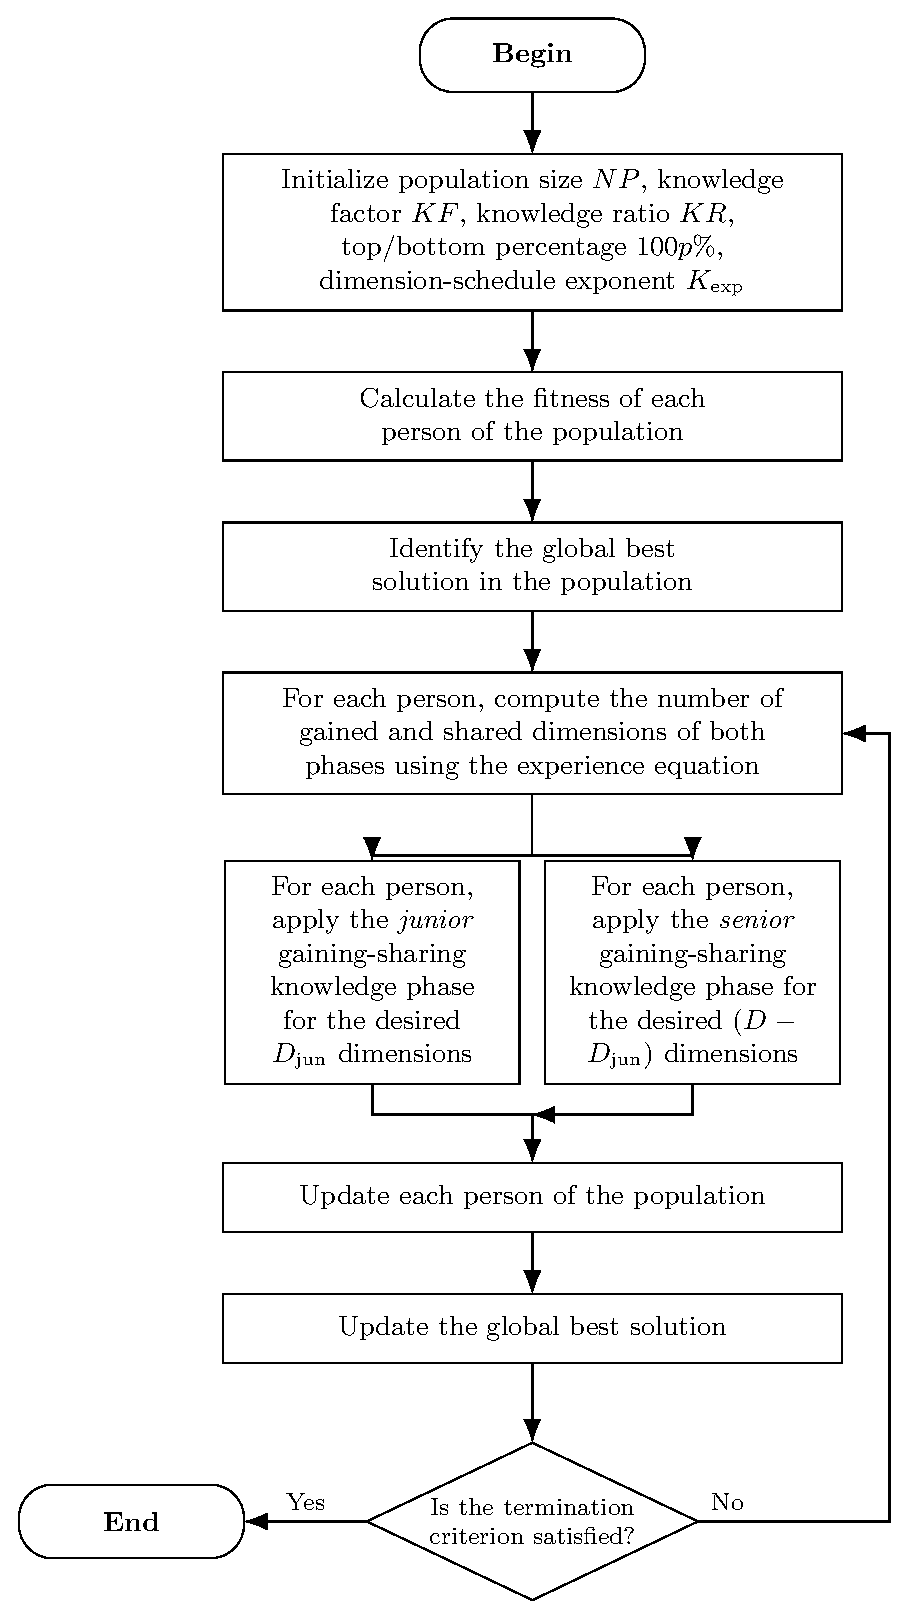
\includegraphics[width=0.62\textwidth]{figures/concept/fig_gsk_flowchart.docx.png}
\caption{@@FIGCAP!fig:gsk-flowchart@@ Flowchart of the base GSK algorithm of Mohamed et
al.~@@CITE!mohamed2020gaining@@, redrawn here from that paper's description: a
single generation loop of
fitness evaluation, gained--shared dimension counting, the junior and senior
gaining-sharing knowledge phases, and greedy update, repeated until the
termination criterion is met. The figure depicts prior work and contributes
nothing new; it is included so the \dtgsk{} flowchart in
Figure~@@REF!fig:dtgsk-flowchart@@ can be read against its parent.}
\label{fig:gsk-flowchart}
\end{figure}

\begin{figure}[p]
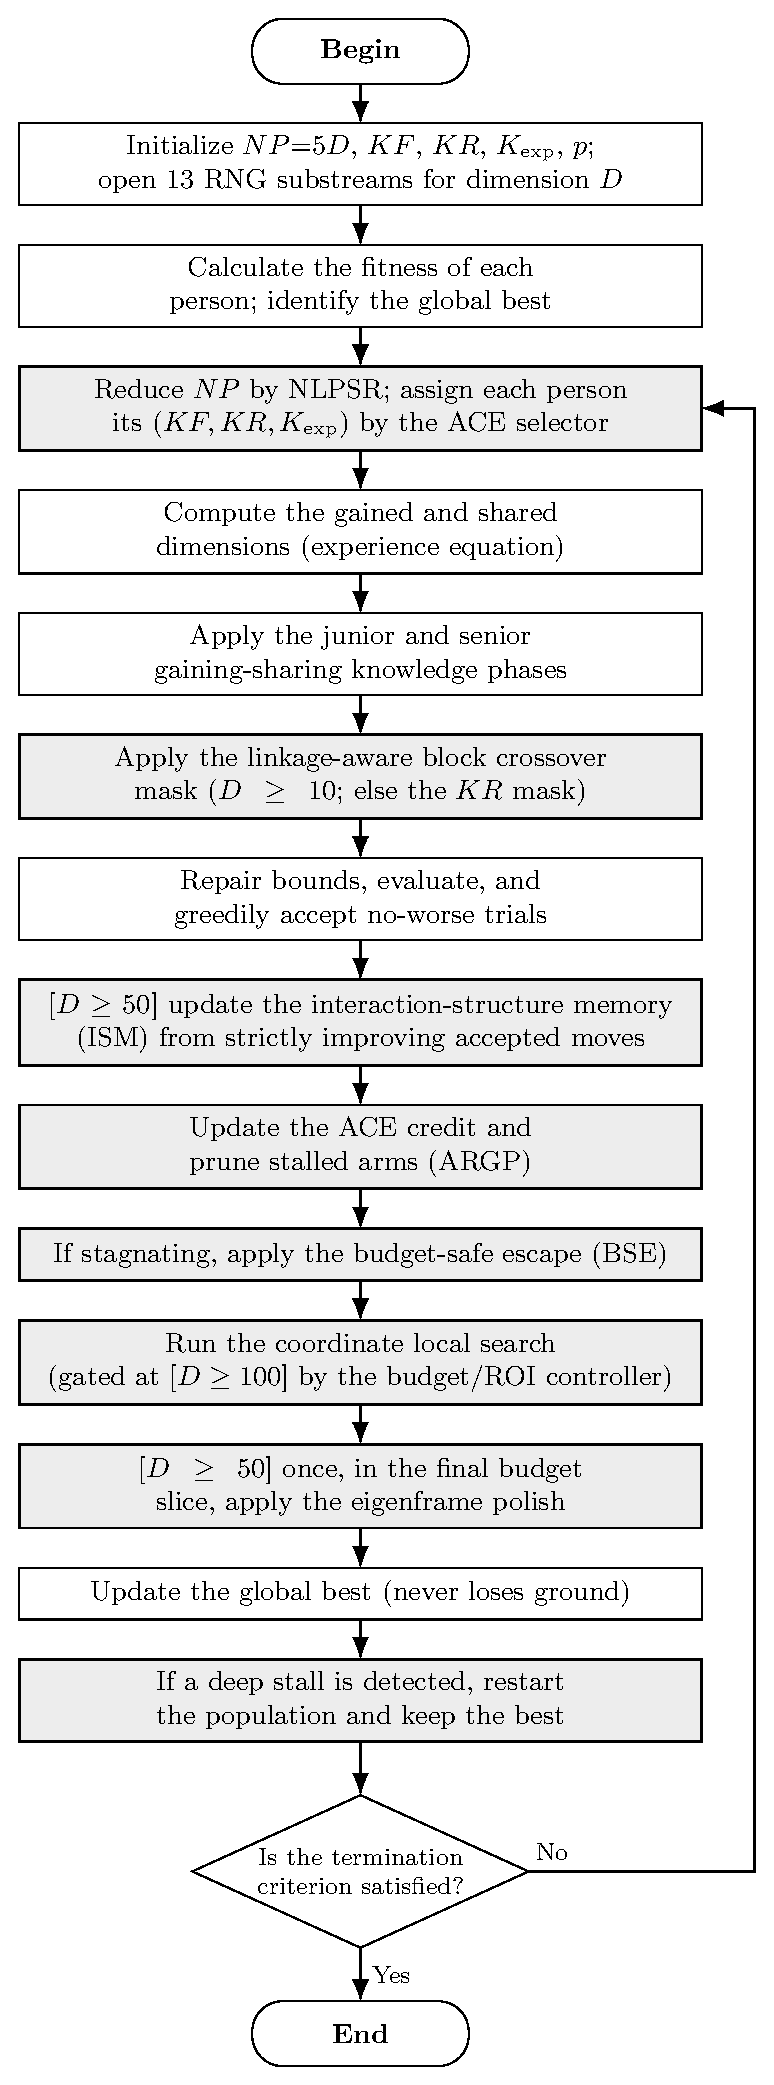
\includegraphics{figures/concept/fig_dtgsk_flowchart.docx.png}
\caption{@@FIGCAP!fig:dtgsk-flowchart@@ Flowchart of the \dtgsk{} algorithm, drawn in the same style as
Figure~@@REF!fig:gsk-flowchart@@ for direct comparison. The GSK core (fitness
evaluation, dimension counting, the junior and senior phases, and the update) is
retained; the boxes with a \textbf{light shaded fill} are the mechanisms \dtgsk{}
adds: the nonlinear population-size reduction (NLPSR) and the ACE selector with
acceptance-gated pruning, the linkage-aware block crossover, the dimension-gated
interaction-structure memory, the coordinate local search, the
budget-safe escape with deep-stall restart,
and the one-shot eigenframe final polish. At $D\ge100$ the upper-tier controllers are cross-cutting rather than a single stage --- they act within the population-reduction, trial-construction, acceptance, and escape steps above (and gate the local search) --- so they are not drawn as a separate node. The global best is preserved
throughout.}
\label{fig:dtgsk-flowchart}
\end{figure}

Within one generation the subsystems execute in the fixed order below,
which Algorithm~@@REF!alg:dt-gsk@@ lists and
Figure~@@REF!fig:dtgsk-flowchart@@ charts.
\begin{enumerate}[noitemsep,topsep=2pt,leftmargin=*,label=(\arabic*)]
\item Nonlinear Population-Size Reduction (NLPSR).
\item Operator-arm sampling by the Adaptive Control Engine (ACE).
\item Junior/senior trial construction and crossover masking.
\item Bound repair and evaluation.
\item Elitist acceptance and the diversity-archive update.
\item At $D\ge50$, the interaction-graph (ISM) update from strictly improving accepted moves.
\item The operator-credit update and Acceptance-Rate Gated Pruning (ARGP)
of the operator pool.
\item Stagnation escape by the Budget-Safe Escape (BSE) mechanism.
\item The charged coordinate local search.
\item At $D\ge50$, the one-shot eigenframe final polish in the final
budget slice.
\item Global-best update.
\item The deep-stall restart check.
\end{enumerate}
The $D\ge100$ upper-tier controllers do not form a separate step in this order: they are cross-cutting, acting within population reduction (the subspace-sampling floor), trial construction (frozen-streak broaden and late linkage random-mix), acceptance (the late-acceptance clip and the basin-memory update), and the budget-safe escape (basin-novelty reseed); a budget/ROI gate additionally gates the local search (a matching hook exists on the escape but never blocks it in the frozen configuration).

A step written ``\textbf{if} $D\ge d$'' in Algorithm~@@REF!alg:dt-gsk@@ is
inactive below tier~$d$. Every subsystem is elitist with respect to the
working population --- it cannot return a population whose best is worse
than the incumbent it was given --- with one deliberate exception: the
deep-stall restart resamples the working population outright
(Section~@@REF!sec:alg:deepstall@@). The global best $x^{gb}$ is held
separately from the working population, is never re-initialized, and is
what the run returns; it therefore never loses ground.

Dimension-tier gating is stated once and holds everywhere.
The blockwise linkage mask is active from $D\ge10$, applied to a
tier-dependent fraction of the population, with the remainder keeping
the per-coordinate $KR$ mask of Eq.~(@@REF!eq:kr-mask@@).
The interaction-structure memory and the
eigenframe final polish activate at $D\ge50$, while the coordinate local search
is active at all tiers. The protective
controllers activate at $D\ge100$. 
Below its tier, each gated block is a no-op.
Table~@@REF!tab:dim-gating@@ gives the activation pattern.



\begin{table}[t]
\caption{@@TABLECAP!tab:dim-gating@@ Subsystem activation across the frozen configuration's four
dimension tiers ($D<20$, $20$--$49$, $50$--$99$, $D\geq100$; the CEC benchmark
dimensions $10/30/50/100$ are the respective tier representatives).
\emph{on}/\emph{off} give the activation state per tier and the last column the
tier-varying parameters. The threshold structure follows the frozen parameter
table (Table~@@REF!tab:parameters@@). Within the $D{<}20$ tier the linkage mask
carries its own $D\geq10$ gate (Table~@@REF!tab:architecture@@), so it is
additionally inactive at the CEC2020 $D=5$ cells.}
\label{tab:dim-gating}
\footnotesize
\zebra
\begin{tabular}{p{3.2cm}cccc p{3.9cm}}
\toprule
\textbf{Subsystem (Eq.)} & \textbf{$D{<}20$} & \textbf{$20$--$49$} & \textbf{$50$--$99$} & \textbf{$D{\ge}100$} & \textbf{Key parameters (by tier)} \\
\midrule
Inherited GSK core (Eqs.~(@@REF!eq:junior-idx@@)--(@@REF!eq:gsk-update@@), (@@REF!eq:midpoint-repair@@); (@@REF!eq:kr-mask@@), (@@REF!eq:greedy-accept@@) as modified) & on & on & on & on & senior $p$ $0.05$ ($0.15$ at $20$--$49$), split-bottom $0.10$ at $D{\ge}50$ \\
NLPSR schedule (Eq.~(@@REF!eq:nlpsr@@)) & on & on & on & on & floor $N_{\min}$ $12$, then $25$ at $D{\ge}50$ \\
ACE selector + ARGP (Eq.~(@@REF!eq:ace-update@@)) & on & on & on & on & single memory, then top/bottom at $D{\ge}20$; DE arm on for $20{\le}D{<}100$ \\
Linkage block crossover (Eq.~(@@REF!eq:kr-mask@@)) & on & on & on & on & block $5$, then $10$; mix $0.70/0.40/0.70/0.70$; ISM-fed blocks at $D{\ge}50$ \\
ISM memory (Eq.~(@@REF!eq:sgsm-graph@@)) & off & off & on & on & $\lambda{=}0.95$, gate $\kappa_{\min}{=}0.35$ (adaptive) \\
Local search (coordinate) & on & on & on & on & axis-aligned; charged; ISM-subspace variant off \\
BSE escape (Eq.~(@@REF!eq:bse-cauchy@@)) + archive & on & on & on & on & $r_{c}$ $0.10$; $r_{\mathrm{rst}}$ $0.30$ then $0.10$; $R_{\max}$ $4/2/4/2$ by tier \\
Upper-tier controllers & off & off & off & on & basin memory, subspace floor, late-accept clip, frozen-broaden, linkage random-mix \\
Eigenframe polish (Eq.~(@@REF!eq:eigen-polish@@)) & off & off & on & on & one-shot, start $0.96$ \\
Deep-stall restart & on & on & on & on & fraction $0.25$; global best preserved \\
\bottomrule
\end{tabular}
\end{table}


\subsection{@@SECNUM!sec:alg:scaffold!3.3.@@ Dimension-Tiered Adaptive Scaffold (Contribution C2)}\label{sec:alg:scaffold}


The scaffold answers a control and budget problem: a single frozen
configuration must remain usable from $D=10$ to $D=100$ without
per-problem tuning, under a greedy selection rule (a trial replaces its
parent when no worse, $\le$; Eq.~(@@REF!eq:greedy-accept@@)) that can
starve the search of accepted moves.
Its five sub-mechanisms are labeled honestly: ACE, NLPSR, BSE, the
diversity archive, and the deep-stall restart are modifications of cited
antecedents; we did not find ARGP's acceptance-rate-gated arm-freezing
rule among the surveyed GSK variants.
The individual contribution of the scaffold subsystems is examined in a
remove-one component study in the Supplementary Materials (with
the interaction-structure memory held off in every cell); ARGP, the final
polish and the deep-stall restart are pre-specified exclusions from that study
and are therefore not isolated. A direct isolation
of the memory overlay itself is reported in the Supplementary Materials
(Section~S6.5) and finds no significant standalone benefit at the
memory's active tiers. The dimension-tiering itself --- resolving control
by dimension rather than at a single fixed operating point --- is likewise
not isolated by a controlled uniform-versus-tiered contrast; C2 is therefore
claimed as the performance of the integrated frozen scaffold as a package,
not as evidence that dimension-tiering is individually causal. Here each
mechanism is specified with its trigger,
timing, and cost. Table~@@REF!tab:notation-scaffold@@ lists the symbols this
subsection introduces.

















\begin{table}[t]
\caption{@@TABLECAP!tab:notation-scaffold@@ Scaffold notation (Contribution C2): symbols for the ACE/ARGP
operator controllers (Sections~@@REF!sec:alg:ace@@--@@REF!sec:alg:argp@@), the
tier-floored population schedule (Section~@@REF!sec:alg:nlpsr@@), and the
budget-safe escape, diversity archive, and restart machinery
(Sections~@@REF!sec:alg:bse@@--@@REF!sec:alg:deepstall@@). Constants take the
frozen-configuration values (Table~@@REF!tab:parameters@@).}
\label{tab:notation-scaffold}
\footnotesize
\begin{tabular}{@{}l@{\hspace{1.2em}}p{0.62\textwidth}@{}}
\toprule
\textbf{Symbol} & \textbf{Meaning}\\
\midrule
\multicolumn{2}{l}{\emph{ACE / ARGP}}\\
\midrule
$\mathcal{A}=\{a_m=(KF_m,KR_m,K_{\exp,m})\}_{m=1}^{M}$ &
  ACE arm pool ($M\in\{5,6\}$; arm 3 = GSK-pure); the optional 6th arm is the DE/rand/1 operator, active at $20{\le}D{<}100$\\
$\pi_m$ & ACE selection probability of arm $m$ (EMA state)\\
$d_m$ & arm-$m$ aggregate improvement $\sum_{i:s_i=m}(f(x_i){-}f(v_i))$ this generation\\
$\tau_m$ & improving-arm normalized share (EMA target for $\pi$)\\
$c=0.10$ & ACE learning rate\\
$\pi_{\min}=0.05$ & ACE probability floor\\
$W_{\text{argp}}=30$ & ARGP acceptance window\\
$\tau_{\text{argp}}$ & ARGP prune threshold ($0.02$ / $0.010$ tier)\\
\midrule
\multicolumn{2}{l}{\emph{NLPSR}}\\
\midrule
$NP(x)=NP_{\text{init}}+(N_{\min}-NP_{\text{init}})\,x^{(1-x)}$ &
  tier-floored nonlinear reduction (rounded half-up)\\
\midrule
\multicolumn{2}{l}{\emph{BSE / archive / restart}}\\
\midrule
$W$ & BSE stagnation window\\
$\epsilon=10^{-8}$ & scale-aware stagnation tolerance\\
$r_{c}=0.10$ & BSE Cauchy-perturbation fraction\\
$r_{\text{rst}}$ & BSE restart (archive-reseed) fraction ($0.30$ low-$D$, $0.10$ otherwise; see Table~@@REF!tab:parameters@@)\\
$R_{\max}$ & maximum BSE restarts ($4/2/4/2$ by tier)\\
$\mathcal{C}(0,1)$ & standard Cauchy draws; rescue scale $\gamma=r_s(u{-}\ell)/\sqrt{D}$ ($r_s$ tier-dependent)\\
$A$ & distance-filtered diversity archive ($|A| = 200$ fixed; L2 admit/replace threshold 0.05; no fitness gate)\\
$\rho_{\text{ds}}=0.25$ & deep-stall frozen-fraction trigger\\
\bottomrule
\end{tabular}
\end{table}




\subsubsection{@@SECNUM!sec:alg:ace!3.3.1.@@ ACE: Bandit Control of the Operator Pool}\label{sec:alg:ace}

A fixed $(KF, KR, K_{\exp})$ triple that suits one landscape or one
dimension tier is brittle on another.
AGSK adapts $KF/KR$ from a fixed pool by success
history~@@CITE!mohamed2020agsk@@, and APGSK widens the adapted parameter
pools~@@CITE!apgsk2021@@; both adapt at the parameter level.



ACE instead adapts at the operator level: it maintains a pool of five complete $(KF, KR, K_{\exp})$
operator settings (a sixth, optional differential-evolution arm joins at
the mid-dimension tiers, below) --- arm~3 is the GSK-pure setting $(0.5, 0.9, 10)$
--- and draws one arm per individual per generation. 
Each arm's per-generation reward is its \emph{aggregate fitness
improvement} $d_m$ --- the summed $f(x_i){-}f(v_i)$ over the individuals
that drew it, not a raw acceptance count. The credit target $\tau$ is mixed
by an exponential moving average at learning rate $c=0.10$ (frozen default)
into the selection-probability vector $\pi$, which is projected onto the
floored simplex $\pi_m\ge\pi_{\min}=0.05$, Eq.~(@@REF!eq:ace-update@@). When the
generation improves in aggregate ($S>0$) the target is the full-pool share
$d/S$. When it does not, the target is restricted to the arms that
individually improved. When no arm improves --- or the aggregate is
exactly zero --- $\pi$ is held unchanged apart from that projection. The floor keeps every arm alive for exploration, and the
improvement-weighted update is in the spirit of SHADE's success
history~@@CITE!tanabe2013shade@@. 
At $D\ge20$ the credit assignment splits into a top/bottom improvement
memory, and for $20{\le}D{<}100$ an optional differential-evolution arm
joins the pool~@@CITE!storn1997differential@@. 
The bandit literature grounds this framing of operator selection as a
dynamic exploration--exploitation
problem~@@CITE!auer2002finite,fialho2010adaptive@@; ACE is not an
instance of those algorithms, and no regret bound is claimed for it.
ACE is control-plane only: it consumes no objective evaluations, and
its per-generation cost is $O(NP + m)$ for $m\in\{5,6\}$ arms (five, or six
with the optional mid-tier DE arm). 

\subsubsection{@@SECNUM!sec:alg:argp!3.3.2.@@ ARGP: Acceptance-Rate Gated Pruning}\label{sec:alg:argp}

The probability floor that keeps ACE exploring also forces draws of
arms that have stopped producing accepted moves.
ARGP resolves this. After a warm-up of 0.15 of
the budget, any arm whose acceptance rate over a rolling window of
$W_{\text{argp}}=30$ generations falls below the tier threshold
$\tau_{\text{argp}}$ (0.02, tightened to 0.010 at $D\ge50$) is
\emph{soft-frozen} to the probability floor $\pi_{\min}=0.05$ rather than removed,
provided at least two arms remain active. Subsequent draws therefore
concentrate on productive operators.  The freeze is recoverable: a frozen arm is re-activated
as soon as its windowed acceptance climbs back to $\tau_{\text{argp}}$, so ARGP
redistributes operator budget rather than permanently retiring it. 
Its bookkeeping cost is $O(m\cdot W_{\text{argp}})$ per
generation. 

\subsubsection{@@SECNUM!sec:alg:nlpsr!3.3.3.@@ NLPSR: Tier-Floored Population-Size Reduction}\label{sec:alg:nlpsr}

NLPSR is explicitly not claimed as new. It keeps the concave $x^{(1-x)}$
reduction shape of APGSK's NLPSR schedule~@@CITE!apgsk2021@@ and
modifies its endpoints, starting from the dimension-scaled
$NP_{\text{init}}=5D$ and bottoming at a tier-specific floor
$N_{\min}$ (25 at $D\ge50$, 12 below) rather than a fixed minimum,
Eq.~(@@REF!eq:nlpsr@@). Each generation the worst surplus rows are
culled. 
The tier floor is the modification that preserves enough parallel
samples for the structure memory at upper tier while letting low
tiers shrink further.
Table~@@REF!tab:worked-example@@ hand-checks the two schedules at
$D=50$.




\begin{table}[H]
\caption{@@TABLECAP!tab:worked-example@@ Worked numeric example at $D=50$: the tier-resolved NLPSR
schedule $NP(x)$ of Eq.~(@@REF!eq:nlpsr@@) (with $NP_{\text{init}}=250$,
$N_{\min}=25$; rounded half-up) and the junior-dimension schedule
$D_{\text{jun}}$ of Eq.~(@@REF!eq:kexp-schedule@@) (with
$K_{\exp}=10$), against the consumed budget fraction $x$. Milestones
mark the frozen configuration's gates; all values are analytic
evaluations of the schedule formulas.}
\label{tab:worked-example}
\small
\begin{tabular}{llll}
\toprule
$x$ & $NP(x)$ & $D_{\text{jun}}$ & Milestone at this budget fraction\\
\midrule
0.00 & 250 & 50 & initialization ($NP_{\text{init}}=5D$)\\
0.10 & 222 & 18 & interaction-graph warm-up ends\\
0.25 & 170 & 3  & deep-stall trigger horizon ($\rho_{\text{ds}}=0.25$ of budget frozen)\\
0.50 & 91  & 1  & senior phase dominates (one junior coordinate remains)\\
0.75 & 41  & 1  & ---\\
0.90 & 27  & 1  & deep-stall restarts stop (stop fraction 0.9)\\
1.00 & 25  & 0  & all coordinates senior; $N_{\min}$ reached; polish window opened at $s_{\text{fp}}=0.96$\\
\bottomrule
\end{tabular}
\end{table}




\subsubsection{@@SECNUM!sec:alg:bse!3.3.4.@@ BSE and the Diversity Archive: Budget-Safe Escape}\label{sec:alg:bse}

Greedy selection over a shrinking population can stagnate: no
accepted moves, collapsing diversity, and a flat improvement signal.
BSE monitors these symptoms over a window of $W=50$ generations. At
$D\ge20$ it uses a triple-trigger detector (signal window 10,
scale-aware tolerance $\epsilon=10^{-8}$, acceptance floor 0.10,
diversity floor 0.35); below $D=20$ it falls back to a single
stagnation trigger, for which the acceptance and diversity floors are
inactive. When triggered it first perturbs the
worst $r_{c}$ fraction of the population with heavy-tailed
Cauchy draws, Eq.~(@@REF!eq:bse-cauchy@@); a successful rescue --- one that
lowers the incumbent best --- cancels the restart for that generation, and
only when the rescue fails does BSE then reseed part of the population from
a diversity archive: a Cauchy-rescue-then-partial-restart design in the
external-archive lineage of adaptive differential
evolution~@@CITE!storn1997differential,zhang2009jade,tanabe2013shade@@. 
The archive is a distance-filtered \emph{diversity} store, not a
fitness-ranked elite set. A candidate is admitted only when it is at
least a normalized-L2 distance $0.05$ from every stored point. Once
the store is full ($|A| = 200$ at every dimension in the frozen configuration; the $1.5\,NP_{\text{init}}$ sizing is the fallback used only when no absolute cap is set, and is inert here)
a new admission overwrites the spatially \emph{closest} entry. There is no
fitness-quality admission or eviction criterion. 
The modification that names the mechanism is its budget safety: BSE is
hard-capped by a maximum restart count $R_{\max}$ (4 at $D{<}20$ and
$50{\le}D{<}100$, else 2) and by a stop fraction beyond which it is disabled, so as a
design fact it can never overshoot
MaxFES. 
When it fires, its cost is $O(r_{\text{rst}}\cdot NP\cdot D)$, and its
restart evaluations are charged like any others
(Section~@@REF!sec:alg:complexity@@). 

\subsubsection{@@SECNUM!sec:alg:deepstall!3.3.5.@@ Deep-Stall Restart with the Global-Best Invariant}\label{sec:alg:deepstall}

BSE perturbs within the current basin; a search that is deeply stuck
needs more.
The deep-stall full restart (multi-start) re-initializes the working
population when the incumbent has been frozen for at least
$\rho_{\text{ds}}=0.25$ of the budget, subject to a cooldown
(0.15 of budget) and a stop fraction (0.9). It draws up to
$\min(NP, \text{remaining budget})$ fresh individuals, truncated when little
budget is left, and the resampled points are evaluated through the same budget
as any other trial. A separate
global-best pair $(x^{gb},f^{gb})$ is preserved across restarts and is what
the run returns. 
This yields the restart-never-loses-ground invariant, a design
property of the implementation: no restart can worsen the reported
result, because the global best is never re-initialized.
A minimum-budget guard (20{,}000 evaluations) keeps tiny budgets
inert, so the mechanism cannot perturb short
runs. 


\subsection{@@SECNUM!sec:alg:ism!3.4.@@ Interaction-Structure Memory and Linkage-Aware Exploitation (Supporting Mechanism)}\label{sec:alg:ism}



















\begin{table}[t]
\caption{@@TABLECAP!tab:notation-ism@@ Interaction-structure memory and eigenframe-polish notation
(supporting mechanism, Section~@@REF!sec:alg:ism@@; Contribution~C1,
Section~@@REF!sec:alg:polish@@). Constants take the frozen-configuration values
(Table~@@REF!tab:parameters@@); the graph-confidence functional is detailed in
Supplementary Materials, Section~S5.}
\label{tab:notation-ism}
\footnotesize
\begin{tabular}{@{}l@{\hspace{1.2em}}p{0.62\textwidth}@{}}
\toprule
\textbf{Symbol} & \textbf{Meaning}\\
\midrule
$G_{\mathrm{abs}}\in\mathbb{R}^{D\times D}$ & non-negative magnitude interaction graph (decaying); confidence gate + linkage\\
$G_{\mathrm{signed}}\in\mathbb{R}^{D\times D}$ & signed interaction graph (decaying); eigenframe-polish basis\\
$g_{\mathrm{act}}\in\mathbb{R}^{D}$ & per-dimension self-weight (decaying; LS dim-selection, inactive in the frozen config)\\
$C\in\mathbb{R}^{D\times D}$ & co-occurrence support/count (decaying)\\
$\lambda=0.95$ & interaction decay (EMA)\\
$\eta=1.0$ & interaction learning rate (EMA accumulation)\\
$\kappa_{\min}=0.35$ & interaction confidence gate (adaptive at $D\ge50$)\\
$\operatorname{conf}(G_{\mathrm{abs}})$ & graph confidence (edge density $\times$ magnitude $\times$ support $\times$ stability; $\kappa(\cdot)$, Supplementary Materials, Section~S5)\\
$V$ & eigenbasis of $G_{\mathrm{signed}}$ (polish directions)\\
$s_{\text{fp}}$ & polish start fraction ($0.96$)\\
\bottomrule
\end{tabular}
\end{table}




As established in Section~@@REF!sec:related@@, no cited GSK-family variant
learns or exploits the interaction structure of the moves a run has
already accepted.
Outside the family, structure learning is available, but at a different
cost or mechanism. Differential grouping spends a dedicated offline
budget of objective evaluations, of order $O(n^{2}/m)$, on pairwise
probing before optimization starts~@@CITE!omidvar2014dg@@. Covariance
matrix adaptation learns a full sampling covariance from selected
steps~@@CITE!hansen2001cmaes@@. Eigenvector-based crossover
recomputes the population-covariance eigenbasis every
generation~@@CITE!guo2015eig@@. 
The design observation behind the interaction-structure memory is that greedy
selection already exposes this signal for free: each accepted move
records which coordinate pairs moved together on an improving step, and
reading that record consumes none of the run's evaluation budget.

The interaction-structure memory accumulates
this evidence in a decaying $D\times D$ interaction graph, updated
only from strictly-improving accepted-move deltas at learning rate $\eta=1.0$.
The retained graph is decayed by $\lambda=0.95$ at each update so that stale
evidence fades, Eq.~(@@REF!eq:sgsm-graph@@). There $\Delta x_i$ is the
accepted move of individual $i$, contributed as an improvement-weighted,
per-move $\ell_1$-normalized outer product. Two of the four state components, the co-evolving interaction
matrices, share this decay--accumulate form; both are symmetrized with a zero
diagonal. A non-negative \emph{magnitude} graph $G_{\mathrm{abs}}$ (built from
$|\Delta x_i|$) supplies the confidence gate $\operatorname{conf}(G_{\mathrm{abs}})$
and the linkage blocks. A \emph{signed} graph $G_{\mathrm{signed}}$
(built from the raw $\Delta x_i$) supplies the eigenframe-polish basis of
Section~@@REF!sec:alg:polish@@. The
full per-move weighting, normalization, and support bookkeeping are in the
Supplementary Materials (Section~S5). Because the graph is allocated only at
$D\ge50$, the operative confidence gate there is $\kappa_{\min}=0.35$,
superseded by an adaptive rolling-window median of recent confidences,
floored at $0.12$; a block is used only when
$\operatorname{conf}(G_{\mathrm{abs}})\ge\kappa_{\min}$. 
The graph is updated every generation and its linkage blocks are
re-extracted every 5 generations --- at $D\ge100$, every 10 and 20
generations respectively --- after a warm-up of 0.10 of the
budget. 
Formally, $G_{\mathrm{signed}}$ is a signed, decaying second-moment (co-movement)
statistic over coordinate \emph{indices}: it is covariance-like in
construction, and the terminal polish of
Section~@@REF!sec:alg:polish@@ operates on its eigenbasis --- a
covariance-eigenbasis operation. The novelty is therefore not that the
learned object is of a fundamentally new type. It is that the object is
accumulated only from strictly-improving accepted moves --- ties and DE-arm
moves are excluded, and local-search moves enter at weight $0.25$ --- then held
signed and decaying, and exploited discretely through block masks and the polish
eigenbasis, all while the GSK vector-update numerics are left unchanged. The
interaction memory records which coordinate indices co-move on improving steps;
it is not a recovered map of the objective's true variable interactions.

ISM consumes no extra objective evaluations, since it observes moves the
run already evaluated. It is not free of cost, however. At $D \geq 50$ each
generation costs $O(D^{2})$ to decay the graph, plus $O(k\,D^{2})$ to
accumulate the $k$ strictly-improving accepted-move outer products ($k \leq NP$).
It also stores four decaying accumulators: the two $O(D^{2})$ interaction
matrices (magnitude $G_{\mathrm{abs}}$ and signed $G_{\mathrm{signed}}$), the
$O(D^{2})$ co-occurrence support $C$, and the $O(D)$ per-dimension activity
$g_{\mathrm{act}}$
(Section~@@REF!sec:alg:complexity@@). 

The learned structure is exploited through two active channels
(Table~@@REF!tab:sgsm-mechanism@@): the linkage-aware block crossover and,
terminally, the eigenframe polish of Section~@@REF!sec:alg:polish@@. A third
channel --- an ISM-block subspace local search --- is implemented but not
enabled in the frozen configuration.
The first active channel is the linkage-aware block crossover. For a
tier-dependent fraction of the population --- about $70\%$ at $D\ge50$ and
$40\%$ at $20$--$49$ --- the per-coordinate $KR$ mask of
Eq.~(@@REF!eq:kr-mask@@) is replaced by a linkage-block mask that copies a
whole block together. The mask is
refreshed every 20 generations ($D{<}50$) or 10 ($D\ge50$). 
The blocks are \emph{not} contiguous coordinate ranges: the random groups
are permutation chunks (arbitrary index subsets) and the ISM-supplied groups
are learned graph components.
Below $D=50$ the blocks are random groups of size 5 --- a
variant of the inherited mask, not a claimed contribution. From
$D\ge50$ each blockwise row draws its blocks from the learned ISM graph
with probability $0.5$, and from the random permutation partition
otherwise (block size 10), so the learned structure supplies about half
of the blockwise rows rather than all of them.
The graph itself is active only for $D\ge50$ and is rebuilt every 5
generations at $D=50$ and every 20 at $D=100$. 
The graph's top-$k$ blocks could \emph{also} define a bounded subspace (at
most 20 coordinates) for a structure-aware local search, but this ISM-block
subspace variant is \emph{not enabled} in the frozen configuration, which
runs a charged axis-aligned coordinate local search instead (the second
active channel, the eigenframe polish, is Section~@@REF!sec:alg:polish@@). Either
way the local-search probes are charged through the normal budget path. 

ISM activates at $D\ge50$ under the frozen configuration; below that
tier no $D\times D$ structure is allocated and \dtgsk{} runs the
adaptive scaffold alone, a structural design fact of the
dimension gating. 
The four-dimensional contrast against the closest structure-learning
lines --- online accepted-move updates, no extra objective evaluations,
a soft decaying pair graph rather than a hard partition or a full
sampling covariance, and discrete exploitation --- is developed in
Section~@@REF!sec:rel:structure@@ and not repeated here.
As stated there, ISM is not claimed to recover the objective's true
separability structure, to confer rotational invariance, or to extend
to large-scale global optimization beyond the dimensions evaluated.



\begin{table}[t]
\caption{@@TABLECAP!tab:sgsm-mechanism@@ How strictly improving accepted moves become exploitable structure:
strictly improving acceptance events update the interaction-structure
memory (ISM) graph EMA (Eq.~(@@REF!eq:sgsm-graph@@)), whose confidence-gated
blocks feed the linkage crossover mask (Eq.~(@@REF!eq:kr-mask@@)), while the
signed graph feeds the eigenframe final polish (Eq.~(@@REF!eq:eigen-polish@@))
directly (without the confidence gate).
The graph is updated continuously from strictly improving accepted moves; the
polish fires once. Eligibility is exactly: only strictly positive improvements
update the ISM (a non-improving move, $\Delta \le 0$, does not; this is the
graph's own strict-positivity gate, not the $10^{-8}$ win/tie/loss reporting
band); DE-arm moves have update weight $0$ in the frozen profile; and
successful local-search displacements enter at weight $0.25$.
No measured interaction structure is shown.}
\label{tab:sgsm-mechanism}
\footnotesize
\begin{tabular}{p{2.4cm}p{7.6cm}p{3.7cm}}
\toprule
\textbf{Stage} & \textbf{What happens} & \textbf{Key detail} \\
\midrule
1. Learn & Strictly improving accepted-move deltas $\Delta x$ update the graph; rejected trials and ties do not. & Improvement signal only; zero extra objective evaluations. \\
2. Memory (Eq.~(@@REF!eq:sgsm-graph@@)) & Two co-evolving accumulators --- a magnitude graph $G_{\mathrm{abs}}$ and a signed graph $G_{\mathrm{signed}}$ --- share $G_\bullet \gets \lambda G_\bullet + \eta\,\operatorname{outer}(\phi_\bullet(\Delta x))$, with $\lambda{=}0.95$, $\eta{=}1.0$. & The linkage-crossover consumer acts only when the magnitude-graph confidence $\operatorname{conf}(G_{\mathrm{abs}})\ge\kappa_{\min}$; the eigenframe polish reads $G_{\mathrm{signed}}$ and fires on any non-zero signed signal (no confidence gate). \\
3. Exploit (two active channels) & (i)~magnitude-graph linkage blocks $\to$ block crossover mask (Eq.~(@@REF!eq:kr-mask@@)); (ii)~signed graph $\to$ eigenbasis $\to$ eigenframe final polish (Eq.~(@@REF!eq:eigen-polish@@)). An ISM-block \emph{subspace} local search is implemented but not enabled (the frozen configuration runs a coordinate local search). & Four-part state ($G_{\mathrm{abs}}$, $G_{\mathrm{signed}}$, support $C$, activity $g_{\mathrm{act}}$): the magnitude graph feeds the crossover mask, the signed graph feeds the polish; the polish fires once, in the final budget slice. \\
\bottomrule
\end{tabular}
\end{table}


\subsection{@@SECNUM!sec:alg:polish!3.5.@@ Eigenframe Final Polish (Contribution C1)}\label{sec:alg:polish}


At the end of a budget-limited run, the incumbent typically sits near
a local minimizer that the population operators refine slowly; a
direct-search endgame is a natural refinement step.
Classical pattern and compass search iterate in the coordinate frame
with a run length that is not bounded a
priori~@@CITE!kolda2003directsearch@@, and the Nelder--Mead simplex, the
common derivative-free default, has documented failure modes and
degrades with
dimension~@@CITE!nelder1965simplex,kolda2003directsearch,gao2012implementing@@.
These properties motivate a capped, deterministic design; they are not
evidence about the polish itself.

The eigenframe final polish is a one-shot deterministic compass search
executed on the eigenbasis $V$ of the ISM signed interaction matrix,
Eq.~(@@REF!eq:eigen-polish@@), falling back to the coordinate axes when
the graph carries no signal.
It fires at most once, in the final budget slice
($s_{\text{fp}}=0.96$ of the budget), and only at $D\ge50$,
where the graph exists. 
Two properties define it.
First, it is RNG-free but not evaluation-free. It draws no random
numbers, so the random-number substreams --- and hence the run up to
the final budget slice --- are byte-identical whether it fires or not.
Every compass probe it then makes is an objective evaluation charged
through the strict budget path, so the polish can never exceed
MaxFES. 
It operates on the working incumbent, re-materialized atomically from the current
population best at the moment it fires, so the incumbent vector and its fitness
always refer to the same individual. A probe is accepted only if strictly
better, so the stage never returns a
point worse than the incumbent and cannot corrupt any reported result. Any out-of-bounds probe component here is repaired by a hard clip to the violated bound (an element-wise projection onto $[\ell_j,u_j]$), not by the parent-and-bound midpoint of Eq.~(@@REF!eq:midpoint-repair@@) used for the junior/senior and DE trials, matching the standard feasibility rule for a bound-constrained direct search.
Second, its basis is drawn from the interaction-structure memory's accepted-move
record rather than from the coordinate frame. Whether this learned basis
outperforms coordinate axes is not established at $D\le100$: the direct
isolation of Supplementary Materials Section~S6.5 cannot separate them.
Any effect that isolation measures therefore attaches to the deterministic,
budget-exact compass endgame as a whole, not to the learned directions.
Its one-time cost is the $O(D^{3})$ eigendecomposition of the
$D\times D$ matrix, incurred once per run
(Section~@@REF!sec:alg:complexity@@). 
The comparison to direct search is conceptual only; no
generating-set-search convergence guarantee is transferred to the
polish or to \dtgsk{}.


\subsection{@@SECNUM!sec:alg:highd!3.6.@@ Upper-Tier Controllers ($D\ge100$)}\label{sec:alg:highd}


At $D\ge100$, the frozen configuration enables a set of protective
controllers documented here as method detail under contribution C2's
dimension-tier scope, not as headline contributions: a late-acceptance
clip, a frozen-streak broadening, a late linkage random-mix, a bounded
basin memory, and a subspace-sampling floor. 
They are scalar guards and bounded memories that protect the late
budget phase of the upper-tier ($D{\ge}100$) runs: clipping late acceptance
drift, broadening after frozen streaks, randomizing a fraction of
linkage assignments, remembering visited basins by spatial novelty, and
keeping a floor on subspace sampling. All are gated to
$D\ge100$ and are no-ops below that tier.
A trust-region displacement governor from earlier development was
\emph{removed} from the code at the paper freeze (it was runtime-dead: its
enable flag was always false, and its clip-rate telemetry is pinned at zero).
A linkage-reliability/predicted-value admission gate remains present in the
codebase as an optional component but is never instantiated by the frozen
configuration. Neither affects any reported trajectory and neither is claimed
as an active mechanism.
Their aggregate per-generation cost is $O(NP\cdot D)$, with the basin
memory bounded at $O(64\cdot D)$. 


\subsection{@@SECNUM!sec:alg:profile!3.7.@@ Parameter Configuration, Determinism, and Configuration Lock (Contribution C3)}\label{sec:alg:profile}


Table~@@REF!tab:parameters@@ consolidates \dtgsk{}'s tier-resolved
configuration, hash-frozen in the repository's freeze manifest and
enforced by unit tests, so the pseudocode, the prose above, and the
executed configuration cannot drift apart; the finer $D\ge100$
controller scalars are pinned in the same frozen manifest.
Where a value varies by tier, the table shows all four tiers; nothing
is tuned per suite or per run on the four bound-constrained suites. On
CEC2013LSGO alone, two linkage-block-size entries are added for
$D = 905$ and $D = 1000$ --- native dimensions outside the shipped tier
table --- set to the benchmark's declared group size of 50 rather than
fitted to any observed result; the rule, its rationale, and its timing
are disclosed in Supplementary Section~S7.























\begin{table}[t]
\caption{@@TABLECAP!tab:parameters@@ Frozen run parameters of the shipped configuration (core).
Where a value varies by dimension tier, the tier-resolved values are given
inline against the four tiers $D{<}20$ / $20$--$49$ / $50$--$99$ / ${\ge}100$.
No tuning is required or permitted at run time.}
\label{tab:parameters}
\small
\begin{tabular}{lll}
\toprule
\textbf{Parameter} & \textbf{Value} & \textbf{Notes}\\
\midrule
\multicolumn{3}{l}{\emph{Run-level (supplied by the benchmark problem and run options)}}\\
\midrule
generator & threefry, unified shared seed & seed policy\\
MaxFES & suite-dependent (Section~@@REF!sec:alg:complexity@@) & $10^4 D$ on CEC2017/CEC2013\\
bounds & uniform scalar $(\ell,u)$ & per-coordinate on CEC2011\\
$NP_{\text{init}}$ & $5D$ & population multiplier 5\\
\midrule
\multicolumn{3}{l}{\emph{Core GSK operator}}\\
\midrule
$KF$ & 0.5 (ACE arm-controlled) & default 0.5\\
$KR$ & 0.9 (ACE arm-controlled) & block mask when linkage on\\
$K_{\exp}$ & 10 (ACE arm-controlled) & junior-dimension schedule\\
$p$ (senior) & 0.05 ($0.15$ at $20$--$49$; split-bottom $0.10$ at $D\ge50$) & \\
\midrule
\multicolumn{3}{l}{\emph{NLPSR}}\\
\midrule
schedule & nonlinear $x^{(1-x)}$ & \\
$N_{\min}$ & 25 at $D\ge50$; 12 below that tier & tier floor\\
$\alpha_{\text{psr}}$ & 1.0 & power-schedule exponent; inert (nlpsr shipped)\\
\bottomrule
\end{tabular}

\vspace{2pt}
{\footnotesize Per-subsystem constants (ACE/ARGP, linkage crossover,
BSE/archive/deep-stall, ISM and the eigenframe polish, and the upper-tier
controllers) are listed in the Supplementary Materials, Section~S5. The
full configuration is hash-frozen in the repository's algorithm freeze
manifest.}
\end{table}




Table~@@REF!tab:panel@@ records the comparator panel and its
configuration provenance.
All seven algorithms are run in-repository under one frozen protocol;
the six comparators run their published reference constants, and eGSK
is the Python port in which the SciPy SLSQP solver substitutes the
published MATLAB fmincon polish --- the panel column is
therefore ``eGSK (Python port, SLSQP polish)'', with no
numerical-equivalence claim between the two
backends. 


\begin{table}[H]
\caption{@@TABLECAP!tab:panel@@ GSK-family panel roster and configuration provenance.
All panel results are produced by in-repository
re-runs under one frozen protocol (identical evaluator, budgets,
seeds, and shared initial populations; the \dtgsk{} self-init
exception is documented in the experimental setup). No
literature-copied numbers appear in any panel exhibit.}
\label{tab:panel}
\small
\begin{tabular}{lll}
\toprule
\textbf{Algorithm} & \textbf{Reference} & \textbf{Configuration in this study}\\
\midrule
GSK & @@CITE!mohamed2020gaining@@ & reference-implementation constants, $NP=100$ at every $D$; in-repository re-run\\
AGSK & @@CITE!mohamed2020agsk@@ & reference-implementation constants, $NP=100$ at every $D$; in-repository re-run\\
APGSK & @@CITE!apgsk2021@@ & reference-implementation constants, $NP=100$ at every $D$; in-repository re-run\\


FDB-AGSK & @@CITE!fdbagsk2023@@ & reference-implementation constants, $NP=100$ at every $D$; in-repository re-run\\
ATMALS-GSK & @@CITE!alfadli2025atmals@@ & reference-implementation constants, $NP=100$ at every $D$; in-repository re-run\\
eGSK & @@CITE!jawad2024egsk@@ & Python port; SLSQP substitutes the published
fmincon polish (disclosed)\\
\dtgsk{} & this paper & frozen tier-resolved configuration
(Table~@@REF!tab:parameters@@); hash-locked\\
\bottomrule
\end{tabular}
\end{table}



The exact numeric settings behind ``published constants'' are reproduced
in Table~@@REF!tab:comparator-params-main@@ so the main text is
parameter-complete without the Supplementary Material: every value is
read programmatically from the shipped optimizer modules --- module
constants imported, runner-visible defaults extracted from source ---
never hand-transcribed, and the frozen campaign configuration records an
empty per-optimizer override set for every comparator, so these module
defaults are the settings of record. Pools are written first:step:last.
\dtgsk{} is omitted from this table because its core frozen
configuration is given in Table~@@REF!tab:parameters@@ (per-subsystem
constants: Supplementary Material, Section~S5); its single
documented per-suite exception --- the two CEC2013LSGO linkage-block
entries ($905 \to 50$, $1000 \to 50$) --- is disclosed in
Section~@@REF!sec:exp:cec2013lsgo@@ and Supplementary Section~S7.



\begin{table}[H]
\caption{@@TABLECAP!tab:comparator-params-main@@ GSK-family comparator parameter settings exactly as run in this
study, read from the shipped optimizer modules. Identical settings apply
on all five suites; no comparator is tuned per suite. Bracketed lists are
per-arm pools; ranges are written first:step:last.}\label{tab:comparator-params-main}


\begin{tabular}{@{}l p{11.4cm}@{}}
\toprule
\textbf{Algorithm} & \textbf{Parameter settings as run} \\
\midrule
GSK & NP = 100; Kf = 0.5; Kr = 0.9; K = 10.0; p = 0.1 \\
AGSK & NPinit = 100; NPmin = 12; Kf pool = [0.1, 1, 0.5, 1]; Kr pool = [0.2, 0.1, 0.9, 0.9]; Kw init = [0.85, 0.05, 0.05, 0.05]; p = 0.05 \\
APGSK & NPinit = 100; NPmin = 12; Kf pool = [0.1, 1, 0.5, 1]; Kf pool (neg.) = [-0.15, -0.05, -0.05, -0.15]; Kr pool = [0.2, 0.1, 0.9, 0.9]; Kw init = [0.85, 0.05, 0.05, 0.05]; p = 0.05 \\
FDB-AGSK & NPinit = 100; NPmin = 12; FDB case = 1; Kf pool = [0.1, 1, 0.5, 1]; Kr pool = [0.2, 0.1, 0.9, 0.9]; p = 0.05 \\
ATMALS-GSK & NP = 100; Kf pool = 0.2:0.1:0.8 (7 values); Kr pool = 0.85:0.01:1 (16 values); K pool = 8:1:30 (23 values); p pool = 0.05:0.01:0.15 (11 values); PLS pool = 1:0.1:2 (11 values) \\
eGSK & NP = 100; Kf1, Kf2 = 0.5; Kr = 1; K = 10; p = 0.1; late-stage frac. = 0.75; IP budget frac. = 0.002 \\
\bottomrule
\end{tabular}



\end{table}

Determinism is contribution C3's core.
A 13-substream, append-only, prefix-locked counter-based random-number
layer child-seeds every subsystem from one run seed,
Eq.~(@@REF!eq:rng-substreams@@), where substream $k$ is derived by
counter-based child-seeding and substream 0 is the run seed
verbatim. 
Because each subsystem draws from its own named substream --- with a
few closely related mechanisms, such as the deep-stall restart, sharing
the budget-safe-escape substream --- toggling a subsystem cannot
disturb the draw order of any subsystem on a different substream. Three
distinct reproducibility levels should be kept apart. The first is
\emph{RNG-substream isolation}: the structural guarantee just stated, which
makes component-level re-evaluation well defined and is test-enforced in the
repository's regression suite. The second is \emph{same-environment trajectory
repeatability}: bit-for-bit identical runs under the same single-threaded
build with a fixed floating-point reduction order, which is the shipped
configuration. That is not a cross-thread or cross-platform guarantee, as noted
in Section~@@REF!sec:experiments@@. The third is \emph{artifact byte-identity}:
the released result files reproduce byte-for-byte after the documented
normalization. All three cover \dtgsk{} and this repository's pipeline only;
no byte-stability claim is made for the comparator implementations.


\subsection{@@SECNUM!sec:alg:complexity!3.8.@@ Complexity and Evaluation Accounting}\label{sec:alg:complexity}


\paragraph{Computational cost.}
Per generation, the scaffold costs what the base algorithm costs:
trial construction, masking, and bound repair are $O(NP\cdot D)$,
ranking is $O(NP\log NP)$, ACE and ARGP add $O(NP+M)$ and
$O(M\cdot W_{\text{argp}})$ bookkeeping, and the archive update is an
$O(|A|\cdot D)$ distance check. 
The dimension-gated structures dominate only at upper tier. The three
$O(D^{2})$ interaction matrices are decayed at $O(D^{2})$ per update, the
$O(D)$ activity vector at $O(D)$, and each
strictly-improving accepted move contributes a rank-one outer product over
its active-coordinate set $J$ ($O(|J|^{2})$, $|J|\le D$); this sums to
$O(NP\cdot D^{2})$ worst case, and less when the per-move support is sparse.
That update runs every generation at $D=50$--$99$, but is thinned at $D\ge100$
to every tenth generation from a capped sample of accepted moves, with its
linkage blocks re-extracted on a slower multi-generation cadence. The
eigenframe polish performs a single $O(D^{3})$ eigendecomposition once per
run. 
For $D<50$ no $D^{2}$ or $D^{3}$ interaction structure is allocated. The
sub-$20$ tier is $O(NP\cdot D)$ per generation like GSK. At $20\le D<50$ the
only added term is the optional DE arm's vectorized donor selection: a partial
selection over an $n_{\mathrm{DE}}\times NP$ key matrix, $O(n_{\mathrm{DE}}\cdot NP)$
with a matching transient buffer (up to $O(NP^{2})$ when most rows draw DE).
That is bounded compute, not budget. 
Memory is dominated by the $O(NP\cdot D)$ population family at every tier ---
the population, trial, and three-buffer RNG workspaces, all $\Theta(NP\cdot D)$
with $NP_{\text{init}}=5D$ --- which at $D=100$ is on the order of a few
megabytes in float64.  The dimension-gated interaction state adds three
persistent $O(D^{2})$ matrices (magnitude $G_{\mathrm{abs}}$, signed
$G_{\mathrm{signed}}$, and co-occurrence support $C$), an $O(D)$ activity vector,
and several reusable $O(D^{2})$ scratch buffers. That is about half a megabyte at
$D=100$ --- a minority of the live footprint even where it is largest. Alongside
it sit the diversity archive ($\le 200\cdot D$) and the one-shot $O(D^{2})$
eigenframe workspace. 
We claim no complexity improvement over GSK: the $D^{2}/D^{3}$ terms
are bounded compute overhead --- not budget --- paid for
zero-extra-objective-evaluation structure learning, and the
dimension gating means low-dimensional runs pay none of it.
Measured wall-clock overhead is reported with the experimental
results.

\paragraph{Evaluation accounting.}
Every objective evaluation flows through a single
budget controller holding the evaluation budget MaxFES ($10^{4}D$ for
CEC2017 and CEC2013, $150{,}000$ for CEC2011, $5\times10^{4}$,
$10^{6}$, $3\times10^{6}$ and $10^{7}$ at $D = 5/10/15/20$ for CEC2020,
and $3\times10^{6}$ for CEC2013LSGO); there is
no second counter and no path that calls the objective
directly. 
This includes every evaluation spent by the coordinate local search, the
BSE rescue, the deep-stall re-initialization, and the polish probes
--- none is exempt.
When a final batch would exceed the remaining budget, only the prefix
that fits is evaluated and charged, so runs are MaxFES-exact by
construction: budget-exact, monotone, and repeat-identical, as
verified by the repository's deterministic
trace. 
One protocol exception is disclosed here and documented in the
experimental setup: \dtgsk{} self-initializes, drawing its own
$5D$-point initial population from the same seed-paired stream as the
shared runner-generated initial populations, rather than consuming the
runner's matrix; the draw is deterministic and charged like any
other. 






\section{@@SECNUM!sec:experiments!4.@@ Experimental Study}\label{sec:experiments}






On CEC2017 \dtgsk{} attains the best overall Friedman
mean rank in the seven-algorithm panel, placing first at three of four
dimensions and second at $D = 30$; on CEC2011 it is likewise second, with
a Holm-significant loss to \egsk{}. The CEC2020 and CEC2013LSGO legs,
added under a registered analysis-plan addendum, are reported in
Sections~@@REF!sec:exp:cec2020@@ and~@@REF!sec:exp:cec2013lsgo@@ at their
registered evidential tiers, and the five-suite synthesis is confined to
Section~@@REF!sec:exp:discussion@@. The evidence below is reported at that
resolution --- tier by tier, with the unfavorable cells stated alongside
the favorable ones --- because the dimension-resolved pattern, not a single
aggregate, is what the dimension-tiered design predicts and what the data
support. Every comparative statement is scoped to this panel; no
field-wide claim is made.


\subsection{@@SECNUM!sec:exp:settings!4.1.@@ Experimental Setup}\label{sec:exp:settings}


\paragraph{Evidence discipline.}
Every empirical value in this paper derives from a versioned, immutable
evidence release: all seven
panel algorithms were re-run in-repository under one identical
protocol, and the analysis pipeline
(SciPy~1.15.3) runs
restricted so that it can read only the three such releases identified in
the Data Availability Statement --- the primary three-suite release and
the two later, separate, non-superseding single-suite releases for
CEC2013LSGO and CEC2020 --- never staging data and never
literature-copied numbers
presented as comparable.

One provenance qualification applies: the \egsk{} panel cells derive
from the committed reference results of the runnable \egsk{} port,
whose late local polish uses SciPy-SLSQP, whereas the original
reference implementation uses a fmincon-based SQP
solver~@@CITE!jawad2024egsk@@. The substituted routine is a search
component rather than a cosmetic finishing step: it consumes part of the
same evaluation budget and can move the returned solution, so the \egsk{}
cells reported here are properties of this port and not of the published
implementation. Cross-implementation runtime and environment comparability
is therefore limited, no runtime-superiority claim is made anywhere in this
paper, and no claim of numerical equivalence to the published \egsk{} is
made in either direction.


\paragraph{Suites, budgets, and metrics.}
Table~@@REF!tab:protocol@@ summarizes the frozen protocol. The primary
suite is the CEC2017 bound-constrained suite~@@CITE!awad2016problem@@:
29 functions (F1, F3--F30) at $D \in \{10, 30, 50, 100\}$, 51 runs per
(function, dimension), $\mathrm{MaxFES} = 10^{4} \cdot D$, and final
error $f(\mathbf{x}) - f(\mathbf{x}^{*})$ with errors below $10^{-8}$
treated as zero per the suite's reporting convention. F2 is excluded under the
adopted CEC2017 protocol because of documented instability and
difficult-to-reproduce behavior, uniformly in every panel cell.

The real-world suite is CEC2011~@@CITE!das2011cec2011@@, which supplies
real-world problem \emph{formulations} executed as a standardized benchmark:
22 problems at their native dimensions, 25 runs per problem,
$\mathrm{MaxFES} = 150{,}000$. This is breadth of application formulation,
not evidence of deployment performance. The endpoint is the raw best objective
value, and negative optima occur on some problems. The error column
is NaN by design on problems without published optima, where
best-fitness is authoritative.
Infeasible evaluations --- for instance a failed trajectory integration
or an out-of-domain intermediate value on the orbital-mechanics problems
--- receive the suite's standard infeasibility penalty ($10^{30}$),
applied identically for all seven algorithms, so a feasible candidate is
always preferred to an infeasible one at selection.

Finally, CEC2013~@@CITE!liang2013cec2013@@ is reported as a second
comparison suite for breadth of comparison under the same protocol:
28 functions at $D \in \{10, 30, 50\}$, 51 runs,
$\mathrm{MaxFES} = 10^{4} \cdot D$, same error convention.

Two further suites were added after the primary release under a
registered analysis-plan addendum, with their protocol facts fixed at
registration. The CEC2020 bound-constrained suite~@@CITE!yue2020cec2020@@
is the pre-registered \emph{confirmatory} suite: 10 functions at
$D \in \{5, 10, 15, 20\}$, with F6 and F7 undefined at $D = 5$, giving
38 protocol cells; 30 runs per cell; a dimension-dependent budget of
$\mathrm{MaxFES} = 5 \times 10^{4}$, $10^{6}$, $3 \times 10^{6}$, and
$10^{7}$ at $D = 5/10/15/20$; and the same error basis and $10^{-8}$
floor as CEC2017.

The CEC2013LSGO large-scale suite~@@CITE!li2013lsgo@@ --- distinct from
the bound-constrained CEC2013 suite above --- is the post-hoc,
\emph{family-internal} suite: 15 functions at their native $D = 1000$
(F13 and F14 at 905 through their overlap), 25 runs,
$\mathrm{MaxFES} = 3 \times 10^{6}$, and the raw best-objective basis
(the error column is not populated on this suite). Its F3, F6 and F10
were executed with the transformed Ackley variant, so results on those
three functions are not comparable to published values obtained on the
raw variant, and no such comparison is drawn anywhere in this paper.


\begin{table}[H]
\caption{@@TABLECAP!tab:protocol@@ Frozen evaluation protocol, one row per suite. The seed schedule is
optimizer-independent
and keyed by (dimension, function, run); the full-schedule
recomputation audit for the primary release (70{,}813 rows, 0 mismatches) is
part of the
released evaluation record, and the CEC2020 and CEC2013LSGO banks were
audited for cross-algorithm seed identity at promotion (0 mismatches).
CEC2020 scores 38 protocol cells (F6 and F7 are undefined at $D = 5$);
CEC2013LSGO runs F13 and F14 at their native $D = 905$.}\label{tab:protocol}
\setlength{\tabcolsep}{4pt}
\begin{tabular}{lccccc}
\toprule
\textbf{Suite} & \textbf{Problems} & \textbf{Dimensions} & \textbf{Runs} & \textbf{MaxFES} & \textbf{Endpoint} \\
\midrule
CEC2017 (primary) & 29 (F1, F3--F30) & 10/30/50/100 & 51 & $10^{4}\cdot D$ & error ($<10^{-8}\!\to\!0$) \\
CEC2011 (real-world) & 22 & native & 25 & $150{,}000$ & raw best objective \\
CEC2013 (second comparison) & 28 (F1--F28) & 10/30/50 & 51 & $10^{4}\cdot D$ & error ($<10^{-8}\!\to\!0$) \\


CEC2020 (confirmatory) & 10 & 5/10/15/20 & 30 & $5{\cdot}10^{4}/10^{6}/3{\cdot}10^{6}/10^{7}$ & error ($<10^{-8}\!\to\!0$) \\
CEC2013LSGO (family-internal) & 15 & 1000 (F13/F14: 905) & 25 & $3\times10^{6}$ & raw best objective \\
\midrule
Seed schedule & \multicolumn{5}{c}{$s(D,f,r) = (20240620 + 1000003\,D + 1000033\,f + 1000037\,r) \bmod (2^{31}{-}2) + 1$} \\
Generator & \multicolumn{5}{c}{counter-based Threefry; identical schedule for all seven optimizers on every suite} \\
Initialization & \multicolumn{5}{c}{runner-generated shared $X_{0}$; exception: \dtgsk{} self-init from the same stream} \\
Significance & \multicolumn{5}{c}{$\alpha = 0.05$; Holm at $m{=}6$ per dimension (across-function layer); tie band $|\Delta| < 10^{-8}$} \\
\bottomrule
\end{tabular}

\end{table}

\paragraph{Panel, pairing, and seed-paired start.}
The comparison panel is exactly the seven-algorithm GSK family of
Table~@@REF!tab:panel@@; comparator configurations follow their original
publications, and \dtgsk{} runs the single hash-frozen configuration
(Table~@@REF!tab:parameters@@), identical across the four bound-constrained
suites with no per-suite tuning. On CEC2013LSGO alone it adds two
linkage-block-size entries, for $D = 905$ and $D = 1000$, set to the
benchmark's own declared group size of 50 rather than fitted to any
observed result; without them the shipped table falls back to a block
size of 10. The values were added while LSGO results already existed, so
outcome-blindness is not asserted for them; the rule, the rationale, and
the timing are disclosed in Supplementary Section~S7.

That configuration was, however,
selected on CEC2017, which is therefore the \emph{development} suite and is
selection-exposed; CEC2011 and CEC2013 were not consulted during
configuration selection and serve as \emph{corroborative} suites, not
independent development benchmarks; CEC2020 is the \emph{pre-registered
confirmatory} suite, whose analysis plan, hypotheses and outcome wording
were committed before any CEC2020 result existed; and CEC2013LSGO is
\emph{post-hoc exploratory} and family-internal, its descriptive layer
having been inspected before registration. The CEC2017 standing should
accordingly be
read as development-suite performance, the CEC2011/CEC2013 standings as
corroboration, the CEC2020 standing as the registered confirmatory test,
and the CEC2013LSGO standing as exploratory. Six full-panel candidate
configurations, including the one
selected, were compared against the seven-algorithm panel on CEC2017 before
promotion; the full development protocol and the scope of that count are
disclosed in the Supplementary Materials, Section~S5.

Runs are paired across optimizers by common seed, problem instance, and
run index: within each suite all seven optimizers use the identical seed
schedule of Table~@@REF!tab:protocol@@ on byte-identical problem instances.

For the six comparators, run $r$ additionally starts from the same
runner-generated initial population $X_{0}$; \dtgsk{} is the one
documented exception --- it self-initializes its own $5 \cdot D$ population
from the same seed-paired random stream, so its initial population is drawn
under the identical seed but is \emph{not} byte-identical to the shared
$X_{0}$. Pairing is therefore by common seed/problem/run rather than by an
identical starting population for \dtgsk{}; the exception is recorded in
the protocol exhibit and the pairing audit rather than hidden.

One evidence gap is disclosed up front. At the time of the frozen analysis,
APGSK per-run records on CEC2017 were available only at $D = 100$, the
result of a sidecar-overwrite anomaly in the evidence tree. Seeds and
summary values for $D \in \{10, 30, 50\}$ were verified equivalent from the
generation logs, so run-level statistics against APGSK at those dimensions
were treated as disclosed-unavailable and were never imputed. The primary
across-function test on per-function means --- the same test used for every
comparator --- still applies to APGSK. Those run-level records were
subsequently recovered and are present in the released bundle; only the
non-deterministic wall-clock runtime remains unavailable at those
dimensions. The recovery was deterministic, from the seed-identical per-run logs, and reproduces the frozen APGSK summaries exactly; because the primary analysis was already frozen when it landed, the manuscript conservatively retains the function-level basis reported here, and no headline number is affected.







\paragraph{Environment and determinism.}
All runs were executed on a 22-logical-core Windows workstation
(Windows 11, build 10.0.26200) under Python~3.10.11 with Numba~0.64.0
JIT kernels. Campaigns parallelize only across independent
(function, dimension, run) cells --- 15 worker processes, with no parallelism
inside a run. Every cell records an environment.json
manifest including the git commit, JIT state, and floating-point
probe hashes of the shared RNG, the \dtgsk{} kernels, and the suite
evaluators. The comparator-specific update kernels are \emph{not} covered
by a numerical probe: their JIT state is recorded, but their numerical
identity across producer commits rests on the shared-kernel probes and code
history rather than on a direct hash.


The analysis bundle records its own environment (NumPy~2.2.6,
SciPy~1.15.3, pandas~2.3.3).

For \dtgsk{}, every objective evaluation, including polish and escape
evaluations, is charged through the strict budget-accounting path
described in Section~@@REF!sec:algorithm@@; the reference-faithful
comparator ports instead retain their original budget-crossing
semantics, evaluating the terminal batch in full and counting only its
in-budget prefix. No optimizer is therefore charged more than
$\mathrm{MaxFES}$; AGSK and APGSK additionally stop on reaching the
$10^{-8}$ target error, which ends $1{,}845$ of the primary evidence
release's $75{,}250$ runs
(AGSK $962$ and APGSK $883$, summed over CEC2017 and CEC2013; by suite,
$742$ and $1{,}103$ respectively) below the cap, while
the remaining five optimizers implement no such criterion and always consume
the full budget. That crossing falls only on the terminal
generation, so the uncounted rows enter no incumbent and no later state.
A controlled cell was constructed so that the budget is not a multiple of the
population, forcing the crossing for every optimizer that exhibits it.
Overwriting all such rows leaves the returned solution, its fitness and the
charged budget bit-identical for all seven. The inertness itself follows
structurally, from the prefix-only incumbent scan and immediate loop exit, so
the crossing confers no search advantage.




Runs are budget-exact and
repeat-identical; byte-identical reproduction at $D \geq 50$ requires
single-threaded numerical kernels (a fixed reduction order), and the
shipped runs use one compute thread per run, so the repeat-identical
property holds for them but is not guaranteed under a different thread
configuration. This determinism is established for \dtgsk{} in its
declared single-threaded environment; it is not claimed for the
comparator ports across producer commits, where a re-execution of the
six comparators was verified \emph{not} to reproduce the frozen
scientific columns exactly (a floating-point path shifted between the
producing commits, amplified on a minority of runs by the chaotic
search). The released evidence is unaffected --- it is the archived
output of the original campaign --- but a bit-identical re-timing of the
comparators under current code is not achievable, which is why the
runtime table is reported for \dtgsk{} only. Per-run raw
CSVs, seed schedules, and verification manifests ship with the
release (see the Data Availability statement).


No generative-AI system contributed to the design, execution, or analysis
of the experiments or to any reported number; a large language model was
used for language editing, the drafting of descriptive prose, and
software-engineering support, as
declared in full in the back matter (Use of Generative Artificial
Intelligence).


\paragraph{Statistical protocol.}
Hypotheses are stated once here. For each comparator and dimension,
a two-sided Wilcoxon signed-rank test~@@CITE!wilcoxon1945individual@@
is applied to the 29 paired per-function mean errors
($H_{0}$: the paired differences are symmetric about zero), with
Holm step-down correction~@@CITE!holm1979simple@@ across the
six simultaneous comparators at that dimension ($\alpha = 0.05$).
Win/tie/loss counts use the tie rule $|\Delta| < 10^{-8}$ --- the same
$10^{-8}$ the suite uses to floor errors to zero, here applied to the
per-function mean difference. This single absolute band is a coarse
convention across functions of very different scales, so the win/tie/loss
tallies are a \emph{descriptive} companion only. The Friedman test ranks
\emph{within} each function and is therefore invariant to per-function scale;
the Wilcoxon signed-rank test, applied here across per-function mean
differences, ranks the absolute differences \emph{across} functions and is
accordingly \emph{not} scale-invariant --- functions with larger numerical
ranges carry more weight in it. The tie band itself affects no significance
decision, but this cross-function scale heterogeneity is a genuine limitation
of the paired test, and is one reason the Friedman ranking is treated as the
primary aggregate. Every
test is accompanied by its \emph{aligned} effect size: because the
across-function test is a matched-pairs Wilcoxon, the tabulated effect size is
the matched-pairs rank-biserial correlation
$r = (R^{+} - R^{-})/(R^{+} + R^{-})$, where $R^{+}$ is the rank sum of the
comparisons favoring \dtgsk{}, so that $r > 0$ favors \dtgsk{}. (The released
workbook stores the same quantity under the mirrored column names
w\_plus/w\_minus, whose roles are exchanged relative to
$R^{+}/R^{-}$. Its rank\_biserial column already carries the sign
convention used here.) The
unpaired Vargha--Delaney $A_{12}$~@@CITE!vargha2000critique@@ ($A_{12} > 0.5$
favors \dtgsk{}; the conventional 0.56/0.64/0.71 guidelines label magnitudes)
is retained as a descriptive companion in the released workbooks. Zero differences under the tie rule
($|\Delta| < 10^{-8}$) are discarded before ranking
(zero\_method=`wilcox'), and the reported $p$-values are produced by
this repository's own pure-\textsc{NumPy} wilcoxon\_paired routine
using the normal approximation with continuity correction. That routine is
cross-checked against scipy.stats.wilcoxon
(zero\_method=`wilcox', correction=True,
method=`approx') in the released cross\_check.json; of the
three audited cells, the two with a defined statistic agree on it to a
relative tolerance of $10^{-12}$ and on the $\alpha = 0.05$ decision, the
third is degenerate (every paired difference inside the tie band) and is
recorded as $p = 1$ by convention, and any disagreement would have failed
the release gate.
The effective post-zero sample sizes are recorded in the released
per-comparison $R^{+}/R^{-}$ workbooks. The released-workbook $A_{12}$ is
computed over the 29 per-function mean errors --- the same unit as the
across-function Wilcoxon --- and is therefore an \emph{unpaired}
distributional effect size, distinct from the run-level Vargha--Delaney
$A_{12}$ in the released effect-size workbook; the 0.56/0.64/0.71
thresholds are applied here as descriptive labels on that function-mean
summary. The released per-comparison workbooks carry $r$ alongside
$R^{+}/R^{-}$ for every comparison, with $A_{12}$ retained as the descriptive
distributional companion.

For the multi-algorithm view, a Friedman
test~@@CITE!friedman1937use@@ with the Iman--Davenport correction~@@CITE!demsar2006statistical@@ is
run per dimension over the per-function mean errors ($H_{0}$: all
seven algorithms have equal mean ranks). Only where the
omnibus is significant does a Nemenyi critical-difference (CD)
analysis~@@CITE!demsar2006statistical@@ follow. It is rendered as mean-rank plots
annotated with the CD reference span rather than the clique-connected
diagram form, and non-separable groups are identified in the text. Bias-corrected
and accelerated (BCa) bootstrap intervals~@@CITE!efron1993introduction@@
accompany the mean ranks ($n_{\mathrm{boot}} = 10{,}000$, seeded); because
they resample each algorithm's \emph{fixed} per-function midranks rather than
re-ranking the algorithms within every bootstrap sample, they are reported as
\emph{descriptive} rank-stability intervals, not inferential rank-uncertainty
intervals.
Dimensions are never pooled into a single test. Decision symbols are
derived mechanically from corrected $p$-values, and $p$-values below
$10^{-4}$ are reported as bounded, never as ``0.0000''. The test statistics are computed by this repository's own analysis module and
validated against scipy.stats (SciPy~1.15.3), which is used directly
only for distribution tails. The Friedman statistic uses the tie-corrected
rank variance that underlies the Iman--Davenport $F$, with scipy.stats
supplying the $F$-distribution tail. The Wilcoxon $p$-values come from the
in-repo wilcoxon\_paired routine (normal approximation with continuity
correction), cross-checked against scipy.stats.wilcoxon as recorded
in the released cross\_check.json. The Nemenyi critical difference uses the tabulated
$q_{0.05}(k = 7) = 2.949$ of~@@CITE!demsar2006statistical@@, not a \textsc{SciPy}
studentized-range call. The correction
is material: the $10^{-8}$ success floor maps distinct outcomes onto
exactly $0$, so exact ties concentrate in the low-dimensional panels
(correction factor $C = 0.890$ at $D = 10$, covering 9 of 29 functions,
and $0.979$ at $D = 30$; $C = 1$ exactly at $D = 50$ and $D = 100$, where
no ties occur). Because $C \le 1$ the correction can only increase the
statistic, and it leaves the mean ranks untouched; every omnibus decision,
rank, and effect direction reported here is identical under the corrected
and uncorrected forms. Both are released per panel in
friedman\_ranks\_*.csv so the correction can be checked directly.

The complete
per-comparison workbooks --- including signed-rank sums $R^{+}$/$R^{-}$
and per-function detail --- are released with the reproducibility bundle
(they accompany the analysis scripts and are not typeset in the supplement).



\subsection{@@SECNUM!sec:exp:cec2017!4.2.@@ Results on the CEC2017 Primary Suite}\label{sec:exp:cec2017}


\subsubsection{@@SECNUM!sec:exp:cec2017:desc!4.2.1.@@ Per-Function Results}\label{sec:exp:cec2017:desc}

The complete per-function tables are provided at every dimension in
Supplementary Materials, Sections~S1 and~S2. Section~S1 carries the
seven-algorithm mean $\pm$ SD panels for \dtgsk{} and all six comparators;
Section~S2 carries the five-statistic detail (best/median/worst/mean/SD over 51
runs) for the \dtgsk{}-versus-GSK head-to-head. The main text carries the panel-level summaries
(Table~@@REF!tab:friedman-cec2017@@) and the inferential statistics
(Table~@@REF!tab:wilcoxon-holm@@) so that the central comparative
claims are auditable without the supplement.
Against the original GSK, \dtgsk{}'s per-function win/tie/loss
records are 22--4--3, 19--2--8, 22--0--7, and 20--0--9 at
$D = 10/30/50/100$.

By function class, the pattern is dimension-dependent. On the hybrid
functions (F11--F20) \dtgsk{} attains the best or equal-best class
mean rank in the panel at $D \geq 30$, scoring 1.60 at $D = 30$ (equal with
\egsk{}), 1.80 at $D = 50$, and 2.30 at $D = 100$ (again equal with \egsk{}).

On the simple multimodal functions (F4--F10) it holds the best
class mean rank at $D \in \{10, 50, 100\}$ (2.07, 2.29, 1.71), but
stands second behind \egsk{} at $D = 30$ (3.29 vs.\ 2.43).

The composition functions (F21--F30) are the least favorable class at
low dimension: at $D = 10$ \dtgsk{}'s class mean rank is 3.70,
behind \apgsk{} (2.65), \fdbagsk{} (2.75), and \agsk{} (2.90),
whereas at $D = 50$ it leads the class (2.50) and at
$D \in \{30, 100\}$ it is second behind \egsk{} (2.85 vs.\ 2.45 and
2.90 vs.\ 2.70).


\subsubsection{@@SECNUM!sec:exp:cec2017:panel!4.2.2.@@ Family-Panel Comparison}\label{sec:exp:cec2017:panel}

Table~@@REF!tab:friedman-cec2017@@ reports the Friedman mean ranks of
the seven-algorithm panel per dimension (its final column gives the
overall aggregate), with the companion per-dimension bar chart in
Figure~@@REF!fig:cec2017-ranks@@; an overall-aggregate bar view and a
rank-versus-dimension trend plot are provided in the Supplementary
Materials. Within the
GSK-family panel, \dtgsk{} attains the best Friedman mean rank at
$D = 10$ (2.88), $D = 50$ (2.21), and $D = 100$ (2.34), and the
second-best at $D = 30$ (2.50), behind \egsk{} (2.29); the
Friedman--Iman--Davenport omnibus is significant at every dimension
($p \leq 1.2 \times 10^{-9}$).

The favorable ranks coexist with losing head-to-head records against
\egsk{}: the per-function win/tie/loss is 11--2--16 at $D = 30$,
13--0--16 at $D = 50$, and 12--0--17 at $D = 100$, so the first
places at $D \geq 50$ are earned by consistency against the whole
panel, not by dominating \egsk{}.

The ``Overall'' column (2.48 for \dtgsk{}, best of 7; \egsk{} second
at 2.96) is the unweighted mean of the four per-dimension Friedman
mean ranks --- a descriptive aggregation with no cross-dimension test
attached. The Iman--Davenport correction applies to each
per-dimension omnibus, not to the overall row.




@@TABLECAP!tab:friedman-cec2017!T16@@ Friedman mean ranks (lower is better) of the seven-algorithm
GSK-family panel on CEC2017 per dimension (the four columns
$D \in \{10, 30, 50, 100\}$; 29 per-function mean
errors as blocks, 51 runs each) plus the unweighted across-dimension
mean (``Overall'', a descriptive aggregate); the Friedman +
Iman--Davenport omnibus is significant at every dimension
($p \leq 1.2 \times 10^{-9}$). Best rank per column in bold. Rank-ordering statements are qualified by
the prespecified robustness battery
(Section~@@REF!sec:exp:stats@@). The \apgsk{} evidence gap and its
consequence for the inferential basis are stated in
Section~@@REF!sec:exp:settings@@.

@@NATIVETABLE!T16@@



\begin{figure}[H]
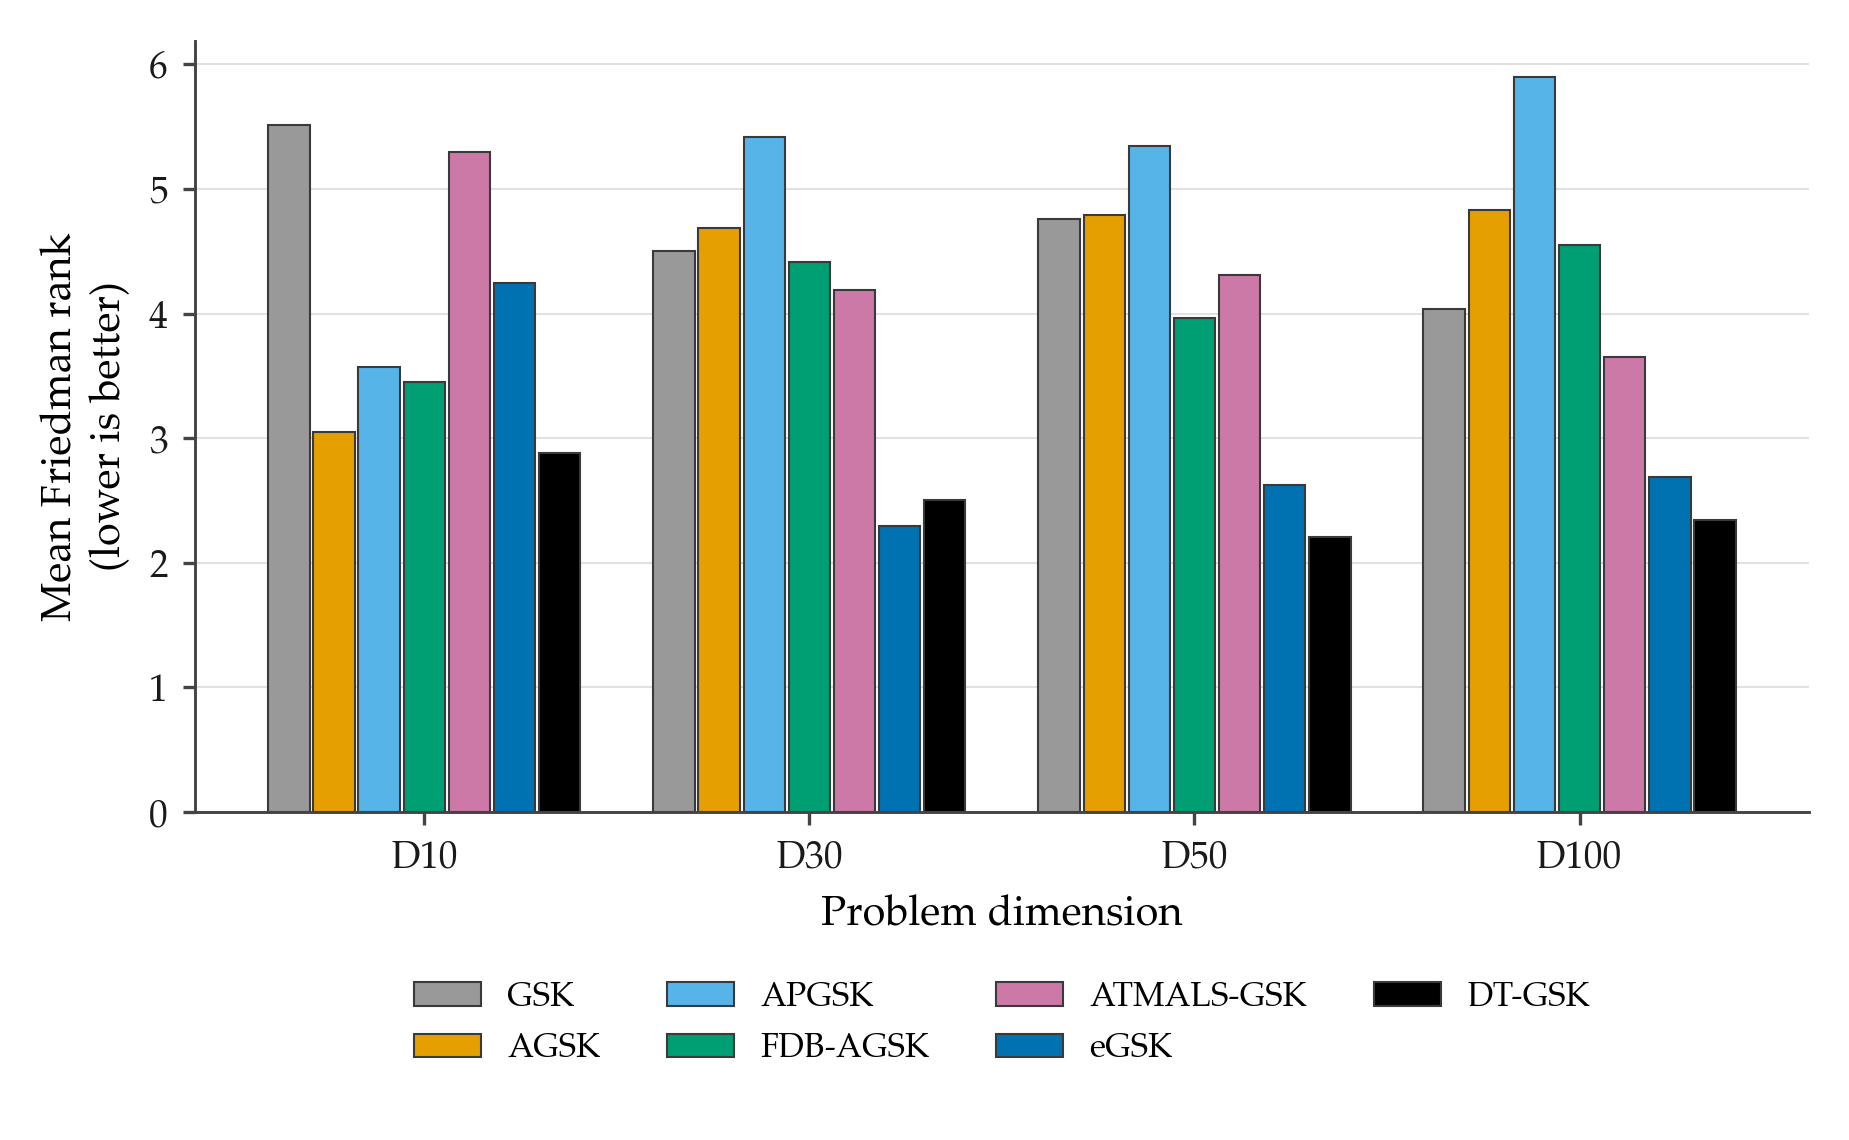
\includegraphics[width=0.75\textwidth]{figures/ranks/cec2017_mean_ranks.png}
\caption{@@FIGCAP!fig:cec2017-ranks@@ Friedman mean ranks per dimension (CEC2017, 29 functions,
51 runs), grouped by dimension in the fixed panel order; companion to
Table~@@REF!tab:friedman-cec2017@@. Lower is better. Rank-robustness and APGSK-gap
qualifications as in Table~@@REF!tab:friedman-cec2017@@.}\label{fig:cec2017-ranks}

\end{figure}

\subsubsection{@@SECNUM!sec:exp:stats!4.2.3.@@ Statistical Analysis}\label{sec:exp:stats}

\paragraph{Statistical protocol.}
Comparisons use the Wilcoxon signed-rank test~@@CITE!wilcoxon1945individual@@ on
paired per-function means, with Holm step-down
correction~@@CITE!holm1979simple@@ applied within each dimension over the family
of six comparators; the tie-corrected Friedman test~@@CITE!friedman1937use@@
supplies mean ranks and Nemenyi critical differences supply the post-hoc
separation~@@CITE!demsar2006statistical@@. In every case the null hypothesis is
that the compared algorithms' error distributions do not differ on the tested
family, and the alternative is that they do; $\alpha = 0.05$ throughout.
An effect size accompanies every test
--- the matched-pairs rank-biserial $r$ here, and BCa bootstrap intervals on the
mean ranks in the Supplementary Materials --- because a $p$-value alone does not
convey magnitude. Two reporting rules follow and are applied throughout. First,
an uncorrected family of per-comparator tests inflates the family-wise error
rate, so no significance claim in this paper rests on an uncorrected
$p$~@@CITE!holm1979simple,demsar2006statistical@@. Second, win/tie/loss counts are
descriptive summaries of per-function outcomes and are never read as
significance: every $\alpha = 0.05$ decision reported here comes from a
Holm-adjusted test, and the two quantities are kept in separate columns so they
cannot be conflated.

Table~@@REF!tab:wilcoxon-holm@@ reports the across-function Wilcoxon
tests with Holm correction, win/tie/loss counts, rank-biserial $r$ effect
sizes, and Holm decisions for \dtgsk{} against each comparator at
each dimension. Two qualifications apply to how that table should be
read. The companion $A_{12}$ summary is computed over the 29 per-function means,
on the same unit as the Wilcoxon test, and is therefore distinct from
the run-level $A_{12}$ reported in the effect-size workbook; the two
are not interchangeable. The \apgsk{} rows at
$D \in \{10, 30, 50\}$ rest on function-level tests over per-function
means, which was the inferential basis available there because \apgsk{}
per-run records were missing at analysis freeze and recovered only
afterwards.




@@TABLECAP!tab:wilcoxon-holm!T15@@ \dtgsk{} vs.\ each GSK-family comparator on CEC2017 (29
functions, 51 runs, per-function mean error), in two aligned sub-tables:
$D \in \{10, 30\}$ above, $D \in \{50, 100\}$ below. Columns are the
across-function Wilcoxon signed-rank $p$ and its Holm-corrected value
(family $= 6$ comparators per dimension, $\alpha = 0.05$), win/tie/loss
counts with tie rule $|\Delta| < 10^{-8}$, the matched-pairs rank-biserial
effect size $r$ ($> 0$ favors \dtgsk{}), and the Holm decision ($+$ better,
$\approx$ no significant difference, $-$ worse).

@@NATIVETABLE!T15@@



Of the 24 Holm-corrected cells (six comparators $\times$ four
dimensions), 17 are significant wins for \dtgsk{}, 7 show no
significant difference, and none is a significant loss. The Holm correction is
applied within each dimension (family size 6), so this 24-cell count aggregates
four independent within-dimension families. It is a descriptive tally,
not a single jointly family-wise-error-controlled result.

As a sensitivity check, applying Holm once across all 24 hypotheses --- the
most conservative reading, in which the four dimensions are treated as a
single family --- leaves 15 of the 24 cells significant. Only two cells do
not survive (\atmals{} at $D = 10$ and GSK at $D = 30$, both
$p_{\mathrm{Holm}}$ just under $0.05$ within their own dimension), and the
count of significant losses remains zero under either correction.

The unfavorable and borderline cells are stated plainly. Against
\egsk{}, \dtgsk{} wins significantly only at $D = 10$
($p_{\mathrm{Holm}} = 0.0035$); at $D \in \{30, 50, 100\}$ the
outcome is not significant ($p_{\mathrm{Holm}} = 0.199$, $1.0$, and $0.795$)
with tabulated rank-biserial $r$ of $-0.286$, $-0.002$, and $-0.057$ ---
negligible magnitudes, all three faintly negative and therefore leaning
marginally toward \egsk{}.

Against GSK, the $D = 100$ cell is not significant after Holm correction
($p_{\mathrm{raw}} = 0.0323$, $p_{\mathrm{Holm}} = 0.0646$) despite a
20--0--9 win/tie/loss record.

At $D = 10$, first place is carried by Holm-significant wins over
GSK, \atmals{}, and \egsk{} only; the cells against \agsk{},
\apgsk{}, and \fdbagsk{} show no significant difference
($p_{\mathrm{Holm}} = 1.0$ each).

At $D \in \{30, 50, 100\}$, \dtgsk{} beats \agsk{}, \apgsk{}, and
\fdbagsk{} in all nine cells ($p_{\mathrm{Holm}} \leq 0.011$) and
\atmals{} at all four dimensions
($p_{\mathrm{Holm}} \leq 0.037$); the largest effect is against
\apgsk{} at $D = 100$ ($r = +0.977$).


Seeded bootstrap BCa rank-stability intervals attached to the Friedman mean ranks
(Supplementary Materials, Section~S2) qualify the rank point estimates. They
resample the fixed per-function midranks rather than recomputing ranks within
each resample, so they are read descriptively as a spread on the mean rank,
never as a formal overlap test. \dtgsk{}'s intervals are [2.29, 3.43], [2.07, 3.10],
[1.86, 2.69], and [1.90, 2.83] at $D = 10/30/50/100$; they overlap
\egsk{}'s intervals at $D \in \{30, 50, 100\}$, consistent with the
pairwise non-significant cells above.




Figure~@@REF!fig:cd-cec2017@@ shows the Nemenyi mean-rank
plots with CD span (one panel per dimension), emitted only because the omnibus is significant at every
dimension; for $k = 7$ algorithms and $N = 29$ functions at
$\alpha = 0.05$, $\mathrm{CD} =
q_{0.05}\sqrt{k(k+1)/(6N)} = 1.67$ rank units
($q_{0.05} = 2.949$).

The plots make one limitation explicit: \dtgsk{} and \egsk{} are
never Nemenyi-separable at any CEC2017 dimension. Their rank gaps
are 1.36, 0.21, 0.41, and 0.34 at $D = 10/30/50/100$ on the unrounded mean
ranks, all inside the CD band. (The $D=100$ gap reads $0.35$ if formed from the
two-decimal displayed ranks.) The per-dimension orderings between these two
algorithms must therefore not be over-read as statistically established
separations.


\begin{figure}[htbp]
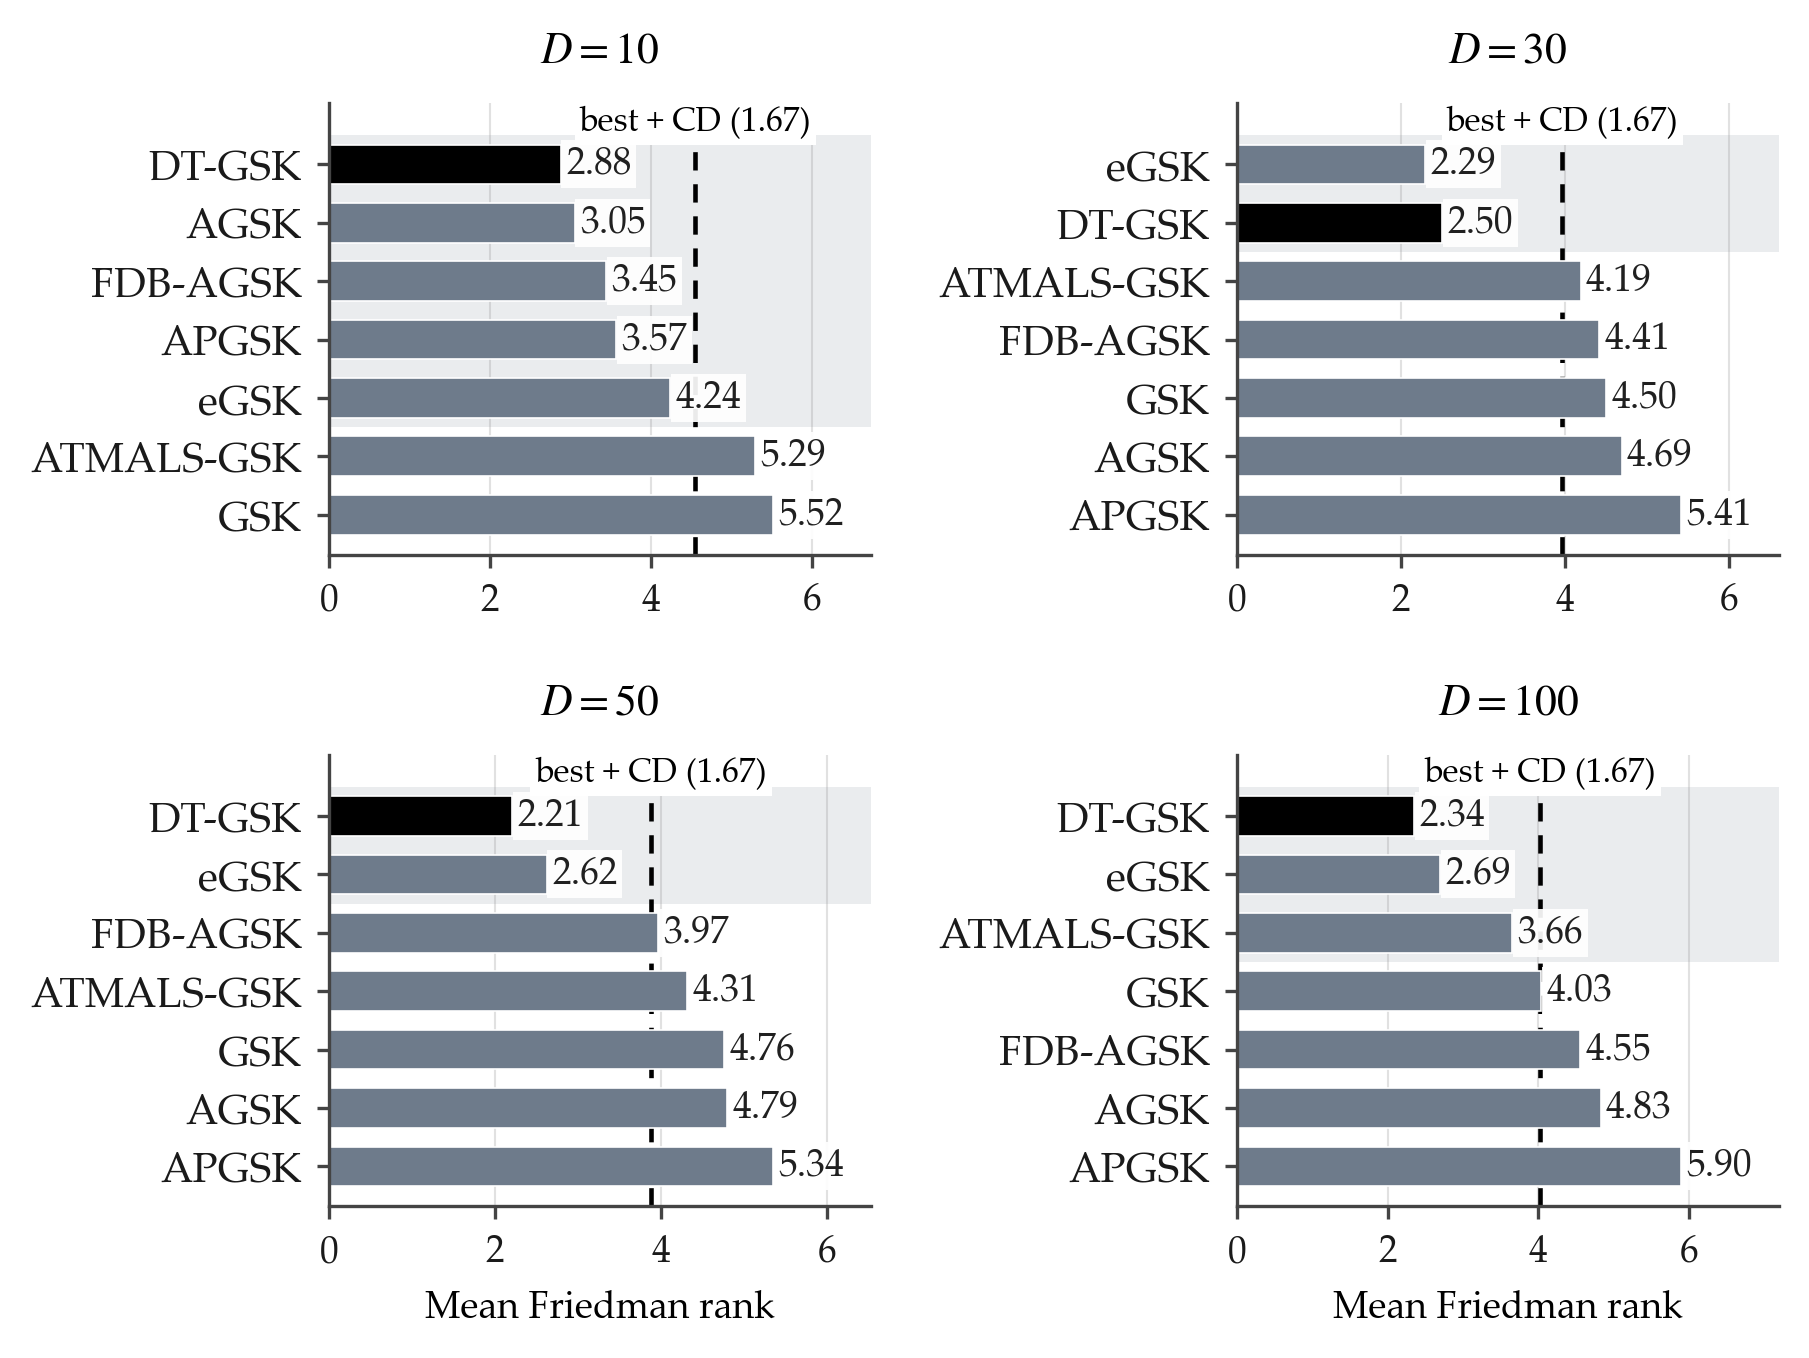
\includegraphics[width=\textwidth]{figures/nemenyi/nemenyi_cd_cec2017_grid.png}
\caption{@@FIGCAP!fig:cd-cec2017@@ Nemenyi mean-rank plots with critical-difference (CD) span for the
CEC2017 GSK-family Friedman mean ranks (lower is better), one panel per
dimension
($D = 10, 30, 50, 100$; $k = 7$, $N = 29$, $\alpha = 0.05$,
$\mathrm{CD} = 1.67$ rank units, $q_{0.05} = 2.949$); emitted only because the
Friedman omnibus is significant at every dimension.  The within-one-CD-of-best
cohort (the algorithms not separated from the best by more than one CD) is
\{\dtgsk{}, \agsk{}, \fdbagsk{}, \apgsk{}, \egsk{}\} at $D{=}10$;
\{\egsk{}, \dtgsk{}\} at $D{=}30$ (best rank \egsk{}); \{\dtgsk{}, \egsk{}\}
at $D{=}50$; and \{\dtgsk{}, \egsk{}, \atmals{}\} at $D{=}100$.  Rank-robustness
and APGSK-gap qualifications as in
Table~@@REF!tab:friedman-cec2017@@.}\label{fig:cd-cec2017}

\end{figure}

The Friedman mean rank improves with dimension overall but is not monotone
across $D \in \{10, 30, 50, 100\}$ --- 2.88, 2.50, 2.21, 2.34 ---: $D = 30$
is an ordinal dip to second place and $D = 100$ is slightly worse than
$D = 50$ (a rank-versus-dimension trend plot is provided in the Supplementary
Materials).


\paragraph{Robustness of the rank statements.}
A prespecified robustness battery accompanies the release, and two
of its checks diverge from the primary analysis and therefore qualify
every rank-ordering statement above. Re-ranking on median (rather
than mean) per-function errors shifts win/tie/loss tallies materially
--- 21--4--4 becomes 17--10--2 against \egsk{} at $D = 10$ --- and
swaps two comparator pairs, \apgsk{}/\egsk{} at $D = 10$ and
\fdbagsk{}/\atmals{} at $D = 50$. Excluding the disputed APGSK cells
at $D \leq 50$ swaps GSK and \fdbagsk{} at $D = 30$.

Mean-based ranks are the prespecified primary; \dtgsk{}'s own
ordinal positions (1/2/1/1 at $D = 10/30/50/100$) are identical in
every variant reported here, but panel orderings between comparators are not fully
robust. Under the median endpoint \dtgsk{}'s $D = 100$ first place becomes
an exact tie with \egsk{} (both 2.59), consistent with their documented
non-separability. As a deliberate pairing-sensitivity check, an unpaired Mann--Whitney companion was also run over the
696 function-by-comparator-by-dimension cells, each a run-level test on 51
paired runs. Dropping the pairing moves 11 cells from significant to
non-significant and 21 in the opposite direction, with no sign reversals. The
robustness criterion (no sign reversals) is met, and the net effect of
dropping the pairing is an increase in significances rather than a
simple power loss --- and an
exploratory Benjamini--Hochberg
companion~@@CITE!benjamini1995controlling@@ over the run-level tests is
included in the released analysis workbooks (which accompany the
reproducibility bundle, not the typeset supplement).
One robustness check is disclosed as a surrogate. Because errors are floored
to zero at write time, raw sub-floor values are unrecoverable from the
release, so the error-floor sensitivity check could not be run on the raw
values. It was executed instead in its pre-registered nearest-admissible form,
with ties handled at the floor and means $\le 10^{-8}$ snapped to zero before
ranking and win/tie/loss. A scan of the 71,400 stored per-run errors found no
value in the open interval $(0, 10^{-8})$, so the surrogate and the raw check
would coincide on this release. The substitution is nonetheless recorded rather
than presented as the check itself.



\subsection{@@SECNUM!sec:exp:cec2011!4.3.@@ Results on the CEC2011 Real-World Suite}\label{sec:exp:cec2011}


The per-problem five-statistic results of \dtgsk{} against the original
GSK on the 22 CEC2011 problems --- together with the \egsk{} loss and the
\dtgsk{}-versus-GSK detail --- are reported in the Supplementary Materials,
Section~S2 (the complete six-comparator across-problem Wilcoxon--Holm
matrix is in the released analysis bundle), and the full convergence grids
in Section~S3. The endpoint is the raw best objective value; error cells
are NaN by design on problems without published optima, and best-fitness
is authoritative there. This suite is corroborative, so the main text
reports its ranking (Figure~@@REF!fig:cec2011-ranks@@) and significance
below and defers the dense per-problem five-statistic table to the
supplement.


Within the GSK-family panel, \dtgsk{} places second of seven on
CEC2011 by Friedman mean rank (3.36), behind \egsk{} (2.52); the
omnibus is significant (Iman--Davenport $F = 4.27$,
$p = 6.0 \times 10^{-4}$), and Figure~@@REF!fig:cec2011-ranks@@ shows
the resulting ordering.

The across-problem Holm-corrected Wilcoxon against \egsk{} is a
statistically significant loss
($p_{\mathrm{raw}} = 9.5 \times 10^{-3}$,
$p_{\mathrm{Holm}} = 4.2 \times 10^{-2}$). It is the single
Holm-significant unfavorable headline cell in this study, and it
accompanies every CEC2011 placement statement in this paper. As on CEC2017,
the \dtgsk{}--\egsk{} Friedman-rank gap of $0.84$ is nonetheless within the
Nemenyi critical difference of $1.92$ here.

The remaining pairwise outcomes at the same family size are two
significant wins --- against \agsk{}
($p_{\mathrm{Holm}} = 1.6 \times 10^{-2}$) and \fdbagsk{}
($p_{\mathrm{Holm}} = 4.2 \times 10^{-2}$) --- and no significant difference against GSK,
\apgsk{} ($p_{\mathrm{Holm}} = 0.137$ each), and \atmals{}
($p_{\mathrm{Holm}} = 0.323$).

The head-to-head against the original GSK illustrates why the suite
is corroborative rather than headline evidence: the descriptive
record favors \dtgsk{} (win/tie/loss 13--2--7,
$R^{+} = 159$ vs.\ $R^{-} = 51$), but the across-problem test does
not survive Holm correction
($p_{\mathrm{raw}} = 4.6 \times 10^{-2}$,
$p_{\mathrm{Holm}} = 0.137$) at $n = 22$ problems.

CEC2011 therefore corroborates within-family competitiveness on
real-world problems at native dimensions --- a competitive placement
(second of seven) --- and does not corroborate first place; no headline
claim in this paper rests on CEC2011 alone.


\begin{figure}[H]
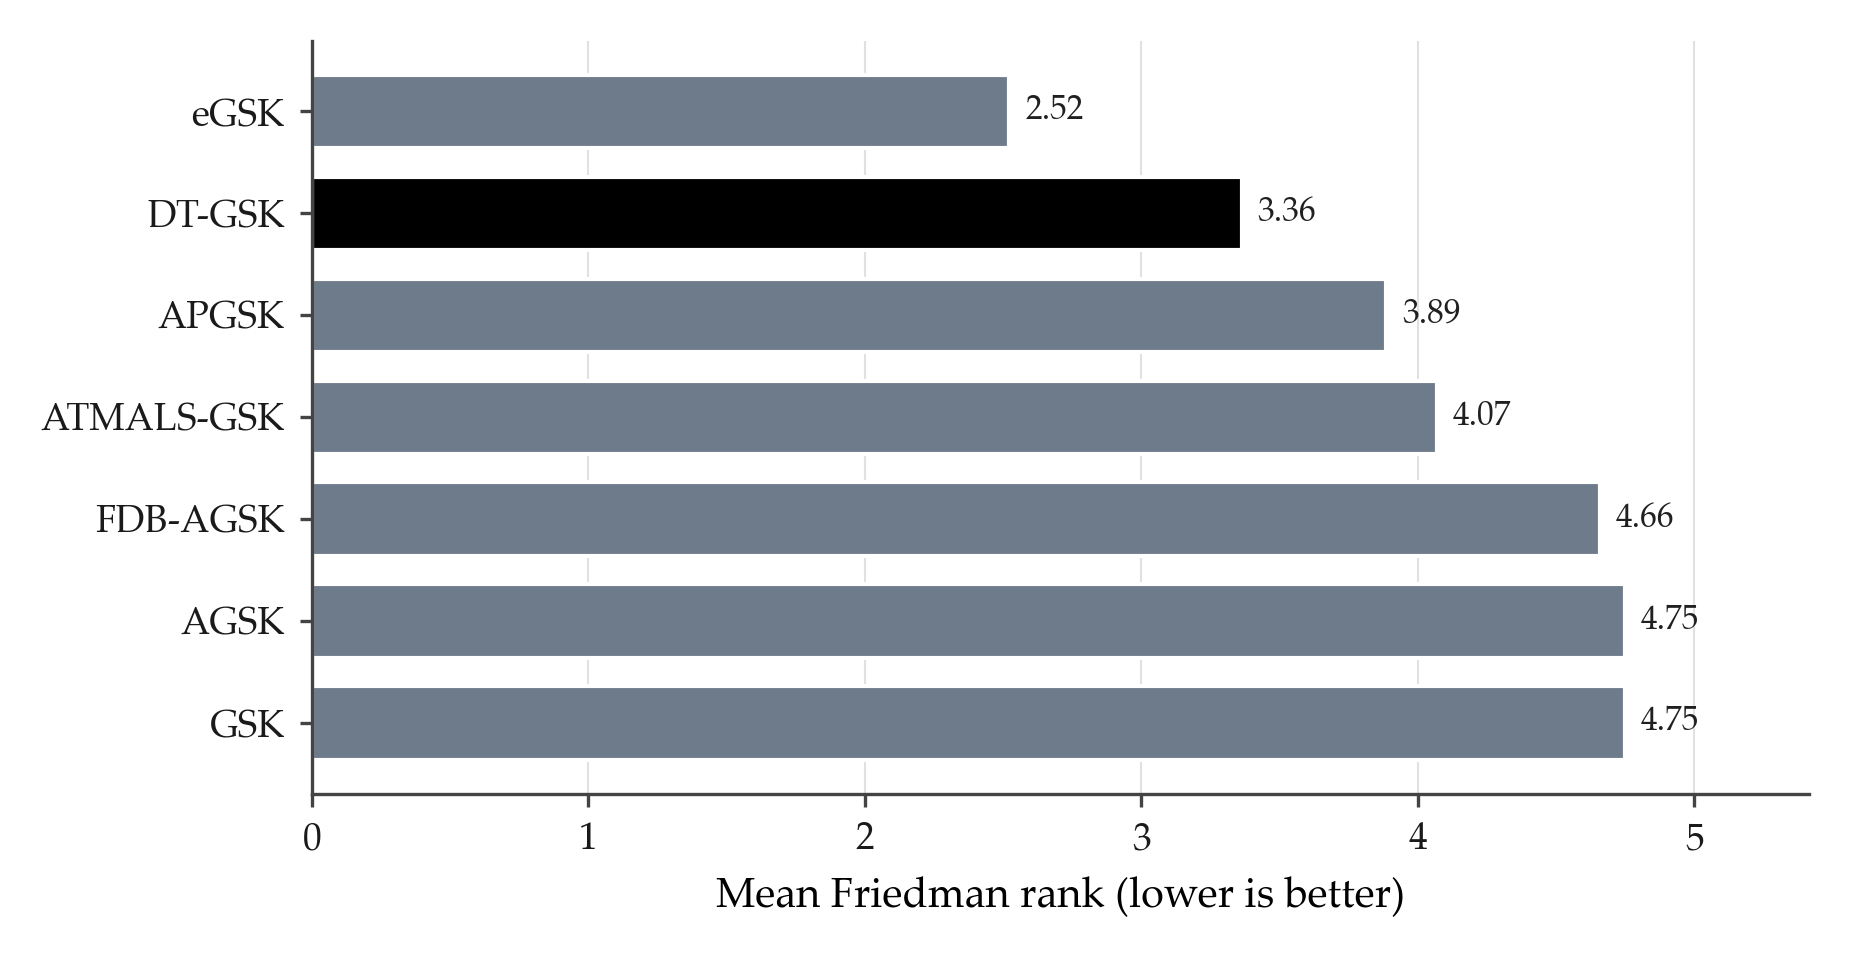
\includegraphics[width=0.70\textwidth]{figures/ranks/cec2011_ranks.png}
\caption{@@FIGCAP!fig:cec2011-ranks@@ Friedman mean ranks over the 22 CEC2011 real-world problems
(25 runs each, raw best-fitness basis), sorted best-first; \dtgsk{}
highlighted. Lower is better. 
Within this panel \dtgsk{}'s across-problem Wilcoxon vs.\ \egsk{} is
a significant loss (Holm $p = 4.2 \times 10^{-2}$).}\label{fig:cec2011-ranks}

\end{figure}


\subsection{@@SECNUM!sec:exp:cec2013!4.4.@@ Results on the CEC2013 Second Comparison Suite}\label{sec:exp:cec2013}


CEC2013 is reported as a second comparison suite --- for breadth of
comparison under the identical protocol --- and carries no
independence claim of any kind. The per-function five-statistic
tables and the Wilcoxon summaries are in the Supplementary Materials,
Section~S2; the panel-level numbers quoted here are re-derivable from
the released analysis bundle.


Within the GSK-family panel, \dtgsk{} attains the best overall
Friedman mean rank on CEC2013 (2.80, unweighted mean of the three
per-dimension mean ranks, the same descriptive convention as
Table~@@REF!tab:friedman-cec2017@@; \egsk{} is second at 3.41).
Table~@@REF!tab:friedman-cec2013@@ reports the full per-dimension panel.


\begin{table}[H]
\caption{@@TABLECAP!tab:friedman-cec2013@@ Friedman mean ranks (lower is better) of the seven-algorithm
GSK-family panel on the CEC2013 second comparison suite per dimension
(28 per-function mean errors as blocks, 51 runs each) plus the
unweighted across-dimension mean (``Overall'', a descriptive
aggregate); the Friedman + Iman--Davenport omnibus is significant at
every dimension ($p \leq 1.1 \times 10^{-3}$). Best rank per column in
bold. CEC2013 is reported for breadth of comparison and carries no
independence claim. }\label{tab:friedman-cec2013}
\zebra
\begin{tabular}{lcccc}
\toprule
\textbf{Algorithm} & \textbf{D10} & \textbf{D30} & \textbf{D50} & \textbf{Overall} \\
\midrule
GSK & 5.88 & 4.98 & 5.16 & 5.34 \\
\agsk{} & 3.80 & 4.48 & 4.52 & 4.27 \\
\apgsk{} & 3.88 & 4.63 & 4.79 & 4.43 \\
\fdbagsk{} & 3.95 & 4.13 & 4.27 & 4.11 \\
\atmals{} & 4.21 & 3.34 & 3.38 & 3.64 \\
\egsk{} & 3.88 & \textbf{3.07} & 3.29 & 3.41 \\
\dtgsk{} & \textbf{2.41} & 3.38 & \textbf{2.61} & \textbf{2.80} \\
\bottomrule
\end{tabular}

\end{table}

The per-dimension picture is first/third/first: at $D = 10$,
\dtgsk{} leads with mean rank 2.41 (omnibus
$p = 5.3 \times 10^{-8}$); at $D = 30$ it places \emph{third} (3.38)
behind \egsk{} (3.07) and \atmals{} (3.34) (omnibus
$p = 1.1 \times 10^{-3}$); at $D = 50$ it leads again with 2.61
(omnibus $p = 2.9 \times 10^{-6}$).

The $D = 30$ third place is disclosed as this suite's counterpart of
the CEC2017 mid-dimension weakness; the across-function
Holm-corrected Wilcoxon tests at $D = 30$ against both \egsk{} and
\atmals{} show no significant difference ($p_{\mathrm{Holm}} = 0.748$
each), so the deficit is ordinal, not statistically separable.

Against the original GSK, \dtgsk{} records Holm-significant wins at
all three dimensions
($p_{\mathrm{Holm}} = 1.9 \times 10^{-4}$, $3.1 \times 10^{-2}$, and
$2.7 \times 10^{-3}$ at $D = 10/30/50$; win/tie/loss 24--2--2,
21--2--5, and 24--2--2; $R^{+}/R^{-} = 340/11$, $286/65$, and
$314/37$).

The dimension profile of these outcomes mirrors the primary suite:
the mid-dimension tier is where the improved family variants ---
\egsk{} and \atmals{} in particular --- are hardest to separate,
while the low- and upper-dimension tiers favor \dtgsk{} within the
panel.

Because these results come from the same protocol and pairing as the
primary suite, they are read as breadth of comparison within the GSK
family panel, not as evidence of generalization beyond the suites
tested.



\subsection{@@SECNUM!sec:exp:cec2020!4.5.@@ Results on the CEC2020 Pre-Registered Confirmatory Suite}\label{sec:exp:cec2020}


CEC2020 is the one suite in this study whose entire analysis --- the
hypotheses, the analysis families, the tie rules, and the three candidate
outcome sentences --- was committed to the repository before any CEC2020
result existed, at the signing commit 5c9bfae82 of the registered
analysis-plan addendum. The complete registered battery, its robustness
checks, and the mid-campaign inspection ledger are reported in
Supplementary Section~S8, and the outcome sentence below is the
pre-committed wording-bank variant selected by the data, not re-drafted
after the fact.

The protocol is the registered one of Table~@@REF!tab:protocol@@: 10
functions at $D \in \{5, 10, 15, 20\}$, with F6 and F7 undefined at
$D = 5$ (38 scored cells), 30 runs per cell, a MaxFES that rises from
$5 \times 10^{4}$ at $D = 5$ to $10^{7}$ at $D = 20$, and the error
basis with the $10^{-8}$ floor.


On AGSK's strongest suite --- the CEC2020 competition in which it was
the runner-up~@@CITE!apgsk2021@@ --- \dtgsk{} places fourth; the family
panel corroborates AGSK's published strength in this regime, consistent
with the tiering thesis: every dimension-gated \dtgsk{} subsystem is
inactive at $D \leq 20$.

The descriptive across-dimension aggregate (the unweighted mean of the
four per-dimension Friedman mean ranks; no test is attached, the $D = 5$
task set is reduced to 8 functions, and MaxFES changes by dimension, so
the aggregate mixes budget regimes) is 4.11 for \dtgsk{}, fourth of
seven; \agsk{} is best at 2.09, \fdbagsk{} second at 2.31, and \apgsk{}
third at 3.09.

Per dimension, the Friedman--Iman--Davenport omnibus separates the panel
at every dimension ($p \leq 6.1 \times 10^{-5}$), with the registered
seeded permutation check agreeing at each; the mean ranks place \dtgsk{}
at 4.25 (fourth) at $D = 5$, 4.10 (fourth) at $D = 10$, 3.50 (tied-third
with \apgsk{}) at $D = 15$, and 4.60 (fifth) at $D = 20$, while \agsk{}
holds the best mean rank at $D \in \{10, 15, 20\}$ (1.90, 2.10, 1.60)
and \apgsk{} at $D = 5$ (2.38).
Table~@@REF!tab:cec2020-ranks@@ reports the complete panel.


\begin{table}[H]
\caption{@@TABLECAP!tab:cec2020-ranks@@ CEC2020 final panel results: tie-corrected Friedman mean ranks per
dimension (lower is better; 30 runs per cell, error basis with the $10^{-8}$
floor) and the descriptive across-dimension aggregate. No test is attached to
the aggregate: the $D=5$ task set is reduced to 8 functions (F6 and F7 are
undefined there), and MaxFES changes with dimension, so the aggregate mixes
budget regimes. The omnibus rows give the tie-corrected Friedman statistic,
the Iman--Davenport $p$, and the registered seeded permutation $p$
($B = 10^{5}$). Per-dimension ranks are exact at three decimals ($N$ = 8 or
10); the aggregate, their unweighted mean, is printed at four. Per-function
detail, run-level tests, and effect sizes are in Supplementary
Section~S8.}\label{tab:cec2020-ranks}
\setlength{\tabcolsep}{5pt}
\begin{tabular}{lccccc}
\toprule
\textbf{Algorithm} & $\bm{D=5}$ & $\bm{D=10}$ & $\bm{D=15}$ & $\bm{D=20}$ & \textbf{Aggregate} \\
\midrule
\agsk{} & 2.750 & \bestval{1.900} & \bestval{2.100} & \bestval{1.600} & \bestval{2.0875} \\
\fdbagsk{} & 2.750 & 2.200 & 2.300 & 2.000 & 2.3125 \\
\apgsk{} & \bestval{2.375} & 3.000 & 3.500 & 3.500 & 3.0938 \\
\dtgsk{} & 4.250 & 4.100 & 3.500 & 4.600 & 4.1125 \\
\egsk{} & 4.875 & 5.400 & 5.500 & 6.000 & 5.4437 \\
GSK & 5.625 & 6.200 & 5.500 & 4.500 & 5.4562 \\
\atmals{} & 5.375 & 5.200 & 5.600 & 5.800 & 5.4938 \\
\midrule
Functions ($N$) & 8 & 10 & 10 & 10 & --- \\
Friedman $\chi^{2}$ (tie-corr.) & 23.22 & 40.24 & 37.66 & 42.52 & --- \\
Iman--Davenport $p$ & $6.1\times10^{-5}$ & $1.8\times10^{-11}$ & $4.3\times10^{-10}$ & $7.2\times10^{-13}$ & --- \\
Permutation $p$ & $7.0\times10^{-5}$ & $1.0\times10^{-5}$ & $1.0\times10^{-5}$ & $1.0\times10^{-5}$ & --- \\
\bottomrule
\end{tabular}





\end{table}
In the registered across-function pairwise layer, \dtgsk{} is
Holm-separated in five of the twenty-four comparator--dimension cells:
three favorable --- against \atmals{} and \egsk{} at $D = 15$, and
against \egsk{} at $D = 20$ --- and two unfavorable --- against \agsk{}
and \fdbagsk{} at $D = 20$. In the remaining nineteen cells, including
every comparison at $D = 5$ and $D = 10$, no separation is demonstrated.

This fourth place is the boundary finding that the registered directional
expectation predicted in advance --- \agsk{} and \apgsk{} favored on
their home regime, every dimension-gated \dtgsk{} subsystem structurally
off at $D \leq 20$ --- and it is reported as such, not as a result that
``does not count''; no CEC2020 sentence in this paper claims superiority
over \agsk{} or \fdbagsk{} at any dimension.

One conflict adjacency accompanies every interpretation of this suite,
here as in the back matter: \agsk{} was the runner-up of the CEC2020
competition~@@CITE!apgsk2021@@, and its paper is a co-author's.



\subsection{@@SECNUM!sec:exp:cec2013lsgo!4.6.@@ Results on the CEC2013LSGO Large-Scale Suite}\label{sec:exp:cec2013lsgo}


The CEC2013LSGO analysis in this paper is family-internal: it ranks the
seven GSK-family variants against one another under a common protocol.
Dedicated large-scale optimizers --- for example
SHADE-ILS~@@CITE!molina2018shadeils@@ and MOS~@@CITE!latorre2013mos@@ ---
report substantially stronger published results on this suite than any
GSK-family member, and no competitiveness with such specialists is
claimed here; cross-paradigm comparison is outside this paper's scope.

The suite's evidential tier is disclosed rather than implied: the
descriptive layer (mean ranks, omnibus, win/tie/loss) was inspected
informally before the analysis addendum was signed and therefore carries
no confirmatory weight, whereas the run-level paired layer had never
been computed before registration and is confirmatory-with-disclosure;
both are reported in full, with this provenance, in Supplementary
Section~S7.


Descriptively, \dtgsk{} and \agsk{} share the best family mean rank
(tied-first, 3.13 each, over the 15 function blocks); no member except
\egsk{} (worse, at 5.47) is separable by the omnibus procedure at the
Nemenyi critical distance of 2.33, and \dtgsk{} is last on F7 and F15.
Table~@@REF!tab:lsgo-ranks@@ reports the final family panel.


\begin{table}[H]
\caption{@@TABLECAP!tab:lsgo-ranks@@ CEC2013LSGO final family panel: tie-corrected Friedman mean ranks
over the 15 function blocks (raw best-objective basis, 25 runs per cell;
lower is better) with the across-function Wilcoxon layer against \dtgsk{}
(win--tie--loss on per-function means, tie band $10^{-8}$; exact
two-sided sign-flip $p$; Holm-adjusted over the six comparators). The
descriptive columns carry no confirmatory weight (inspected before
registration); the pairwise columns are the registered
supporting-with-disclosure layer, and no comparator separates from
\dtgsk{}. An exact rank tie is reported as tied-first, never absorbed.
Omnibus: Friedman $\chi^{2} = 15.31$, Iman--Davenport $p = 0.014$;
Nemenyi critical distance $2.33$ ($k = 7$, $N = 15$). Run-level tests and
effect sizes are in Supplementary Section~S7.}\label{tab:lsgo-ranks}
\setlength{\tabcolsep}{5pt}
\begin{tabular}{lccccc}
\toprule
\textbf{Algorithm} & \textbf{Mean rank} & \textbf{Ordinal} &
\textbf{\dtgsk{} W--T--L} & \textbf{Exact} $\bm{p}$ & \textbf{Holm} $\bm{p}$ \\
\midrule
\dtgsk{} & \bestval{3.133} & 1 (tied-first) & --- & --- & --- \\
\agsk{} & \bestval{3.133} & 1 (tied-first) & 9--0--6 & 0.8469 & 1.0000 \\
\atmals{} & 3.533 & 3 & 8--0--7 & 0.1688 & 0.5065 \\
GSK & 3.867 & 4 & 8--0--7 & 0.7615 & 1.0000 \\
\fdbagsk{} & 3.933 & 5 & 11--0--4 & 0.0833 & 0.3330 \\
\apgsk{} & 4.933 & 6 & 11--0--4 & 0.0554 & 0.2875 \\
\egsk{} & 5.467 & 7 & 11--0--4 & 0.0479 & 0.2875 \\
\bottomrule
\end{tabular}




\end{table}
The registered paired layers resolve the standing: across functions, no
comparator separates from \dtgsk{} after Holm correction, and in
particular the paired tests do not separate \dtgsk{} from \agsk{} (exact
$p = 0.847$, Holm-adjusted $1.0$) --- the registered ceiling wording,
tied-first descriptive rank with no paired separation, applies verbatim.

At run level the picture is regular in both directions, and both are
stated: \dtgsk{} is Holm-significantly better than every one of the six
family members on F4 and F8, and Holm-significantly worse than every one
of them on F7 and F15.

The effect layer bars any superiority reading against \atmals{}: the
mean run-level effect across the 15 functions marginally favors that
comparator (mean Cliff's delta $-0.0025$ against \dtgsk{}), so the
effect layer supports no superiority claim over \atmals{} on this suite.

The one \dtgsk{}-specific configuration addition on this suite --- the
two linkage-block-size entries for $D = 905$ and $D = 1000$ described in
Section~@@REF!sec:exp:settings@@ --- is disclosed, with its rule,
rationale, and timing, in Supplementary Section~S7.



\subsection{@@SECNUM!sec:exp:convergence!4.7.@@ Convergence Analysis}\label{sec:exp:convergence}


Figures~@@REF!fig:conv-cec2017-d30@@ and~@@REF!fig:conv-cec2017-d100@@
show family-overlay convergence curves on CEC2017 at the two featured
dimensions. The function selection was prespecified and frozen
before rendering, stratified over function category, difficulty tercile, and
\dtgsk{} standing, and it deliberately includes an unfavorable case.
At $D = 30$ the selected panel comprises F3 (unimodal, easy/strong),
F10 (simple multimodal, hard/comparable), F12 (hybrid, hard/comparable),
and F26 (composition, hard/weak --- the mandated unfavorable case).
At $D = 100$ it comprises F1 (unimodal, easy/strong),
F5 (simple multimodal, easy/strong), F12 (hybrid, hard/comparable),
and F26 (composition, hard/comparable).

Every curve is the per-checkpoint \emph{mean} error across all 51
runs of that algorithm --- the identical aggregation basis for all
seven curves in every panel, with no smoothing and no
interpolation --- on a log-error axis whose display-only floor of
$10^{-14}$ marks exact zeros and never enters any statistic. The
complete function $\times$ dimension convergence sets for CEC2017,
CEC2011 and CEC2013 are in the Supplementary Materials, Section~S3.


The unfavorable case is discussed rather than skipped. On F26 at
$D = 30$, \dtgsk{}'s final mean error ($1.16 \times 10^{3}$) is
higher than five of the six comparators; only \atmals{}
($1.32 \times 10^{3}$) ends higher. Its best run
($9.85 \times 10^{2}$) never reaches the low attractor that every
comparator's best run reaches ($2.00$--$3.00 \times 10^{2}$). At the
same time its standard deviation ($7.5 \times 10^{1}$) is the
smallest in the panel, the next smallest being GSK's
$2.7 \times 10^{2}$.

The measured pattern at this cell is thus consistent mid-level
convergence without basin escapes, on a composition function at the
dimension where the structure-memory subsystems are inactive
(Section~@@REF!sec:algorithm@@); per-component attribution is not
claimed.

At $D = 100$ the same function is a comparable case: \dtgsk{}'s
final mean error ($4.09 \times 10^{3}$) sits below four comparators
(\atmals{} $5.55 \times 10^{3}$; \fdbagsk{} $1.03 \times 10^{4}$;
\agsk{} $1.10 \times 10^{4}$; \apgsk{} $1.22 \times 10^{4}$) and
above GSK ($3.69 \times 10^{3}$) and \egsk{}
($3.05 \times 10^{3}$).


\begin{figure}[H]
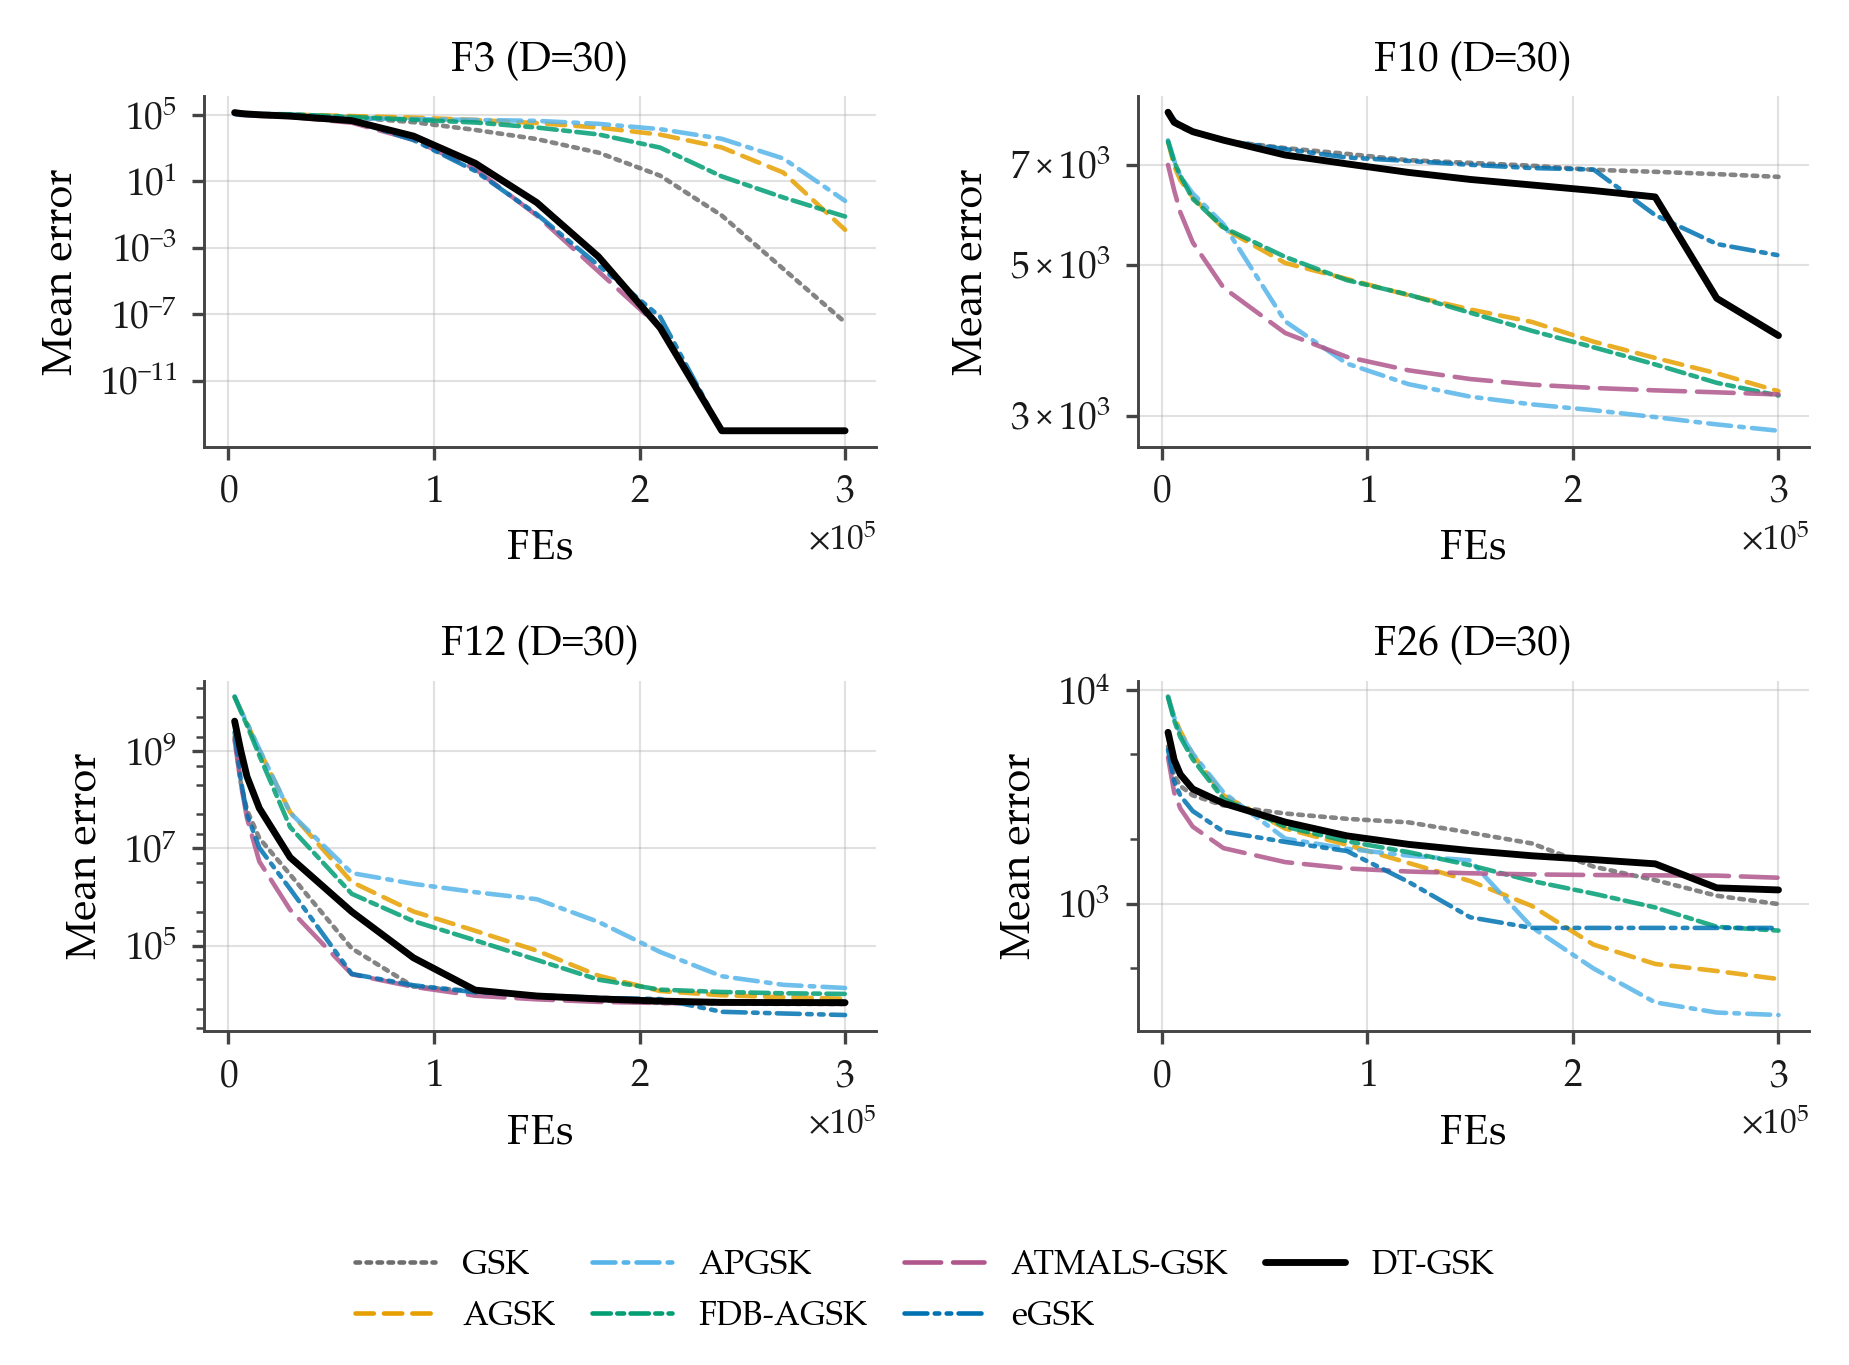
\includegraphics[width=0.92\textwidth]{figures/convergence/main_cec2017_D30.png}
\caption{@@FIGCAP!fig:conv-cec2017-d30@@ Family-overlay convergence on CEC2017 at $D = 30$ for the
four functions selected by a fixed, prespecified rule and frozen before rendering:
F3 (unimodal; easy/strong), F10 (simple multimodal;
hard/comparable), F12 (hybrid; hard/comparable), F26 (composition;
hard/weak --- the mandated unfavorable case). Each panel overlays all
7 panel algorithms; every curve is the per-checkpoint mean error
across 51 runs (identical basis; no smoothing); log-error $y$-axis
with a display-only floor of $10^{-14}$ for exact zeros (never enters
any statistic); one shared legend. $D = 30$ is \dtgsk{}'s known-weak
tier: rank \#2 behind \egsk{}. 
APGSK checkpoint evidence at $D = 30$ carries the per-run availability
qualification of
Section~@@REF!sec:exp:settings@@.}\label{fig:conv-cec2017-d30}

\end{figure}

\begin{figure}[H]
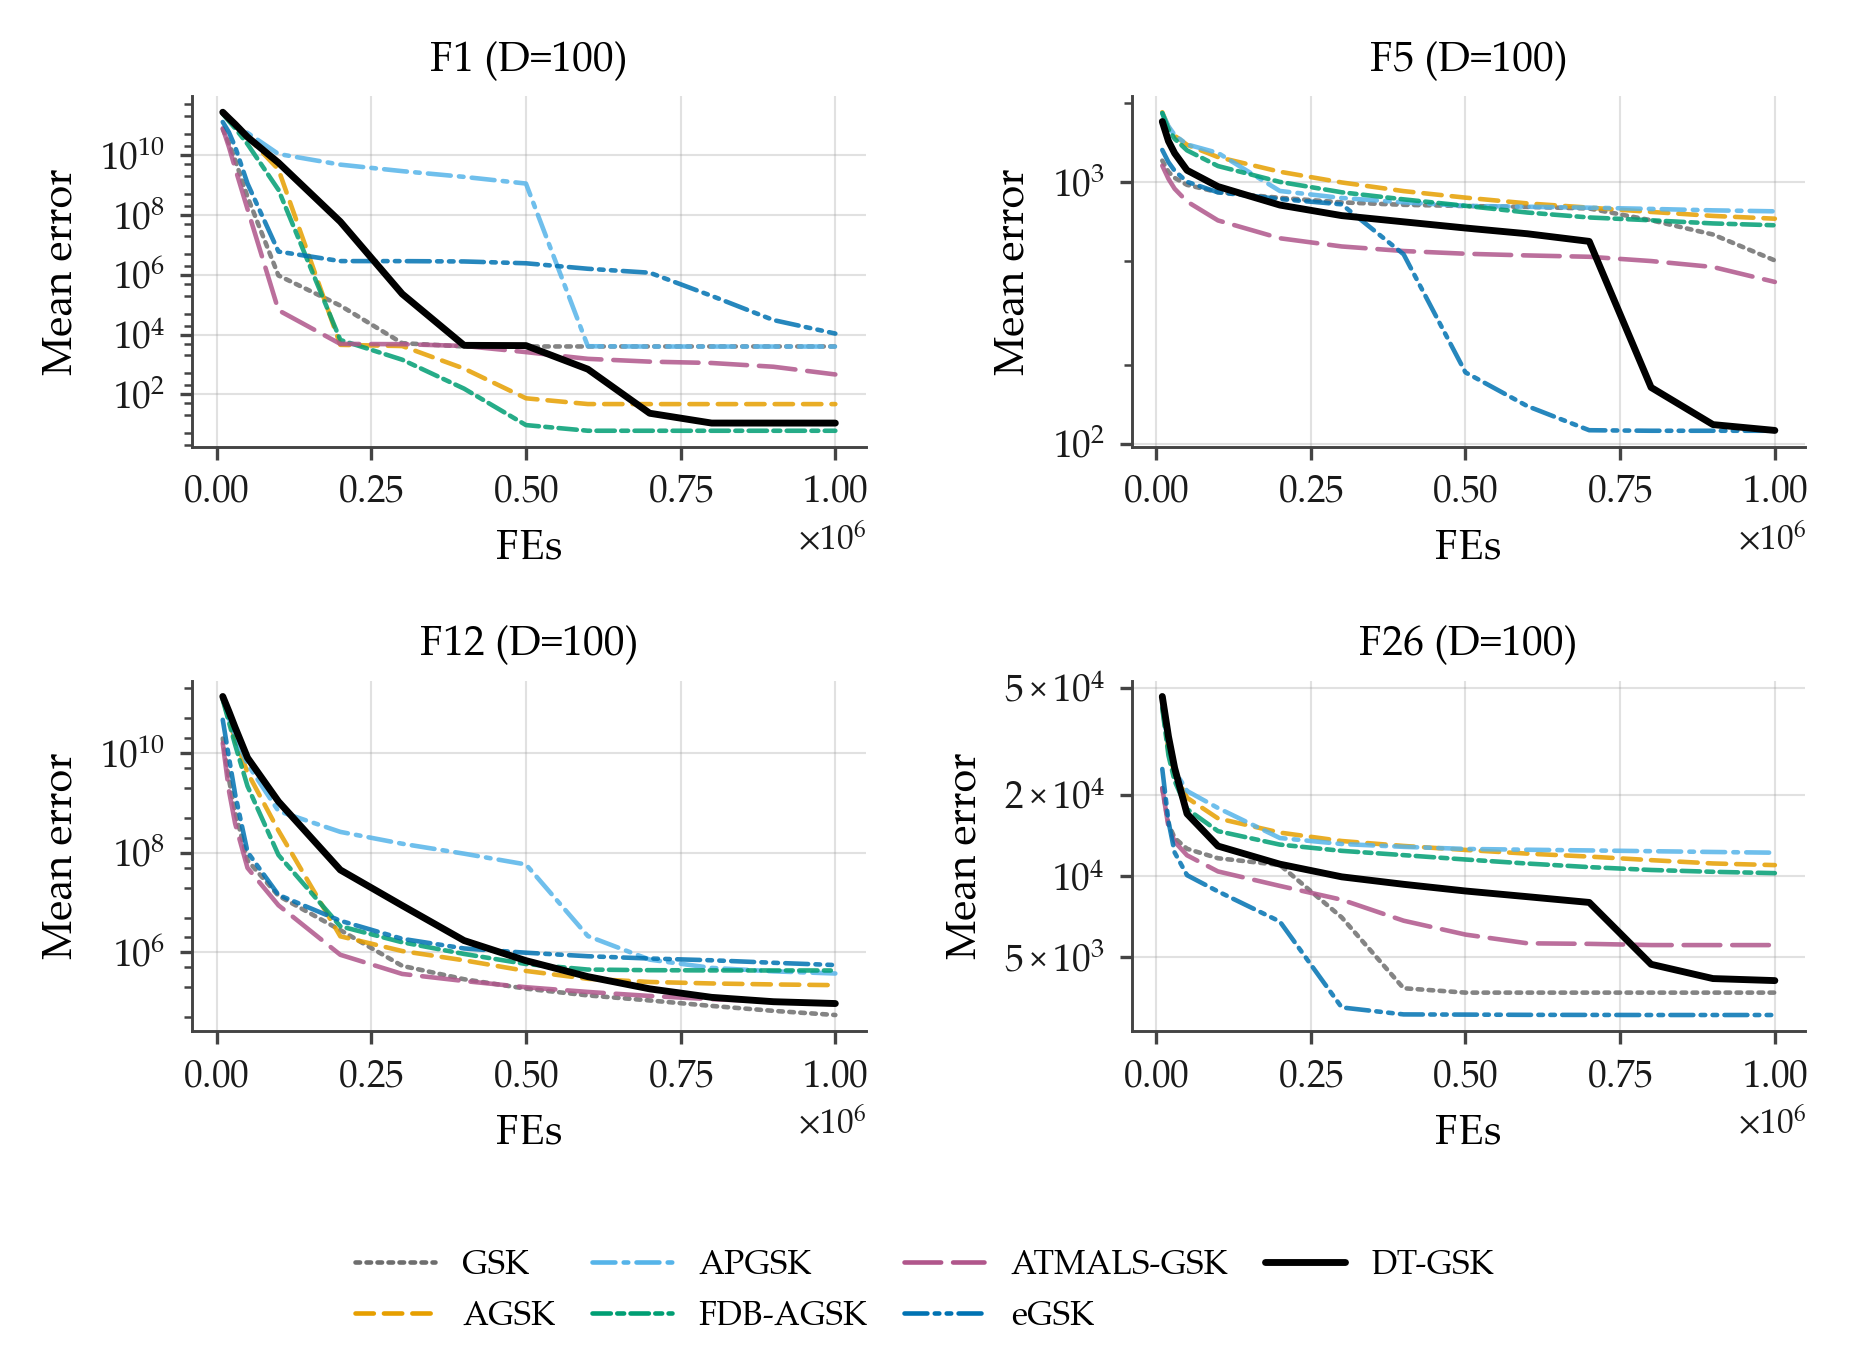
\includegraphics[width=0.92\textwidth]{figures/convergence/main_cec2017_D100.png}
\caption{@@FIGCAP!fig:conv-cec2017-d100@@ Family-overlay convergence on CEC2017 at $D = 100$ (tier
where the structure-memory and polish subsystems are active) for the
four prespecified functions: F1 (unimodal; easy/strong), F5 (simple
multimodal; easy/strong), F12 (hybrid; hard/comparable), F26
(composition; hard/comparable). Per-checkpoint mean error across 51
runs per algorithm, 7-curve overlay, log-error $y$-axis (display
floor $10^{-14}$), one shared legend. }\label{fig:conv-cec2017-d100}

\end{figure}


\subsection{@@SECNUM!sec:exp:runtime!4.8.@@ Runtime and Complexity in Practice}\label{sec:exp:runtime}


Table~@@REF!tab:runtime@@ reports \dtgsk{}'s measured per-run wall-clock time on
CEC2017 (mean $\pm$ SD over the 1{,}479 runs per dimension cell, i.e., 29
functions $\times$ 51 runs), collected in a single environment: the 51-run
post-fix campaign with the interaction graph's compiled kernels active. The
comparator timings were collected in a separate measurement session, so we do
not tabulate a cross-algorithm wall-clock comparison and make no
runtime-superiority claim; the figures characterize \dtgsk{}'s own cost.


\dtgsk{}'s per-run time scales with dimension, from 4.93~s at $D = 10$ to
41.59~s at $D = 100$ --- the bookkeeping cost of its scaffold and
structure-memory subsystems on top of the unchanged GSK vector-update operator. These are
measured costs at matched evaluation budgets: the overhead is bookkeeping, not
extra objective evaluations (Section~@@REF!sec:algorithm@@), and it grounds the
overhead limitation restated in the conclusions. These measurements are the
empirical counterpart of the per-tier asymptotic cost model in
Section~@@REF!sec:alg:complexity@@, so cost is reported both analytically and in
wall-clock terms. The isolated compute cost of
the interaction-structure memory is quantified in the Supplementary Materials
(Section~S6.5; the measurement provenance for those figures is recorded in
Section~S6.7). On the other suites \dtgsk{}'s mean per-run time is
4.45--34.26~s across CEC2013 $D \in \{10, 30, 50\}$ and 80.64~s on CEC2011
(native dimensions). No comparator wall-clock is reported anywhere in this
paper: comparator timings were collected in a separate measurement session, so
placing them beside these figures would confound implementation and hardware
differences with algorithmic cost. The runtime evidence therefore characterizes
\dtgsk{}'s own cost and its scaling with dimension, and supports no
cross-algorithm efficiency claim.


\begin{table}[H]
\caption{@@TABLECAP!tab:runtime@@ Measured per-run wall-clock time of \dtgsk{} on CEC2017 (seconds; mean
$\pm$ SD over 1{,}479 runs per cell $=$ 29 functions $\times$ 51 runs), collected
in a single environment: the 51-run post-fix campaign with the interaction
graph's compiled kernels active (an earlier release had silently executed the
bit-for-bit-equivalent \textsc{NumPy} reference path, inflating wall-clock only).
No comparator wall-clock is tabulated, so no cross-algorithm runtime comparison
is made. The isolated
interaction-structure-memory overhead is reported in the Supplementary Materials,
Section~S6.5.}\label{tab:runtime}
\zebra
\begin{tabular}{lc}
\toprule
\textbf{CEC2017 dimension} & \textbf{\dtgsk{} per-run wall-clock (s)} \\
\midrule
$D = 10$ & $4.93 \pm 0.83$ \\
$D = 30$ & $13.04 \pm 2.69$ \\
$D = 50$ & $23.30 \pm 5.23$ \\
$D = 100$ & $41.59 \pm 13.95$ \\
\bottomrule
\end{tabular}

\end{table}


\subsection{@@SECNUM!sec:exp:discussion!4.9.@@ Discussion}\label{sec:exp:discussion}


\paragraph{Alternative explanations for the standing.}
Three deserve explicit statement. First, the strongest measured component
effect belongs to the deterministic endgame \emph{as a whole}, and the polish
isolation removes that entire compass phase rather than the learned basis
alone, so the advantage may rest on classical direct search rather than on
anything learned during the run. Second, \dtgsk{} begins from
$NP = 5D$ against the comparators' $NP = 100$ --- a five-fold difference at
$D = 100$ --- which is a design choice inherited from the family's
reference-implementation configuration rather than a controlled variable. Third, CEC2017 is
development-exposed; CEC2011 and CEC2013 corroborate, but neither is
independent of configuration selection --- the single configuration was fixed on
CEC2017 before either suite was seen, so they were not consulted for selection yet
cannot be read as fully independent holdouts. None of the three is excluded by the
evidence reported here, and each bounds how far the panel standing should be
read as attributable to the tiered design itself. A fourth bound is
evidential role rather than alternative explanation: CEC2020 is the one
suite whose analysis plan, hypotheses and outcome wording were committed
before any of its data existed (the registered addendum's signing commit
precedes the first CEC2020 result; Section~@@REF!sec:exp:cec2020@@ and
Supplementary Section~S8), whereas CEC2013LSGO's descriptive layer was
inspected before registration and therefore carries no confirmatory
weight (Supplementary Section~S7).


\paragraph{By function class.}
The class-wise reading of
Section~@@REF!sec:exp:cec2017:desc@@ is that \dtgsk{}'s standing
within the panel is strongest on the hybrid class at $D \geq 30$
(best or equal-best class mean rank at all three dimensions) and on
the simple multimodal class away from $D = 30$. Its weakest cell is the
composition class at $D = 10$, where the class mean rank is 3.70, behind
three comparators.

This distribution is consistent with the design intent of
block-structured recombination on partially separable (hybrid)
landscapes. The inherited fixed-size (non-contiguous) block variant is
already active at $D = 30$, where the memory-driven channel is not, and the
ISM-supplied linkage blocks join it at $D \geq 50$. This is stated as
plausibility, not as a measured component contribution: the
mechanisms of
Section~@@REF!sec:algorithm@@ are proposed
and fully specified, and per-component causal attribution is
deliberately not claimed in this paper.


\paragraph{By dimension.}
The rank-versus-dimension trend (2.88,
2.50, 2.21, 2.34; plotted in the Supplementary Materials) is interpreted as
within-panel scalability behavior over the four CEC2017 tiers only.
\dtgsk{}'s relative standing
improves from $D = 10$ to $D = 50$ and remains first at $D = 100$.
The trend is not monotone, however: $D = 30$ is an ordinal dip to
second behind \egsk{}, and $D = 100$ is slightly worse than $D = 50$.

The upper-tier ($D \geq 50$) behavior (Figures~@@REF!fig:conv-cec2017-d100@@
and~@@REF!fig:cd-cec2017@@; Table~@@REF!tab:friedman-cec2017@@) arises under
the frozen configuration, in which the interaction-structure memory
and several subsystems --- the eigenframe polish and the raised population
floor --- co-activate at $D \geq 50$.
This reading associates the upper-tier behavior with the bundled
tier configuration rather than with any isolated component. A direct
isolation of the interaction-structure memory (Supplementary Materials
Section~S6.5) finds no significant standalone benefit at its active
tiers, at a tier-dependent compute overhead; per-component attribution to
the memory is therefore not claimed here (Section~@@REF!sec:conclusions@@).
Conversely, at $D \leq 30$ \dtgsk{} runs essentially the
adaptive scaffold, so low-dimension behavior --- including the
$D = 30$ second place and the composition-class weakness at
$D = 10$ --- reflects this structural gating rather than the tier-gated
mechanisms.


\paragraph{By aggregate counts.}
Across the 24 Holm-corrected CEC2017 cells, \dtgsk{} records 17
significant wins, 7 with no significant difference, and no significant loss
(Table~@@REF!tab:wilcoxon-holm@@). That is a descriptive across-dimension tally:
the four within-dimension Holm families are not pooled. The
no-difference cells concentrate against
\egsk{}, whose head-to-head win/tie/loss records favor it at
$D \geq 30$ (11--2--16, 13--0--16, 12--0--17) even where \dtgsk{}
holds the better Friedman rank. The two are never
Nemenyi-separable on this suite.

On CEC2011, the aggregate is two significant wins, three with no
significant difference, and one significant loss --- the loss to \egsk{}
($p_{\mathrm{Holm}} = 4.2 \times 10^{-2}$) --- so the real-world
suite corroborates competitive placement (second of seven) within the
family panel, not first place.

On CEC2013, the overall first place (2.80) coexists with a $D = 30$
third place (3.38) behind \egsk{} and \atmals{}.

On CEC2020, the across-function tally is three Holm-significant wins,
two Holm-significant losses, and nineteen cells with no separation
demonstrated, over four independent within-dimension Holm families
(Section~@@REF!sec:exp:cec2020@@).

On CEC2013LSGO, the across-function paired layer separates no comparator
from \dtgsk{}, and the run-level regularity --- better than all six on
F4 and F8, worse than all six on F7 and F15 --- is stated in both
directions (Section~@@REF!sec:exp:cec2013lsgo@@).

Taken together, the evidence supports one calibrated statement:
within the GSK-family panel and under the frozen budget-fair
protocol, \dtgsk{} is first on two, tied-first on one, second on one,
and fourth on one of the five suites' descriptive family-rank
aggregates --- first on CEC2017 (2.48) and CEC2013 (2.80), tied-first
with \agsk{} on CEC2013LSGO (3.13 each, with no paired separation),
second on CEC2011 (3.36), and fourth on CEC2020 (4.11), the
pre-registered confirmatory suite, where the wording-bank outcome
sentence of Section~@@REF!sec:exp:cec2020@@ applies. No statistic pools
suites, so this count of independent per-suite descriptive standings is
the only cross-suite statement made. \egsk{} holds the better ordinal
rank at the mid-dimension tier, at $D = 30$ on both CEC2017 and CEC2013, where
the paired tests do not establish a separation, and a Holm-significant
advantage on CEC2011.

These rank statements carry the robustness qualification of
Section~@@REF!sec:exp:stats@@: \dtgsk{}'s own ordinals are stable
under the median re-ranking variant and the variant excluding the disputed cells, but
several comparator orderings are not.

Consistent with no-free-lunch considerations, none of these findings
is offered as evidence of field-wide superiority: every comparative
claim in this paper is bounded to the cited suites, budgets, and the
seven-algorithm GSK-family panel~@@CITE!wolpert1997nfl@@.

















\section{@@SECNUM!sec:conclusions!5.@@ Conclusions}\label{sec:conclusions}


This paper introduced \dtgsk{}, a GSK-family algorithm that retains the
gaining-sharing vector-update equations and layers an adaptive control-and-budget
scaffold, a deterministic final polish, and a controlled family evaluation on that
core, with an interaction-structure memory as a supporting mechanism. 
That memory is a decaying, confidence- and evidence-gated
coordinate-pair graph learned from the moves the run has already
accepted. It is active at $D \geq 50$ and consumed
twice --- as linkage blocks for the block crossover, and as the eigenbasis of
the one-shot, RNG-free final polish. An ISM-block subspace local search is
implemented but not enabled in the frozen configuration. 
A dimension-tiered scaffold (ACE with ARGP pruning, the tier-floored
NLPSR schedule, the hard-capped BSE, and a deep-stall restart that
preserves the global best) carries the tiers where the memory is
inactive, and one hash-frozen configuration serves every dimension of
the four bound-constrained suites, with a single disclosed large-scale
exception
(Supplementary Section~S7). 

The empirical findings are panel-scoped and dimension-resolved --- the
study characterizes the algorithm's standing tier by tier rather than
claiming uniform dominance --- and the unfavorable cells are stated with
the favorable ones. Within the seven-algorithm GSK-family panel
on CEC2017, \dtgsk{} attains the best overall Friedman mean rank ---
2.48, the unweighted mean of the four per-dimension ranks, with
\egsk{} second at 2.96 --- placing first at $D = 10/50/100$ (2.88,
2.21, 2.34) and second at $D = 30$ (2.50) behind \egsk{}
(2.29). 
Across the 24 Holm-corrected pairwise cells it records 17 significant
wins, 7 with no significant difference, and no significant loss --- a
descriptive tally over four independent within-dimension Holm families
(size 6 each), not a single result controlled family-wise across
dimensions. 
At the same time, its head-to-head records against \egsk{} at
$D \geq 30$ are losing ones (11--2--16, 13--0--16, 12--0--17), and the
two algorithms are never Nemenyi-separable on this suite (all four rank
gaps lie inside the critical difference of
1.67). 
On CEC2011, \dtgsk{} places second of seven (3.36; \egsk{} first at
2.52), and its across-problem Wilcoxon against \egsk{} is a
Holm-significant loss
($p_{\mathrm{Holm}} = 4.2 \times 10^{-2}$). 
On the CEC2013 second comparison suite, the overall descriptive
aggregate is again the panel's best (2.80), with a per-dimension
profile of first/third/first --- third at $D = 30$ behind \egsk{} and
\atmals{}. 
On AGSK's strongest suite --- the CEC2020 competition in which it was
the runner-up~@@CITE!apgsk2021@@ --- \dtgsk{} places fourth; the family
panel corroborates AGSK's published strength in this regime, consistent
with the tiering thesis: every dimension-gated \dtgsk{} subsystem is
inactive at $D \leq 20$. That suite is the pre-registered confirmatory
leg --- its analysis and outcome wording were committed before any of
its data existed --- and \dtgsk{} is Holm-separated in only five of its
twenty-four pairwise cells, three favorable and two
unfavorable. 
On CEC2013LSGO the comparison is family-internal: \dtgsk{} and \agsk{}
share the best descriptive family mean rank (tied-first, 3.13 each),
and the registered paired tests do not separate \dtgsk{} from \agsk{}
--- nor from any other family member across functions; at run level it
is Holm-significantly better than every family member on F4 and F8 and
worse than every family member on F7 and
F15. 
The CEC2017, CEC2011 and CEC2013 orderings carry the prespecified
robustness qualification of Section~@@REF!sec:exp:stats@@: \dtgsk{}'s own ordinal
positions are identical under the median re-ranking and the
variants that exclude the disputed cells, while several orderings between
comparators are not. On CEC2020, \dtgsk{}'s aggregate ordinal is stable
under both registered across-dimension aggregate variants --- the
pre-committed instability rule did not fire --- while the median re-rank
moves its $D = 15$ ordinal
(Supplementary Section~S8). 

\paragraph{Limitations.}
No parameter-sensitivity study was performed: the tier constants are frozen
and hash-locked, and the individual influence of each is unmeasured. Neither
ARGP nor the deep-stall restart is isolated by the remove-one study, which
excludes both by pre-specification.
The remaining limitations bounding these findings are stated in full, with
their numeric evidence, in the Supplementary Materials, Section~S5. In
outline: the
mid-dimension tier favors \egsk{}, which leads at CEC2017 $D = 30$, on CEC2013
at $D = 30$, and on CEC2011. The structure memory and the polish are gated to
$D \geq 50$, so at $D \leq 30$ \dtgsk{} is essentially the adaptive scaffold.
Pairing is by common seed, problem and run rather than by an identical
starting population: \dtgsk{} self-initializes its own $5D$ population from
the same seed-paired stream, the one documented departure from the shared
$X_{0}$ used by the six comparators.
Every comparative finding is panel-relative by design, with no claim against
other metaheuristic families, and the \egsk{} cells derive from a port whose
SLSQP polish substitutes the published fmincon solver, so no
runtime-superiority claim is made in either direction. At $D = 1000$ no
member of the family, \dtgsk{} included, approaches the performance that
dedicated large-scale specialists report in the literature; the family's
evidence of competitiveness therefore ends at the dimensionalities of the
bound-constrained
suites. 
The study runs on a single host and environment. Five of the six
comparators were authored or co-authored by two of the present authors, and no
external non-GSK baseline enters any panel, table, figure or claim ---
the repository does contain runnable non-GSK implementations and, for
three large-scale specialists, CEC2013LSGO result banks produced under
this paper's protocol, all disclosed in the Data Availability Statement
and none analyzed
here. 
This is a deliberate trade of breadth of
comparison for internal validity: every panel cell reported here was re-executed
under one protocol, one budget rule and one seed schedule, whereas a wider
roster assembled from values quoted across source publications would carry
uncontrolled implementation and environment differences into the comparison. Three attribution gaps bound what the
component evidence can support, including that the polish isolation removes the
entire compass endgame rather than the learned basis alone. Finally, the
statistical scope is itself bounded, with inference within dimension and the
across-dimension aggregate descriptive.


Component-level evidence anchors the mechanisms and frames the open
questions. A scaffold remove-one
component study --- each component disabled in turn within the otherwise
complete system, so that a cell measures that component's marginal
contribution in context rather than its standalone effect in isolation, with the
interaction-structure memory held off in
every cell --- is reported in the Supplementary Materials, as is a
direct isolation of the interaction-structure memory overlay itself
(Section~S6.5). The isolation finds \emph{no detectable standalone
benefit} at the memory's active tiers, at a tier-dependent compute overhead.
A breakdown by function class shows this null holds even on the hybrid
and composition functions, so the aggregate null is not explained by the
separable-problem subset. Both are benchmark categories in which variable
interaction is present by construction, though they are not a validated
ground-truth annotation of coordinate interaction. We
therefore report the interaction-structure memory as a \emph{controlled
negative result}: under this design, learning coordinate-pair structure from accepted
moves without additional objective evaluations yields no detectable standalone
improvement to a GSK optimizer at these
dimensions. This is a failure to detect an effect, not a demonstration that
none exists: no equivalence test or confidence bound on the effect size was
computed, so the result places no numerical ceiling on how large a benefit the
design could have missed. It is
presented alongside the reproducible dimension-tiered system rather than as a
fourth claimed contribution. Reporting it, together with the mid-dimension
second place and the Holm-significant CEC2011 loss, is part of what the
evaluation contribution (C3) is for: the locked protocol that supports the
favorable findings fixes the unfavorable ones in the same record, and both are
re-derivable from the same release.
The mid-dimension deficit
motivates studying the structure memory's activation boundary below its
current $D \geq 50$ gate. At $D = 1000$ the family's standing is
consistent with the Supplementary Section~S6.5 isolation null rather than an
independent measurement of it: no component contrast was run at that
scale, so the large-scale result attributes nothing to the memory or the
polish in either direction, and pairing the memory with
decomposition-style scaling in the differential-grouping
line~@@CITE!omidvar2014dg@@ remains future work.

And evaluation beyond the family --- non-GSK baselines under the same
locked, budget-fair protocol --- is the natural external test of the
panel-scoped findings reported here. The implementation, the frozen
configuration, per-run raw results, seed schedules, and the versioned
evidence releases accompanying this article are identified in the Data
Availability Statement, and the byte-stable determinism layer
lets the released analysis pipeline re-derive the reported
numbers from them in the declared supported environment. 


















\section*{Supplementary Materials}

The following supporting information accompanies this
article: Supplementary Sections S1--S8, comprising the complete CEC2017
per-function panel tables (S1); pairwise matrices and additional-suite
detail for CEC2011 and the CEC2013 second comparison suite, including
the descriptive rank-stability intervals (S2); the convergence
figure sets for CEC2017, CEC2011 and CEC2013, every scored function at the
prespecified dimensions (S3); a population-schedule visualization and
diagnostic-availability note (S4); a
reproducibility appendix covering the seed schedule and pairing, the
hash-frozen configuration, and the evidence-release checksums (S5); a
supplement-only component-contribution study --- a scaffold
remove-one decomposition and a direct isolation of the interaction-structure
memory (which finds no significant standalone benefit at its active
tiers), drawn from separate component-isolation evidence, reported after the primary
freeze and altering no primary result, together with the per-component cost accounting, the post-hoc function-class analysis, and the implementation-caveats trail for the two corrected defects --- the material the main text cites as~S6.5, S6.6, and~S6.7 (S6); the CEC2013LSGO large-scale study, with its family-internal scope, evidential-tier and provenance disclosures (S7); and the pre-registered CEC2020 confirmatory battery, reported with its registered outcome wording (S8).















\section*{Author Contributions}

Conceptualization, M.E.M.;
methodology, M.E.M. and A.W.M.; software, M.E.M.;
formal analysis, M.E.M. and A.W.M.; investigation, M.E.M. and A.W.M.;
data curation, M.E.M. and A.W.M.;
writing---original draft preparation, M.E.M. and A.W.M.;
writing---review and editing, H.S.M.R.;
supervision, H.S.M.R. and A.W.M.; project administration, A.W.M.
All authors have read and agreed to the published version of the manuscript.





\section*{Funding}

This research received no external funding.


\vspace{1em}
\noindent\textbf{Institutional Review Board Statement:} Not applicable.

\vspace{1em}
\noindent\textbf{Informed Consent Statement:} Not applicable.

\vspace{1em}
\noindent\textbf{Data Availability Statement:} The \dtgsk{}
implementation, the benchmark harness for the CEC2017, CEC2011,
CEC2013, CEC2020 and CEC2013LSGO suites, the per-run raw result CSVs,
the seed schedules, and
the per-cell environment and verification manifests behind every
reported number are contained in the versioned, immutable evidence
releases accompanying this article: the primary release
rel-2026-07-20-67d9345f9 (CEC2017, CEC2011 and CEC2013) and the two
separate, non-superseding releases held apart from it in the
repository, lsgo-rel-2026-07-28-ff1a046ef (CEC2013LSGO) and
cec2020-rel-2026-07-29-5867abe1e (CEC2020). The complete implementation and evidence
tree are published in a public code repository and archived immutably at a
tagged release carrying a persistent digital object identifier; both locators
are supplied with the submission.


All CEC2017, CEC2011 and CEC2013 values derive from the single primary
evidence release archived with this article, whose manifest records a
SHA-256 checksum for every released file; the two suites added after
that release was minted are carried by their own separate,
non-superseding releases named above, each with its own checksummed
manifest; and the derived statistical artifacts
behind every table and figure are versioned as checksummed analysis
bundles in the same repository. The supplementary component-isolation study
(Section~S6) draws on a separate immutable component-isolation release,
identified and checksummed in the Supplementary Materials. 
Beyond the analyzed suites, the repository also contains runnable
implementations of eight non-GSK baseline optimizers and, for three of
them (SHADE-ILS, MOS and DECC-G), complete result banks on CEC2013LSGO
produced under this paper's protocol. These implementations carry no
validation evidence checkable within this repository: the vendored ports
are byte-faithful copies whose author-code parity records reside in a
separate project, and DECC-G is first-party code written from its source
paper with no author-code oracle. They fall outside this paper's
analyzed scope, enter no panel, table, figure or claim, and no
comparability audit against the family is claimed for
them. 
The complete shipped configuration is the single dimension-aware,
hash-frozen configuration, enforced by a configuration-lock validator
and a byte-stability regression test; the repository's runbook
(runbook.md) documents the commands that reproduce the
experiment grid and the analysis outputs, and the tuning-protocol
disclosure is provided in the Supplementary
Materials. The released \dtgsk{} code is distributed under the MIT License
(see the repository LICENSE file), and our own derived data and
analysis artifacts under the Creative Commons Attribution 4.0 International
(CC~BY~4.0) License; the CEC2017, CEC2011, CEC2013, CEC2020 and
CEC2013LSGO benchmark definitions remain
under their respective upstream terms. 



















\vspace{1em}
\noindent\textbf{Use of Generative Artificial Intelligence:}\quad
During the preparation of this manuscript (2026), the authors used a large
language model (Claude Opus 4.6, 4.8 and 5.0, Anthropic) to assist with language
editing, rephrasing, the drafting of descriptive and expository prose
(for example, background and explanatory passages), and software-engineering
support during implementation and tooling work. The algorithm design and the
experimental protocol are the authors' own, and every reported number was
produced by the authors' deterministic analysis pipeline from a version-locked
evidence archive: the AI system designed no experiments, produced no data,
computed no statistics, and generated no scientific claim, result, or
conclusion, and no AI system is an author of this work. The authors have
critically reviewed, verified, and edited all AI-assisted text and code, and
take full responsibility for the content of this publication.





\section*{Acknowledgments}

During the preparation of this manuscript, the authors
used Claude Opus 4.6, 4.8 and 5.0 (Anthropic) for language editing, for drafting
descriptive text, and for software-engineering support during implementation
and tooling, in accordance with the MDPI policy on the use of
generative artificial intelligence. No scientific content --- the
algorithm design, the experimental protocol, the analysis, or any
reported number --- was AI-generated. The authors have reviewed and
edited all output and take full responsibility for the content of this
publication.








\section*{Conflicts of Interest}

Author A.W.M. is the originator of the baseline
Gaining-Sharing Knowledge (GSK) algorithm and a co-author of the
AGSK, APGSK, eGSK, and ATMALS-GSK variants used as within-family
comparators in this paper; FDB-AGSK, a further comparator, is an
independent third-party variant.  Author H.S.M.R. is a co-author of
the eGSK variant used as a comparator.  Author A.W.M. is the doctoral
supervisor of author M.E.M.  One adjacency is disclosed specifically:
AGSK was the runner-up of the CEC2020 competition whose suite serves in
this paper as the pre-registered confirmatory benchmark, and the AGSK
paper is A.W.M.'s; this adjacency is stated here and accompanies every
interpretation of the CEC2020 results in the text.  These
relationships are disclosed here and are also evident from the
authorship line and the related-work review.  The comparator
results do not rest on the conflicted authors' judgment: every
comparator was re-executed from its published configuration under the
optimizer-independent seed schedule, and the released evidence and
analysis pipeline permit any third party to re-derive every reported
number.  No other conflicts of interest are
declared, and no funding body influenced the design, implementation,
statistical protocol, or interpretation of the reported experiments.









\section*{Abbreviations}

The following abbreviations are used in this manuscript:\\

\noindent
\begin{tabular}{@{}ll}
GSK      & Gaining-Sharing Knowledge \\
\dtgsk{} & Dimension-Tiered Gaining-Sharing Knowledge (this paper) \\
ISM      & interaction-structure memory \\
ACE      & Adaptive Control Engine \\
ARGP     & Acceptance-Rate Gated Pruning \\
NLPSR    & Nonlinear Population-Size Reduction \\
BSE      & Budget-Safe Escape \\
DE       & Differential Evolution \\
SQP      & Sequential Quadratic Programming \\
SLSQP    & Sequential Least-Squares Programming (SciPy routine) \\
CEC      & Congress on Evolutionary Computation \\
FES      & Function Evaluations (MaxFES: maximum number of FES) \\
EMA      & Exponential Moving Average \\
EWMA     & Exponentially Weighted Moving Average \\
RNG      & Random-Number Generator \\
CD       & Critical Difference (Nemenyi) \\
BCa      & Bias-Corrected and accelerated (bootstrap) \\
SD       & Standard Deviation \\
\end{tabular}




\section*{References}

@@BIBENT!awad2016problem!1@@ Awad, N.H.; Ali, M.Z.; Liang, J.J.; Qu, B.Y.; Suganthan, P.N. Problem Definitions and Evaluation Criteria for the {CEC} 2017 Special Session and Competition on Single Objective Real-Parameter Numerical Optimization. Technical report, Nanyang Technological University, Singapore, 2016.

@@BIBENT!das2011cec2011!2@@ Das, S.; Suganthan, P.N. Problem Definitions and Evaluation Criteria for the {CEC} 2011 Competition on Testing Evolutionary Algorithms on Real World Optimization Problems. Technical report, Jadavpur University and Nanyang Technological University, 2011.

@@BIBENT!hussain2019metaheuristic!3@@ Hussain, K.; Mohd~Salleh, M.N.; Cheng, S.; Shi, Y. Metaheuristic Research: A Comprehensive Survey. \emph{Artificial Intelligence Review} \textbf{2019}, \emph{52},~2191--2233. doi:{\href{https://doi.org/10.1007/s10462-017-9605-z}{10.1007/s10462-017-9605-z}}.

@@BIBENT!del2019bio!4@@ Del~Ser, J.; Osaba, E.; Molina, D.; Yang, X.S.; Salcedo-Sanz, S.; Camacho, D.; Das, S.; Suganthan, P.N.; Coello~Coello, C.A.; Herrera, F. Bio-Inspired Computation: Where We Stand and What's Next. \emph{Swarm and Evolutionary Computation} \textbf{2019}, \emph{48},~206--227. doi:{\href{https://doi.org/10.1016/j.swevo.2019.04.008}{10.1016/j.swevo.2019.04.008}}.

@@BIBENT!mohamed2020gaining!5@@ Mohamed, A.W.; Hadi, A.A.; Mohamed, A.K. Gaining-Sharing Knowledge Based Algorithm for Solving Optimization Problems: A Novel Nature-Inspired Algorithm. \emph{International Journal of Machine Learning and Cybernetics} \textbf{2020}, \emph{11},~1501--1529. doi:{\href{https://doi.org/10.1007/s13042-019-01053-x}{10.1007/s13042-019-01053-x}}.

@@BIBENT!mohamed2020agsk!6@@ Mohamed, A.W.; Hadi, A.A.; Mohamed, A.K.; Awad, N.H. Evaluating the Performance of Adaptive Gaining-Sharing Knowledge Based Algorithm on {CEC} 2020 Benchmark Problems. Proceedings of the 2020 IEEE Congress on Evolutionary Computation (CEC). IEEE, 2020, pp. 1--8. doi:{\href{https://doi.org/10.1109/CEC48606.2020.9185901}{10.1109/CEC48606.2020.9185901}}.

@@BIBENT!apgsk2021!7@@ Mohamed, A.W.; Abutarboush, H.F.; Hadi, A.A.; Mohamed, A.K. Gaining-Sharing Knowledge Based Algorithm With Adaptive Parameters for Engineering Optimization. \emph{IEEE Access} \textbf{2021}, \emph{9},~65934--65946. doi:{\href{https://doi.org/10.1109/ACCESS.2021.3076091}{10.1109/ACCESS.2021.3076091}}.

@@BIBENT!fdbagsk2023!8@@ Bak{\i}r, H.; Duman, S.; Guvenc, U.; Kahraman, H.T. Improved Adaptive Gaining-Sharing Knowledge Algorithm with {FDB}-Based Guiding Mechanism for Optimization of Optimal Reactive Power Flow Problem. \emph{Electrical Engineering} \textbf{2023}, \emph{105},~3121--3160. doi:{\href{https://doi.org/10.1007/s00202-023-01803-9}{10.1007/s00202-023-01803-9}}.

@@BIBENT!jawad2024egsk!9@@ Jawad, M.A.; Roshdy, H.S.M.; Mohamed, A.W. Enhanced Gaining-Sharing Knowledge-Based Algorithm. \emph{Results in Control and Optimization} \textbf{2025}, \emph{19},~100542. doi:{\href{https://doi.org/10.1016/j.rico.2025.100542}{10.1016/j.rico.2025.100542}}.

@@BIBENT!alfadli2025atmals!10@@ Alfadli, N.M.; Oun, E.M.; Mohamed, A.W. Auto-Tuning Memory-Based Adaptive Local Search Gaining--Sharing Knowledge-Based Algorithm for Solving Optimization Problems. \emph{Algorithms} \textbf{2025}, \emph{18},~398. doi:{\href{https://doi.org/10.3390/a18070398}{10.3390/a18070398}}.

@@BIBENT!tanabe2014improving!11@@ Tanabe, R.; Fukunaga, A.S. Improving the Search Performance of {SHADE} Using Linear Population Size Reduction. Proceedings of the 2014 IEEE Congress on Evolutionary Computation. IEEE, 2014, pp. 1658--1665. doi:{\href{https://doi.org/10.1109/CEC.2014.6900380}{10.1109/CEC.2014.6900380}}.

@@BIBENT!hpe\_agsk2025!12@@ Xie, L.; Wang, Y.; Tang, S.; Li, Y.; Zhang, Z.; Huang, C. Adaptive Gaining-Sharing Knowledge-Based Variant Algorithm with Historical Probability Expansion and Its Application in Escape Maneuver Decision Making. \emph{Artificial Intelligence Review} \textbf{2025}, \emph{58},~161. doi:{\href{https://doi.org/10.1007/s10462-024-11096-4}{10.1007/s10462-024-11096-4}}.

@@BIBENT!epd\_gsk2024!13@@ Liang, Z.; Wang, Z. Enhancing Population Diversity Based Gaining-Sharing Knowledge Based Algorithm for Global Optimization and Engineering Design Problems. \emph{Expert Systems with Applications} \textbf{2024}, \emph{252},~123958. doi:{\href{https://doi.org/10.1016/j.eswa.2024.123958}{10.1016/j.eswa.2024.123958}}.

@@BIBENT!jalali2021opposition!14@@ Jalali, S.M.J.; Ahmadian, M.; Ahmadian, S.; Khosravi, A.; Alazab, M.; Nahavandi, S. An Oppositional-{C}auchy Based {GSK} Evolutionary Algorithm with a Novel Deep Ensemble Reinforcement Learning Strategy for {COVID}-19 Diagnosis. \emph{Applied Soft Computing} \textbf{2021}, \emph{111},~107675. doi:{\href{https://doi.org/10.1016/j.asoc.2021.107675}{10.1016/j.asoc.2021.107675}}.

@@BIBENT!pogsk2023!15@@ Pan, J.S.; Liu, L.F.; Chu, S.C.; Song, P.C.; Liu, G.G. A New Gaining-Sharing Knowledge Based Algorithm with Parallel Opposition-Based Learning for Internet of Vehicles. \emph{Mathematics} \textbf{2023}, \emph{11},~2953. doi:{\href{https://doi.org/10.3390/math11132953}{10.3390/math11132953}}.

@@BIBENT!nomer2021gskrl!16@@ Nomer, H.A.A.; Mohamed, A.W.; Yousef, A.H. {GSK-RL}: Adaptive Gaining-Sharing Knowledge Algorithm Using Reinforcement Learning. Proceedings of the 2021 Novel Intelligent and Leading Emerging Sciences Conference (NILES). IEEE, 2021. doi:{\href{https://doi.org/10.1109/NILES53778.2021.9600551}{10.1109/NILES53778.2021.9600551}}.

@@BIBENT!zhong2021gskhho!17@@ Zhong, X.; Duan, M.; Zhang, X.; Cheng, P. A Hybrid Differential Evolution Based on Gaining-Sharing Knowledge Algorithm and Harris Hawks Optimization. \emph{PLoS ONE} \textbf{2021}, \emph{16},~e0250951. doi:{\href{https://doi.org/10.1371/journal.pone.0250951}{10.1371/journal.pone.0250951}}.

@@BIBENT!liang2024gskwoa!18@@ Liang, Z.; Shu, T.; Ding, Z. A Novel Improved Whale Optimization Algorithm for Global Optimization and Engineering Applications. \emph{Mathematics} \textbf{2024}, \emph{12},~636. doi:{\href{https://doi.org/10.3390/math12050636}{10.3390/math12050636}}.

@@BIBENT!chalabi2023mogsk!19@@ Chalabi, N.E.; Attia, A.; Alnowibet, K.A.; Zawbaa, H.M.; Masri, H.; Mohamed, A.W. A Multi-Objective Gaining-Sharing Knowledge-Based Optimization Algorithm for Solving Engineering Problems. \emph{Mathematics} \textbf{2023}, \emph{11},~3092. doi:{\href{https://doi.org/10.3390/math11143092}{10.3390/math11143092}}.

@@BIBENT!ma2023mgskdpmo!20@@ Ma, H.; Zhang, J.; Wei, W.; Cheng, W.; Liu, Q. A Modified Gaining-Sharing Knowledge Algorithm Based on Dual-Population and Multi-Operators for Unconstrained Optimization. Advances in Swarm Intelligence: Proceedings of the 14th International Conference, ICSI 2023; Springer Nature: Cham, Switzerland, 2023; Lecture Notes in Computer Science, pp. 309--319. doi:{\href{https://doi.org/10.1007/978-3-031-36622-2_25}{10.1007/978-3-031-36622-2_25}}.

@@BIBENT!tanabe2013shade!21@@ Tanabe, R.; Fukunaga, A. Success-History Based Parameter Adaptation for Differential Evolution. Proceedings of the 2013 IEEE Congress on Evolutionary Computation. IEEE, 2013, pp. 71--78. doi:{\href{https://doi.org/10.1109/CEC.2013.6557555}{10.1109/CEC.2013.6557555}}.

@@BIBENT!omidvar2014dg!22@@ Omidvar, M.N.; Li, X.; Mei, Y.; Yao, X. Cooperative Co-Evolution With Differential Grouping for Large Scale Optimization. \emph{IEEE Transactions on Evolutionary Computation} \textbf{2014}, \emph{18},~378--393. doi:{\href{https://doi.org/10.1109/TEVC.2013.2281543}{10.1109/TEVC.2013.2281543}}.

@@BIBENT!hansen2001cmaes!23@@ Hansen, N.; Ostermeier, A. Completely Derandomized Self-Adaptation in Evolution Strategies. \emph{Evolutionary Computation} \textbf{2001}, \emph{9},~159--195. doi:{\href{https://doi.org/10.1162/106365601750190398}{10.1162/106365601750190398}}.

@@BIBENT!guo2015eig!24@@ Guo, S.M.; Yang, C.C. Enhancing Differential Evolution Utilizing Eigenvector-Based Crossover Operator. \emph{IEEE Transactions on Evolutionary Computation} \textbf{2015}, \emph{19},~31--49. doi:{\href{https://doi.org/10.1109/TEVC.2013.2297160}{10.1109/TEVC.2013.2297160}}.

@@BIBENT!fialho2010adaptive!25@@ Da~Costa, L.; Fialho, {\'A}.; Schoenauer, M.; Sebag, M. Adaptive Operator Selection with Dynamic Multi-Armed Bandits. Proceedings of the 10th Annual Conference on Genetic and Evolutionary Computation, 2008, pp. 913--920. doi:{\href{https://doi.org/10.1145/1389095.1389272}{10.1145/1389095.1389272}}.

@@BIBENT!auer2002finite!26@@ Auer, P.; Cesa-Bianchi, N.; Fischer, P. Finite-Time Analysis of the Multiarmed Bandit Problem. \emph{Machine Learning} \textbf{2002}, \emph{47},~235--256. doi:{\href{https://doi.org/10.1023/A:1013689704352}{10.1023/A:1013689704352}}.

@@BIBENT!kolda2003directsearch!27@@ Kolda, T.G.; Lewis, R.M.; Torczon, V. Optimization by Direct Search: New Perspectives on Some Classical and Modern Methods. \emph{SIAM Review} \textbf{2003}, \emph{45},~385--482. doi:{\href{https://doi.org/10.1137/S003614450242889}{10.1137/S003614450242889}}.

@@BIBENT!nelder1965simplex!28@@ Nelder, J.A.; Mead, R. A Simplex Method for Function Minimization. \emph{The Computer Journal} \textbf{1965}, \emph{7},~308--313. doi:{\href{https://doi.org/10.1093/comjnl/7.4.308}{10.1093/comjnl/7.4.308}}.

@@BIBENT!zhang2009jade!29@@ Zhang, J.; Sanderson, A.C. {JADE}: Adaptive Differential Evolution with Optional External Archive. \emph{IEEE Transactions on Evolutionary Computation} \textbf{2009}, \emph{13},~945--958. doi:{\href{https://doi.org/10.1109/TEVC.2009.2014613}{10.1109/TEVC.2009.2014613}}.

@@BIBENT!storn1997differential!30@@ Storn, R.; Price, K. Differential Evolution -- A Simple and Efficient Heuristic for Global Optimization over Continuous Spaces. \emph{Journal of Global Optimization} \textbf{1997}, \emph{11},~341--359. doi:{\href{https://doi.org/10.1023/A:1008202821328}{10.1023/A:1008202821328}}.

@@BIBENT!gao2012implementing!31@@ Gao, F.; Han, L. Implementing the {Nelder-Mead} Simplex Algorithm with Adaptive Parameters. \emph{Computational Optimization and Applications} \textbf{2012}, \emph{51},~259--277. doi:{\href{https://doi.org/10.1007/s10589-010-9329-3}{10.1007/s10589-010-9329-3}}.

@@BIBENT!liang2013cec2013!32@@ Liang, J.J.; Qu, B.Y.; Suganthan, P.N.; Hern{\'a}ndez-D{\'i}az, A.G. Problem Definitions and Evaluation Criteria for the {CEC} 2013 Special Session on Real-Parameter Optimization. Technical report, Zhengzhou University and Nanyang Technological University, 2013.

@@BIBENT!yue2020cec2020!33@@ Yue, C.T.; Price, K.V.; Suganthan, P.N.; Liang, J.J.; Ali, M.Z.; Qu, B.Y.; Awad, N.H.; Biswas, P.P. Problem Definitions and Evaluation Criteria for the {CEC} 2020 Special Session and Competition on Single Objective Bound Constrained Numerical Optimization. Technical Report 201911, Computational Intelligence Laboratory, Zhengzhou University, Zhengzhou China and Nanyang Technological University, Singapore, 2019.

@@BIBENT!li2013lsgo!34@@ Li, X.; Tang, K.; Omidvar, M.N.; Yang, Z.; Qin, K. Benchmark Functions for the {CEC}'2013 Special Session and Competition on Large-Scale Global Optimization. Technical report, RMIT University, Melbourne, Australia, 2013.

@@BIBENT!wilcoxon1945individual!35@@ Wilcoxon, F. Individual Comparisons by Ranking Methods. \emph{Biometrics Bulletin} \textbf{1945}, \emph{1},~80--83. doi:{\href{https://doi.org/10.2307/3001968}{10.2307/3001968}}.

@@BIBENT!holm1979simple!36@@ Holm, S. A Simple Sequentially Rejective Multiple Test Procedure. \emph{Scandinavian Journal of Statistics} \textbf{1979}, \emph{6},~65--70. The 1979 issue predates CrossRef DOI assignment for this journal; the canonical stable identifier is the JSTOR record at https://www.jstor.org/stable/4615733.

@@BIBENT!vargha2000critique!37@@ Vargha, A.; Delaney, H.D. A Critique and Improvement of the {CL} Common Language Effect Size Statistics of {McGraw} and {Wong}. \emph{Journal of Educational and Behavioral Statistics} \textbf{2000}, \emph{25},~101--132. doi:{\href{https://doi.org/10.3102/10769986025002101}{10.3102/10769986025002101}}.

@@BIBENT!friedman1937use!38@@ Friedman, M. The Use of Ranks to Avoid the Assumption of Normality Implicit in the Analysis of Variance. \emph{Journal of the American Statistical Association} \textbf{1937}, \emph{32},~675--701. doi:{\href{https://doi.org/10.1080/01621459.1937.10503522}{10.1080/01621459.1937.10503522}}.

@@BIBENT!demsar2006statistical!39@@ Dem\v{s}ar, J. Statistical Comparisons of Classifiers over Multiple Data Sets. \emph{Journal of Machine Learning Research} \textbf{2006}, \emph{7},~1--30. JMLR volumes from 2006 predate formal DOI assignment; the canonical publisher-hosted record is at https://www.jmlr.org/papers/v7/demsar06a.html.

@@BIBENT!efron1993introduction!40@@ Efron, B.; Tibshirani, R.J. \emph{An Introduction to the Bootstrap}; Chapman \& Hall: New York, 1993. doi:{\href{https://doi.org/10.1201/9780429246593}{10.1201/9780429246593}}.

@@BIBENT!benjamini1995controlling!41@@ Benjamini, Y.; Hochberg, Y. Controlling the False Discovery Rate: A Practical and Powerful Approach to Multiple Testing. \emph{Journal of the Royal Statistical Society: Series B (Methodological)} \textbf{1995}, \emph{57},~289--300. doi:{\href{https://doi.org/10.1111/j.2517-6161.1995.tb02031.x}{10.1111/j.2517-6161.1995.tb02031.x}}.

@@BIBENT!molina2018shadeils!42@@ Molina, D.; LaTorre, A.; Herrera, F. {SHADE} with Iterative Local Search for Large-Scale Global Optimization. 2018 IEEE Congress on Evolutionary Computation (CEC). IEEE, 2018, pp. 1--8. doi:{\href{https://doi.org/10.1109/CEC.2018.8477755}{10.1109/CEC.2018.8477755}}.

@@BIBENT!latorre2013mos!43@@ LaTorre, A.; Muelas, S.; Pe{\~n}a, J.M. Large Scale Global Optimization: Experimental Results with {MOS}-based Hybrid Algorithms. Proceedings of the 2013 IEEE Congress on Evolutionary Computation. IEEE, 2013, pp. 2742--2749. doi:{\href{https://doi.org/10.1109/CEC.2013.6557901}{10.1109/CEC.2013.6557901}}.

@@BIBENT!wolpert1997nfl!44@@ Wolpert, D.H.; Macready, W.G. No Free Lunch Theorems for Optimization. \emph{IEEE Transactions on Evolutionary Computation} \textbf{1997}, \emph{1},~67--82. doi:{\href{https://doi.org/10.1109/4235.585893}{10.1109/4235.585893}}.
\end{document}
